\documentclass[12pt]{book}

% Ref: https://gs.hkbu.edu.hk/handbook/handbook-for-research-postgraduate-students/writing-format

% check for obsoleted LaTeX packages
\usepackage[l2tabu,orthodox]{nag}

% utility packages
\usepackage{etoolbox}
\usepackage{xifthen}
\usepackage{xpatch}
\usepackage{calc}
\usepackage{environ}

% font settings
\usepackage[utf8]{inputenc}
\usepackage{newtxtext}
\usepackage{newtxtt}
\usepackage[T1]{fontenc}
\usepackage{textcomp}

% better text justifying
\usepackage{microtype}

% avoid extra vertical space due to page break
\raggedbottom%

% linespread
\usepackage[nodisplayskipstretch]{setspace}
\doublespacing%

% page layout
\usepackage{geometry}
\geometry{
  a4paper,
  top=2.5cm,
  bottom=2.5cm,
  left=3.5cm,
  right=3.5cm,
}

% pagination
\usepackage{fancyhdr}
\pagestyle{fancy}
\fancyhf{}
\renewcommand{\headrulewidth}{0pt}
\renewcommand{\footrulewidth}{0pt}
\fancyfoot[C]{\thepage}

% color related packages
\usepackage{color}
\usepackage[table,dvipsnames]{xcolor}

% math related packages
\usepackage{amsmath}
\usepackage{amssymb}
\let\emptyset\varnothing%
\usepackage{amsfonts}
\usepackage{mathrsfs}
\usepackage{latexsym}
\usepackage{bm}
\usepackage{fancynum}
\usepackage[ruled,vlined,linesnumbered,algochapter,dotocloa]{algorithm2e}
\SetKwProg{Fn}{Function}{}{}
\SetVlineSkip{0pt}

% caption related packages
\usepackage{caption}
\usepackage{subcaption}

% figure related packages
\usepackage{placeins}
\usepackage{graphicx}
\usepackage{tikz}
\usetikzlibrary{backgrounds,calc,decorations.pathreplacing,fit,matrix,patterns,positioning,shapes,shapes.multipart}
\usepackage{pgfplots}
\pgfplotsset{compat=1.16}
\usepackage[outline]{contour}
\contourlength{1.8pt}
\makeatletter
% Ref: https://tex.stackexchange.com/a/62273
\newenvironment{customlegend}[1][]{%
  \begingroup
  \csname pgfplots@init@cleared@structures\endcsname
  \pgfplotsset{#1}
  \def\addlegendimage{\csname pgfplots@addlegendimage\endcsname}
  \def\addlegendentry{\csname pgfplots@addlegendentry\endcsname}
}{%
  \csname pgfplots@createlegend\endcsname
  \endgroup
}%
\makeatother
\newsavebox{\figbox}%

% table related packages
\usepackage{array}
\usepackage{tabu}
\usepackage{booktabs}
\usepackage{multirow}
\newcommand{\tabincell}[2]{\begin{tabular}{@{}#1@{}}#2\end{tabular}}
\usepackage{threeparttable}
\newcolumntype{C}{>{$}c<{$}}
\newcolumntype{L}{>{$}l<{$}}

% equation style
\allowdisplaybreaks[4]
\numberwithin{equation}{chapter}
\newcommand{\setdisplayskip}{%
  \abovedisplayskip=0.25\baselineskip plus 0.05\baselineskip minus 0.125\baselineskip% chktex 1
  \abovedisplayshortskip=0pt plus 0.075\baselineskip% chktex 1
  \belowdisplayskip=0.25\baselineskip plus 0.05\baselineskip minus 0.125\baselineskip% chktex 1
  \belowdisplayshortskip=0.15\baselineskip plus 0.075\baselineskip minus 0.075\baselineskip% chktex 1
}
\apptocmd\Huge{\setdisplayskip}{}{}
\apptocmd\huge{\setdisplayskip}{}{}
\apptocmd\LARGE{\setdisplayskip}{}{}
\apptocmd\Large{\setdisplayskip}{}{}
\apptocmd\large{\setdisplayskip}{}{}
\apptocmd\normalsize{\setdisplayskip}{}{}
\apptocmd\small{\setdisplayskip}{}{}
\apptocmd\footnotesize{\setdisplayskip}{}{}
\apptocmd\scriptsize{\setdisplayskip}{}{}
\apptocmd\tiny{\setdisplayskip}{}{}

% theorem style
\usepackage{amsthm}
\usepackage{thmtools,thm-restate}
\declaretheorem[numberwithin=chapter,style=plain]{axiom}
\declaretheorem[numberwithin=chapter,style=definition]{definition}
\declaretheorem[numberwithin=chapter,style=definition]{example}
\declaretheorem[numberwithin=chapter,style=plain]{lemma}
\declaretheorem[numberwithin=chapter,style=plain]{theorem}
\declaretheorem[numberwithin=chapter,style=remark]{remark}

% footnote
\usepackage{footmisc}

% hyperref setting
\usepackage[a-1b]{pdfx} % generate file which conforms PDF/A standard
\usepackage{hyperref}
\usepackage[nameinlink,capitalise,noabbrev]{cleveref}
\definecolor{linkcolor}{RGB}{128,23,31}
\hypersetup{
  unicode,
  psdextra,
  bookmarksnumbered=true,
  bookmarksopen=true,
  bookmarksopenlevel=3,
  colorlinks=true,
  allcolors=linkcolor,
  linktoc=page,
  plainpages=false,
  pdfstartview={XYZ null null 1},
  pdfpagemode={UseOutlines},
  pdfpagelayout={OneColumn}
}
\usepackage{bookmark}

% chapter style
\usepackage[compact]{titlesec}
\titleformat{\chapter}[display]{\normalfont\LARGE\bfseries\filcenter}{\chaptertitlename~\thechapter}{20pt}{}

\makeatletter%

% variables
\newcommand{\supervisor}[1]{\gdef\@supervisor{#1}}
\supervisor{}

\newcommand{\saveabstract}[1]{\long\gdef\@abstract{#1}}
\saveabstract{}
\newenvironment{abstract}{\Collect@Body\saveabstract}{}

\newcommand{\keywords}[1]{\gdef\@keywords{#1}}
\keywords{}

% titlepage
\renewcommand{\maketitle}{%
  \thispdfpagelabel{Cover}
  \begin{titlepage}
    \centering%
    \bfseries%
    \null%
    \vfill%
    {\LARGE \@title}
    \vfill%
    {\Large \@author}
    \vfill%
    {\large A thesis submitted in partial fulfillment of the requirements} \\[3ex]
    {\large for the degree of} \\[3ex]
    {\large Doctor of Philosophy}
    \vfill%
    {\large Principal Supervisor: \@supervisor} \\[3ex]
    {\large Hong Kong Baptist University} \\[3ex]
    {\large \@date}
    \vfill%
  \end{titlepage}
  \clearpage{\thispagestyle{empty}\thispdfpagelabel{Cover}\cleardoublepage}
  \setcounter{page}{1}
}

% declaration page
\newcommand{\declarationpage}{%
  \begingroup%
  \phantomsection%
  \chapter*{DECLARATION}
  \addcontentsline{toc}{chapter}{Declaration}

  \setlength\parskip{2ex}
  \noindent%
  I hereby declare that this thesis represents my own work which has been done after registration for the degree of PhD at Hong Kong Baptist University, and has not been previously included in a thesis or dissertation submitted to this or any other institution for a degree, diploma or other qualications.

  \noindent%
  I have read the University's current research ethics guidelines, and accept responsibility for the conduct of the procedures in accordance with the University's Research Ethics Committee (REC). I have attempted to identify all the risks related to this research that may arise in conducting this research, obtained the relevant ethical and/or safety approval (where applicable), and acknowledged my obligations and the rights of the participants.

  \vfill%
  \begin{flushright}
    \begin{minipage}{.5\linewidth}
      Signature: \hrulefill{} \\ Date: \@date%
    \end{minipage}
  \end{flushright}
  \vfill%
  \endgroup%
}

% abstract page
\newcommand{\abstractpage}{%
  \begingroup
  \def\sep{, }
  \chapter{Abstract}
  \@abstract%
  \par%
  \vspace{5ex}
  \noindent\textbf{Keywords:} \@keywords%
  \endgroup
}

% generate \jobname.xmpdata
\newcommand{\genxmpdata}{%
  \begingroup%
  \def\sep{\unexpanded{\sep}}
  \def\par{}
  \newwrite\xmpwriter%
  \immediate\openout\xmpwriter=\jobname.xmpdata%
  \immediate\write\xmpwriter{\unexpanded{\Title}{\@title}}
  \immediate\write\xmpwriter{\unexpanded{\Author}{\@author}}
  \immediate\write\xmpwriter{\unexpanded{\Keywords}{\@keywords}}
  \immediate\write\xmpwriter{\unexpanded{\Subject}{\@abstract}}
  \immediate\closeout\xmpwriter%
  \endgroup%
}
\AtEndPreamble{\genxmpdata}

\makeatother%

% table of contents/list of figures/list of tables
\usepackage[titles]{tocloft}
\usepackage{appendix}
\usepackage{titletoc}
\usepackage{tocbibind}
\usepackage{tocvsec2}
\renewcommand{\contentsname}{Table of Contents}
\titlecontents{chapter}[0pt]{\addvspace{0.5ex}}%
  {\bfseries\contentspush{\chaptername\space\thecontentslabel\quad}}%
  {\bfseries}%
  {\bfseries\hfill\contentspage}
\appto\appendix{%
  \titlecontents{chapter}[0pt]{\addvspace{0.5ex}}%
    {\bfseries\contentspush{\appendixname\space\thecontentslabel\quad}}%
    {\bfseries}%
    {\bfseries\hfill\contentspage}
  \addtocontents{toc}{\protect\setcounter{tocdepth}{0}}
  \bookmarksetup{openlevel=0}
}
\setcounter{secnumdepth}{5}

% bibliography
\usepackage[
  style=ieee,
  doi=false,
  isbn=false,
  giveninits=true,
  dashed=false,
  maxbibnames=10,
  mincitenames=1,
  maxcitenames=1,
]{biblatex}
\setcounter{biburllcpenalty}{1}
\setcounter{biburlucpenalty}{1}
\setcounter{biburlnumpenalty}{1}

\DeclareSortingTemplate{ddatent}{
  \sort{
    \field{presort}
  }
  \sort[final]{
    \field{sortkey}
  }
  \sort[direction=descending]{
    \field[strside=left,strwidth=4]{sortyear}
    \field[strside=left,strwidth=4]{year}
    \literal{9999}
  }
  \sort[direction=descending]{
    \field[padside=left,padwidth=2,padchar=0]{month}
    \literal{00}
  }
  \sort[direction=descending]{
    \field[padside=left,padwidth=2,padchar=0]{day}
    \literal{00}
  }
  \sort[direction=descending]{
    \field[padside=left,padwidth=4,padchar=0]{volume}
    \literal{9999}
  }
  \sort{
    \field{sortname}
    \field{author}
    \field{editor}
    \field{translator}
    \field{sorttitle}
    \field{title}
  }
  \sort{
    \field{sorttitle}
    \field{title}
  }
}

% list of publications page
\newcommand{\publications}[1]{%
  \begingroup%
  \renewcommand*{\mkbibnamegiven}[1]{\ifitemannotation{highlight}{\textbf{##1}}{##1}}
  \renewcommand*{\mkbibnamefamily}[1]{\ifitemannotation{highlight}{\textbf{##1}}{##1}}
  \defbibenvironment{publicationbib}{\itemize}{\enditemize}{\item}
  \begin{refsection}[#1]
    \nocite{*}
    \newrefcontext[sorting=ddatent]
    \toggletrue{bbx:doi}
    \printbibliography[title=List of Publications,heading=bibintoc,env=publicationbib]%
    \togglefalse{bbx:doi}
  \end{refsection}
  \endgroup%
}

% other packages
\usepackage[inline]{enumitem}
\setlist{noitemsep,partopsep=0pt,topsep=0pt}
\newlist{inlineenum}{enumerate*}{1}
\setlist[inlineenum]{label=(\roman*),ref=(\roman*)} % chktex 36

%

\addbibresource{ref.bib}

\title{Authenticated Query Processing in the Cloud}
\author{XU Cheng}
\date{February 2019}
\supervisor{Prof.~XU Jianliang}

\begin{abstract}
With recent advances in data-as-a-service (DaaS) and cloud computing, outsourcing data to the cloud has become a common practice. In a typical scenario, the data owner (DO) outsources the data and delegates the query processing service to a service provider (SP). However, as the SP is often an untrusted third party, the integrity of the query results cannot be guaranteed and is thus imperative to be authenticated. To tackle this issue, a typical approach is letting the SP provide a cryptographic proof, which can be used to verify the soundness and completeness of the query results by the clients.
Despite extensive research on authenticated query processing for outsourced databases, existing techniques have only considered limited query types. They fail to address a variety of needs demanded by enterprise customers such as supporting aggregate queries over set-valued data, enforcing fine-grained access control, and using distributed computing paradigms.
In this dissertation, we take the first step to comprehensively investigate the authenticated query processing in the cloud that fulfills the aforementioned requirements.
Security analysis and performance evaluation show that the proposed solutions and techniques are robust and efficient under a wide range of system settings.
\end{abstract}
\keywords{Query Authentication\sep Query Processing\sep Aggregate Queries\sep Access Control\sep Distributed Systems\sep Data Integrity} % chktex 1

\begin{document}

\frontmatter%

\maketitle%
\declarationpage%
\abstractpage%
\begin{acknowledgements}
This dissertation becomes a reality with the kind support and help of many individuals. I would like to extend my sincere thanks to all of them.

Foremost, I would like to express my sincere gratitude to my supervisor, Prof.\ XU Jianliang, for his continuous support of my Ph.D.\ study and research, for his patience, motivation, enthusiasm, and immense knowledge. His guidance helped me in all the time of research and completing this thesis. My sincere thanks also go to Dr.\ CHOI Byron Koon Kau and Dr.\ HU Haibo for their encouragement, insightful comments and constructive suggestions during my Ph.D.\ study.

I also would like to thank my colleagues in the Database Research Group at Hong Kong Baptist University for their direct and indirect help, for the stimulating discussions, and for all the fun we have had in the last five years. In particular, I should mention Dr.\ LI Yafei, Dr.\ CHEN Qian, Dr.\ FAN Zhe, Dr.\ CHEN Lei, Dr.\ CHEN Jingjing, Dr.\ YI Peipei, Dr.\ CHEN Rui, Dr.\ ZHANG Zhiwei, Dr.\ HUANG Xin, Dr.\ CHEN Lisi, Dr.\ GUO Shangwei, Dr.\ LIU Qing, Ms.\ FU Xiaoyi, Mr.\ JIANG Jiaxin, Mr.\ HUANG Jinbing, Mr.\ ZHANG Ce, Mr.\ LI Guozhong, Mr.\ XU Lv, Mr.\ JI Yang, among many others.

Last but not the least, I take this special occasion to thank my father XU Hui and my mother CHEN Zuqin for unconditionally raising me, supporting me and providing me everything as best as they can throughout my life. Without them, I would never go so far.
\end{acknowledgements}
%
\tableofcontents%
\listoffigures%
\listoftables%
\listofalgorithms%

\mainmatter%

\chapter{Introduction}\label{chap:intro}

\section{Background}

With the recent advances in data-as-a-service (DaaS) and cloud computing, outsourcing data to the cloud has become a common practice. In a typical scenario shown in \Cref{fig:intro:model}, the \emph{data owner} (DO) outsources the data to a third party in the cloud known as \emph{service provider} (SP). Upon receiving the query requests from the clients, the SP will process them on the behalf of the DO\@. Since the SP has more computation power and storage capability than the DO, such a cloud outsourcing paradigm is able to scale the services with a low cost. However, as the SP is often a third-party delegate of the DO, it cannot be fully trusted. For example, the SP may return tampered or partial results due to a variety of reasons such as service outages, hack attacks, or even corporate dishonesty. Therefore, it is important to authenticate the query results such that the clients can verify their soundness (all results are genuine) and completeness (no result is missing).

\begin{figure}[h]
  \centering
  \resizebox{.7\linewidth}{!}{\begin{tikzpicture}
  \node [scale=1] (do) {
\includegraphics{./figs/icons/database.eps}};
  \node [scale=1,right=2cm of do](sp){
\includegraphics{./figs/icons/server.eps}};
  \node [scale=2,right=2cm of sp](client){
\includegraphics{./figs/icons/user.eps}};
  \draw[-latex] (do.east) -- (sp.west) node [midway,above,font=\scriptsize] {Data \& ADS};
  \draw[-latex,transform canvas={yshift=0.5ex}] (client.west) -- (sp.east) node [midway,above,font=\scriptsize] {Queries};
  \draw[-latex,transform canvas={yshift=-0.5ex}] (sp.east) -- (client.west) node [midway,below,font=\scriptsize] {Results \& VO};
  \node [font=\footnotesize,below=0cm of sp](sp-label){\textbf{Services Provider (SP)}};
  \node [font=\footnotesize] at (do |- sp-label) {\textbf{Data Owner (DO)}};
  \node [font=\footnotesize] at (client |- sp-label) {\textbf{Clients}};
\end{tikzpicture}
}
  \caption{Authenticated Query Processing System Model}\label{fig:intro:model}
\end{figure}

In the field of query processing, query authentication has been studied by a large body of literature~\cite{10.1109/ICDE.2004.1320027,10.1145/1142473.1142488,10.1007/s00778-008-0113-2,10.1145/1880022.1880026,10.1145/2213836.2213871,10.1145/2463676.2465281,10.14778/2732219.2732224,10.1145/2664243.2664244,10.1145/2723372.2747649,10.1109/tkde.2014.2316818}. The basic idea is that the DO signs a well-designed \emph{authenticated data structure} (ADS) as notarization of the outsourced data. Based on the ADS, the SP then constructs a cryptographic proof, known as \emph{verification object} (VO), for each query, and returns it along with the query results. The VO can be used by the clients to verify the correctness of the query results.

However, the prior works have only considered limited query types. They fail to address a variety of needs demanded by enterprise customers. For example, aggregate queries over set-valued data used in data analytics play an important role in domains such as business decision making, scientific research, and government policy study. Yet, the majority of the existing query authentication algorithms focus on relational or spatial data and their associated query types. Further, none of the existing solutions considers the data confidentiality requirement, which is often needed in order to protect business secrets, preserve user privacy, and comply with regulations. Similarly, access control, another important security concern, is also largely ignored by the existing works. Finally, most of the existing studies on query authentication are confined to a centralized environment. Little research is conducted to investigate authenticated query processing in a distributed setting.

To address these issues, in this dissertation, we take the first step to study three new problems, namely
\begin{inlineenum}
  \item authentication of aggregate queries over set-valued data,
  \item authentication of relational queries with fine-grained access control, and
  \item authentication of {kNN} queries in distributed settings.
\end{inlineenum}

\section{Authenticating Aggregate Queries over Set-Valued Data}

Aggregate query services over set-valued data are becoming widely available for business intelligence, scientific research, and government policy study. For example, personal genomics analysis (e.g., 23andMe and the Personal Genome Project (PGP) at Harvard Medical School~\cite{pgp}) is based on aggregate queries on large genome datasets, the integrity of whose results is vital. Below is one example:

\begin{table}[t]
  \centering
  \begin{tabular}{ccl}
    \toprule
    \textbf{PID} & \textbf{ZIP} & \multicolumn{1}{c}{\textbf{Mut-Genes}}\\
    \midrule
    P1&95014&A-C130R, P-I696M\\
    P2&20482&H-C282Y, P-P12A, R-G1886S \\
    P3&95014&A-C130R, U-G71R, W-R611H\\
    P4&01720&A-V2050L, H-C282Y, M-R52C, U-G71R\\
    P5&20134&A-C130R, P-P12A, R-G1886S, S-E366K\\
    P6&17868& C-R102G, R-G1886S\\
    P7&55410&C-R102G, C-Q1334H, S-E288V\\
    P8&20852&C-R102G, P-P12A, R-G1886S, K-T220M\\
    \bottomrule
  \end{tabular}
  \caption{Set-Valued Genome Dataset}\label{tab:intro:sample_pgp}
\end{table}

\begin{example}[Aggregate Queries on PGP Data]~\label{example:intro:pgp}
  \Cref{tab:intro:sample_pgp} shows a sample genome dataset, where \emph{PID} is participant ID, \emph{ZIP} is ZIP code, and \emph{Mut-Genes} is a sensitive set-valued attribute that records the mutation genes of each participant. The query clients (e.g., medical doctors) may be interested in the following aggregate queries:
    \begin{itemize}
      \item \textbf{Q1}: Find the most common gene in the district of Cupertino, CA (ZIP\@: 95014).
      \item \textbf{Q2}: Count the number of participants who carry the gene `R-G1886S'.
      \item \textbf{Q3}: Find the most frequent genes with supports $\ge$ 3 in ZIPs 20***.
    \end{itemize}
    The corresponding query results are: \{`A-C130R'\}, 4, and \{`P-P12A', `R-G1886S'\}, respectively.
\end{example}

Although there are extensive studies on authenticated query processing, the prior research cannot be applied to aggregate queries on set-valued genomics or business data as exemplified above for two reasons. First, most of the research has been focused on relational or spatial data and their associated query types, whereas set-valued data have their own unique operations and aggregate query types. Second, most of the research ignores data confidentiality --- they assume that the SP is willing to and capable of sharing a substantial amount of source data to the query client for result verification. In the genomics analysis, business intelligence, and many other cases, however, the source data cannot be disclosed to the query client, either because they are private assets of the DO, or because they may contain sensitive personal information such as individual genome sequences.

As set-valued data are ubiquitous and sometimes indispensable in describing real-world problems for analytics, in this dissertation we study authenticated aggregate query services over set-valued data with confidentiality preservation. We assume that a dataset consists of one sensitive set-valued attribute (e.g., mutation-gene set) and multiple non-sensitive attributes (e.g., ZIP code and age). As illustrated in \Cref{example:intro:pgp}, an aggregate query is defined as a query whose result is derived from aggregates of data. Particularly, each aggregate query consists of two phases: a filtering phase that filters data by a range selection on non-sensitive attributes, followed by an aggregating phase that aggregates on the sensitive set-valued attribute. For broader applicability, we model the sensitive set-valued attribute as a \emph{multiset}, i.e., a set that allows duplicate elements. This enables advanced data analytics such as frequent itemset mining in market basket analysis~\cite{Agrawal:1994:FAM:645920.672836}, inverted indexes in web search and auto-completion~\cite{10.1145/1148170.1148234}, and web log mining~\cite{10.14778/2212351.2212353}, all of which require a collection data type that supports duplicate elements.

Because aggregate queries exhibit unique properties that are unseen in those queries previously studied for authentication~\cite{10.1109/ICDE.2004.1320027,10.1145/1142473.1142488,10.1007/s00778-008-0113-2}, the design of the ADS and its related authentication techniques face great challenges. First, due to the dynamics of aggregate queries (e.g., each query in \Cref{example:intro:pgp} selects a different group of participants), it is impossible to pre-compute the query results and endorse them in advance. Second, aggregate queries over set-valued data are largely supported by multiset operations, for which existing authentication techniques, mostly designed for relational queries, cannot be applied. Third, to safeguard source data confidentiality, the query client must be able to verify the query results without learning any single set of sensitive values. To address these challenges, we propose PA$^2$, a privacy-preserving authentication framework for aggregate queries. It consists of an authenticated index \emph{Merkle Grid tree} (MG-tree), a family of privacy-preserving authentication protocols for primitive multiset operations, and a series of aggregate query processing algorithms. We further propose several optimizations to reduce the computation and communication overheads for both the server and the query client.

\section{Authenticating Relational Queries with Fine-Grained Access Control}

In addition to data integrity, access control, another important security concern, is also crucial to enterprise customers. Access control ensures each client can access only the data he/she is authorized to use. With the increasing popularity of moving enterprise databases into the cloud, the need for access control in data sharing is becoming more indispensable than ever. For example, to support cloud-based ERP and OLAP systems, a Salesforce cloud database can be configured to support up to $\fnum{10000}$ access control polices~\cite{salesforce}. To this end, \emph{attribute-based encryption} (ABE)~\cite{10.1145/1180405.1180418,10.1109/sp.2007.11} has been a prevailing technique used by cloud databases to support \emph{fine-grained} access control~\cite{10.1145/2699026.2699101,10.1007/978-3-662-43936-4_21,10.1007/s10916-016-0588-0}. In essence, each data record is specified with an access policy based on attributes (e.g., post title and/or specialty), rather than identities, so that only the clients who possess authorized attributes can access the record. For example, a patient may authorize the access of his/her medical record only to senior researchers or doctors specializing in cancer.

Unfortunately, only few studies have explored query authentication for databases where access control is enforced~\cite{10.1007/978-3-540-88313-5_12,10.1007/978-3-642-39256-6_14,10.1145/1066157.1066204} and they suffer from three major limitations. First, they only support simple access control rules at a coarse-grained level. For example,~\cite{10.1145/1066157.1066204} simply does not allow disclosure of data that are outside the query range;~\cite{10.1007/978-3-540-88313-5_12,10.1007/978-3-642-39256-6_14} divide the database space into sub-spaces and enforce access control for each sub-space, based on identities. Second, unlike fine-grained access control, the access control in these existing studies is not cryptographically enforced, which renders the system susceptible to bypasses and SQL injection attacks~\cite{10.1145/2699026.2699101}. Third, the existing authentication techniques distinguish between inaccessible data and non-existent data and, hence, could leak sensitive information beyond what can be deduced from accessible data. For example, suppose a doctor is authorized to access medical records associated with some specific disease only; by knowing the existence of the inaccessible records, he/she may infer the distribution of other diseases in the database.

To overcome these limitations, in this dissertation, we investigate the problem of authenticating relational queries with fine-grained access control. To answer a query, the outsourced database returns those records that not only satisfy the query condition but are also accessible to the client. As with existing query authentication techniques, a cryptographic proof is returned, along with the query results. The key challenge lies in how to protect information confidentiality during query authentication. That is, the proof must be \emph{zero-knowledge}, so that it reveals nothing beyond the accessible records. For example, if no record is returned for a given search key, the client cannot deduce from the proof whether there does not exist a matching record or the matching record is inaccessible to him/her. This is essential in preventing enumeration attacks that exhaustively and iteratively issue queries of overlapping ranges to learn the distribution of search keys in the database. It is also useful to prevent linkage attacks that use such auxiliary information to compromise privacy in associated databases~\cite{10.1145/1749603.1749605}.

As a building block, we first propose a novel access-policy-preserving (APP) signature based on a variant of the \emph{attribute-based signature} (ABS) scheme~\cite{10.1007/978-3-642-19074-2_24}. The main novelty of the APP signature is its dual roles:
\begin{inlineenum}
  \item for authorized clients, it provides a proof of integrity of the data record;
  \item for unauthorized clients, it can be tailored to derive customized signatures to prove the inaccessibility while achieving the zero-knowledge confidentiality.
\end{inlineenum}
We then design the ADS that consists of APP signatures of data records, based on which authenticated query processing algorithms are developed. To address performance issues for range queries and join queries, we further propose AP$^2$G-tree, a grid-index-based ADS that can aggregate APP signatures. Several optimization techniques that are compatible with the original security model or a relaxed one are also developed.

\section{Authenticating {kNN} Queries in Distributed Settings}

To date, most of the authenticated query processing studies are confined to a centralized environment. Due to the large amount of data, the SP can opt to store and process data in a distributed framework. For example, systems such as Spatial Hadoop~\cite{10.1109/icde.2015.7113382} and Geospark~\cite{10.1145/2820783.2820860} provide spatial queries based on a cluster framework. Therefore, distributed spatial query authentication should be developed to satisfy the SP's guarantee of soundness and completeness. However, the challenge is that the ADS should be designed to well fit the distributed setting and facilitate distributed query processing. Moreover, the VO size should be small enough so that the communication overhead between the SP and the client is light and the client's verification time is short.

In this dissertation, we consider the distributed query authentication problem for kNN ($k$ nearest neighbor) queries. We propose a new distributed ADS, i.e., distributed MR-tree. It has local and global layers and perfectly suits the distributed master-slave system. After receiving a kNN query from the client, the master node emits a message to some slaves, which will process the query and generate the partial results and VOs. The reducer then consolidates all the partial results as well as the partial VOs and sends them to the client for result verification. We also propose two optimized algorithms to reduce the VO size. The two optimized algorithms spend more query time in return for smaller VOs. The experiments show that the optimized algorithms outperform the basic algorithm in terms of the VO size and only sacrifice a little query cost. Furthermore, it is demonstrated that the system scales well with the node number in terms of the system throughput.

\section{Dissertation Organization}

The rest of the dissertation is organized as follows. \Cref{chap:related-works} reviews existing studies. \Cref{chap:aggregate-queries} presents the authentication of aggregate queries over set-valued data. \Cref{chap:access-control} studies the authentication of relation queries with fine-grained access control. The authentication of {kNN} queries in distributed settings is investigated in \Cref{chap:knn}. Finally, the dissertation is concluded in \Cref{chap:conclusions}.
%
\chapter{Literature Review}\label{chap:related-works}

In this chapter, we survey related works on authenticated query processing, aggregate queries, access control, and distributed spatial queries.

\section{Authenticated Query Processing}

In general, there are two fundamental approaches to support authenticated query processing, each with its own advantages and disadvantages. On the one hand, one can design a verifiable scheme specifically based on the computation task. This is often achieved by letting the DO sign a well-designed ADS, based on which the SP can construct corresponding proofs for the outsourced computation. This approach yields low overhead but supports only limited computation tasks. On the other hand, a verification scheme may model the computation task as a general Turing machine. As such, they can support arbitrary tasks at the expense of high and sometimes impractical overhead.

For the ADS-based verification schemes, there are two basic techniques: signature chaining (\cref{fig:related-works:chain}) and Merkle hash tree (\cref{fig:related-works:mht}). The former technique uses a public-key cipher with which the DO can generate digital signatures for each data item using a private key. Consequently, the client can verify the authenticity of the data item using the public key. To establish the completeness of the query results, chaining signatures are generated to capture the correlation of each item and its adjacent items~\cite{10.1109/ICDE.2004.1320027}. \emph{Merkle hash trees} (MHTs), on the other hand, are built on index trees~\cite{10.1007/0-387-34805-0_21}. Each entry in a leaf node is assigned a digest based on its hashed value, and each entry in an internal node is assigned a digest derived from its child nodes. The DO signs the root digest of the MHT, which can be used to verify any subset of data items. For example, in \cref{fig:related-works:mht}, a range query $Q$ will return $\{o_2, N_2, N_3\}$, based on which the client can reconstruct the root digest $N_0 = H( H(N_3 | H(o_2))| N_2)$ for verification. MHT has been widely adapted to various index structures. Typical examples include the Merkle B-tree for relational data~\cite{10.1145/1142473.1142488}, the Merkle R-tree for spatial data~\cite{10.1007/s00778-008-0113-2,10.1109/icde.2011.5767829}, the authenticated inverted index for text data~\cite{10.14778/1453856.1453875}, the graph metric tree for subgraph similarity search~\cite{10.1109/tkde.2014.2316818}, and the authenticated prefix tree for multi-source data~\cite{10.1145/2723372.2747649}. It has also been adopted to support authenticated join queries~\cite{10.1145/1559845.1559849}, and authenticated privacy-preserving location-based services~\cite{10.1145/2213836.2213871,10.1109/icde.2013.6544932,10.14778/2732219.2732224}.

More recently, there have been studies of the ADS schemes on the set-valued data~\cite{10.1007/978-3-642-22792-9_6,10.1007/978-3-642-54631-0_7,10.1109/eurosp.2017.35}. They utilize a cryptographic set accumulator, which is able to present a set with a constant-size digest and support a variety of authenticated set operations such as subset, set disjoint, set sum, and set intersection. Based on that, one can achieve authenticated query processing over high dimensional data~\cite{10.1145/2660267.2660373}, and authenticated SQL processing~\cite{10.1145/2810103.2813711}. However, these schemes do not support multiset operations, nor do they consider the aggregate queries over the set-valued data. Further, there is no existing work on authenticated query processing with fine-grained access control or authenticating queries in distributed settings. % chktex 8

\begin{figure}[t]
    \centering
    \begin{minipage}[b]{0.5\linewidth}
        \centering
        \resizebox{.7\linewidth}{!}{\begin{tikzpicture}
    \tikzstyle{chain-node}=[
        rectangle split,
        rectangle split horizontal,
        rectangle split ignore empty parts,
        rectangle split parts=6,
        draw
    ]
    \node[chain-node] (chain) {
        \nodepart{one} $-\!\infty$
        \nodepart{two} $o_1$
        \nodepart{three} $o_2$
        \nodepart{four} $o_3$
        \nodepart{five} $o_4$
        \nodepart{six} $+\!\infty$
    };

    \draw[decorate, decoration={brace}]
    (chain.one north) -- coordinate (s1) (chain.three north);
    \node[above=1pt of s1,font=\tiny] (s1-label) {$sig(-\!\infty|o_1|o_2)$};

    \draw[decorate, decoration={brace,mirror}]
    (chain.two south) -- coordinate[below=2pt] (s2) (chain.four south);
    \node[below=6pt of s2,font=\tiny] (s2-label) {$sig(o_1|o_2|o_3)$};
    \draw[-latex] (s2) -- (s2-label);

    \draw[decorate, decoration={brace}]
    (chain.three north) -- coordinate[above=2pt] (s3) (chain.five north);
    \node[above=6pt of s3,font=\tiny] (s3-label) {$sig(o_2|o_3|o_4)$};
    \draw[-latex] (s3) -- (s3-label);

    \draw[decorate, decoration={brace,mirror}]
    (chain.four south) -- coordinate (s4) (chain.six south);
    \node[below=1pt of s4,font=\tiny] (s4-label) {$sig(o_3|o_4|+\!\infty)$};
\end{tikzpicture}
}
        \caption{Signature Chaining}\label{fig:related-works:chain}
    \end{minipage}~%
    \begin{minipage}[b]{0.5\linewidth}
        \centering
        \resizebox{\linewidth}{!}{\begin{tikzpicture}
    \tikzstyle{tree node}=[
        rectangle split,
        rectangle split horizontal,
        rectangle split ignore empty parts,
        draw
    ]
    \tikzstyle{tree}=[
        every node/.style={tree node},
        edge from parent path={},
        level/.style={level distance=1cm},
        level 2/.style={sibling distance=5cm},
        level 3/.style={sibling distance=2.4cm},
    ]

    \path[tree] node (root) {$N_0 = H(N_1|N_2)$}
    child {
        node (l1) {
            \nodepart{one} $N_1 = H(N_3|N_4)$ \nodepart{two} \contour{white}{$N_2 = H(N_5|N_6)$}
        }
        child {
            node (l21) {
                \nodepart{one} \contour{white}{$N_3 = H(o_1)$} \nodepart{two} $N_4 = H(o_2)$
            }
            child {node (o1) {$o_1$}}
            child {node [fill=black!20, text=black] (o2) {$o_2$}}
        }
        child {
            node (l22) {
                \nodepart{one} $N_5 = H(o_3)$ \nodepart{two} $N_6 = H(o_4)$
            }
            child {node (o3) {$o_3$}}
            child {node (o4) {$o_4$}}
        }
    };

    \begin{pgfonlayer}{background}
        \fill[pattern=north east lines,pattern color=blue!70]
        (l21.north west) rectangle (l21.one split south);
        \fill[pattern=north east lines,pattern color=blue!70]
        (l1.one split north) rectangle (l1.south east);
    \end{pgfonlayer}

    \foreach \a/\b in {
        root.south/l1,
        l1.one south/l21,
        l1.two south/l22,
        l21.one south/o1,
        l21.two south/o2,
        l22.one south/o3,
        l22.two south/o4%
    }
    \draw [style=edge from parent] (\a) -- (\b.north);

    \node[tree node,right=0.8cm of root] (data) {$sig(N_0)$};
    \draw[dashed,-latex] (data) -- (root);

    \draw [red,rounded corners,thick]
    let \p1 = ($(o2.south east -| l21.one split) - (0, 0.2)$),
    \p2 = ($(o2.north west -| l21.east) + (0, 0.2)$) in
    (\x1, \y1) rectangle (\x2, \y2)
    node[xshift=-0.2cm, yshift=-0.2cm] {$Q$};
\end{tikzpicture}
}
        \caption{Merkle Hash Tree}\label{fig:related-works:mht}
    \end{minipage}
\end{figure}

In comparison, the general-purpose verifiable cloud computing scheme does not assume any specific properties on the computation task. Instead, the computation task is represented as a boolean or arithmetic circuit, which is Turing complete and thus can be used for arbitrary cloud computation. As the boolean or arithmetic circuit can be viewed as a serious of constraints on the internal computation state as well as the final results, it can be transformed into a so-called quadratic span program. By utilizing certain cryptographic primitives such as pairing, the equivalent program can be verified using a technique known as zk-SNARKs~\cite{10.1109/sp.2013.47}. In addition to the ability to authenticate arbitrary programs, zk-SNARKs is able to achieve extremely low overhead on verification. The verification time and proof size are both in constant. Further, it leaks no information beyond the computation result, which is crucial for the applications with privacy and confidentiality concerns. However, as a cost of its generality, zk-SNARKs yields high overhead on the preprocessing time and proving time. It is considered impractical to many real-world cloud computing problems. Nevertheless, many studies have been carried out to reduce its proving overhead. \citeauthor*{Ben-Sasson:2014:SNZ:2671225.2671275} propose a zk-SNARK variant that avoids hard-coding the computation program into its verification key and thus reduces the preprocessing cost~\cite{Ben-Sasson:2014:SNZ:2671225.2671275}. \citeauthor*{10.1109/sp.2017.43} propose an interactive protocol for general-purpose SQL queries, whose cost is substantially lower than the original zk-SNARKs scheme~\cite{10.1109/sp.2017.43}. More recently, it has been proposed to model the computation task as a \emph{random access machine} (RAM) program as opposed to a circuit~\cite{10.1145/2517349.2522733,10.1007/978-3-642-40084-1_6,10.1109/sp.2018.00013}. As a result, it can gain significant performance improvement for some computation tasks. For example, the size of a circuit implementing binary search on a sorted array is linear in the length of the array, whereas the complexity of a RAM program for binary search is only logarithmic.


\section{Aggregate Queries over Set-Valued Data}

Set-valued data, in which a set of values is associated with an individual, is common in data analytics applications ranging from market basket analysis, to web log mining, to health care research. \citeauthor*{10.1145/32204.32219} were the first to extend relational algebra and aggregate functions to set-valued data~\cite{10.1145/32204.32219}. They defined algebraic expressions such as set union, set difference, and aggregation. Since then, data analytics over set-valued data has been extensively studied in various application domains. The most well-known application is association rule mining~\cite{10.1145/170035.170072}. Given a database of sales transactions, each containing a subset of items in the product universe, the objective is to find rules such as ``a user buying item(s) $X$ will probably buy item(s) $Y$''. % chktex 36
Although various algorithms are proposed, a fundamental problem in this application is to efficiently compute two aggregate values, namely, the \emph{support} and \emph{confidence} of $X$~\cite{Agrawal:1994:FAM:645920.672836}. The former is the number of transactions that contain $X$, whereas the latter is those in the former that also contain $Y$. With the boom of web search and online advertisement, query log and click stream have become new sources of set-valued data. A variety of aggregate queries have been proposed on these sources for tasks such as website clustering and frequent item identification and counting~\cite{10.14778/2367502.2367508}. Recently, graphs have become another new source of set-valued data. In particular, social networks have contributed various social relations, such as ``friend/unfriend'', ``follow'', ``post/tag'', and user access rights, to set-valued data~\cite{10.1145/1592568.1592585}. Aggregating such data for social network analysis and recommendation has been intensively studied~\cite{10.1145/1367497.1367646}.

\section{Access Control}

Enforcing access control in file systems or database systems has been widely studied in the literature. Traditionally, this is done by employing an \emph{access control list} (ACL), in which a permission manifest is attached to each individual file or data record. However, this method suffers from poor scalability when dealing with massive data or complex access control requirements. To remedy such issues, \emph{role-based access control} (RBAC) is proposed by \citeauthor*{10.1109/2.485845}~\cite{10.1109/2.485845}. RBAC implements an access control mechanism over role permissions, user-role, and role-role relationships. This makes it a flexible technology in supporting both \emph{discretionary access control} (DAC) and \emph{mandatory access control} (MAC). However, only static and pre-defined access policies can be supported with RBAC\@. To overcome this limitation and support dynamic, context-aware, and fine-grained access control, \emph{fuzzy identity-based encryption} (Fuzzy IBE)~\cite{10.1007/11426639_27} and, later, \emph{attribute-based encryption} (ABE)~\cite{10.1145/1180405.1180418} are developed. These approaches define an access policy with a complex boolean function over many different attributes to support \emph{attribute-based access control} (ABAC)~\cite{10.1109/ccgrid.2012.92}. There are two categories of ABEs. In \emph{key-policy ABE} (KP-ABE)~\cite{10.1145/1180405.1180418}, each data object is associated with a set of attributes, while users' decryption keys define the access policies with a boolean function over those attributes. In \emph{ciphertext-policy ABE} (CP-ABE)~\cite{10.1109/sp.2007.11}, the access policy is embedded in each data object's ciphertext, while users are given a set of attributes as private keys to present their roles. ABE offers an effective way to enforce fine-grained access control over encrypted data, but it cannot be used to authenticate one's identity. To address this, \emph{attribute-based signature} (ABS)~\cite{10.1007/978-3-642-19074-2_24,10.1145/1755688.1755697} is proposed as a signature scheme to prove one's identity that satisfies certain fine-grained constraints. While ABAC was originally designed for file systems, it has been recently adopted by various cloud databases to support fine-grained access control~\cite{10.1145/2699026.2699101,10.1007/978-3-662-43936-4_21,10.1007/s10916-016-0588-0}.

\section{Distributed Spatial Queries}

There is a large body of research on distributed spatial queries. \citeauthor*{10.14778/2536222.2536227} designed the Hadoop-GIS system~\cite{10.14778/2536222.2536227}, which is a spatial data warehousing system and integrates Hive. SpatialHadoop~\cite{10.1109/icde.2015.7113382} adds the traditional spatial indexes to the native Hadoop framework and supports a variety of spatial queries such as range query, kNN, and spatial join. For in-memory computation over cluster machines, GeoSpark~\cite{10.1145/2820783.2820860} has been proposed to support similar spatial queries. More recently, an more efficient in memory spatial analytics system, called Simba~\cite{10.1145/2882903.2915237}, has been proposed. It supports rich spatial queries and has better throughput than that of SpatialHadoop and GeoSpark. Nevertheless, none of the system supports the authenticated query processing to guarantee the integrity of the results.
%
\chapter{Authenticating Aggregate Queries over Set-Valued Data}\label{chap:aggregate-queries}

In this chapter, we investigate the problem of authenticating aggregate queries over set-valued data.

\section{Problem Formulation}\label{chap:aggregate-queries:problem}

A DO owns a dataset $\mathbb{D} = \{o_1, o_2, \dots, o_n\}$. Each object $o_i$ is represented by $\langle A_i, X_i \rangle$, where $A_i$ is a set of non-sensitive attributes, and $X_i$ is a sensitive multiset of \emph{features} (hereafter called \emph{feature set}). The DO outsources $\mathbb{D}$ to SP, together with an ADS signed with the DO's private key. Based on this, the SP provides aggregate query services to clients (e.g., \textbf{Q1} and \textbf{Q2}, and \textbf{Q3} in \Cref{example:intro:pgp}).

\textbf{Multiset Operations.} A multiset is a generalization of a set in which elements are allowed to occur more than once~\cite{TAOCP}. The number of occurrences is called the \emph{multiplicity} of an element. For instance, in multiset $\{a, a, b\}$, $a$ has a multiplicity of $2$ and $b$ has a multiplicity of $1$. The multiset is order insensitive, so it can be represented as a set of pairs $(x, \eta)$ where $x$ is an element and $\eta$ is its multiplicity. The above multiset $\{a,a,b\}$ can thus be rewritten as $\{(a,2), (b,1)\}$.
The most important operations in a multiset are \emph{union} and \emph{sum}, denoted as $\cup$ and $\uplus$, respectively. The \emph{union} operation on multisets is exactly the same as that on regular sets --- it simply unifies two multisets and sets the multiplicity of each element to 1. For instance, given multisets $X_1 = \{(a, 2), (b,1)\}, X_2 = \{(b,1), (c, 2)\} $, we have $X_1 \cup X_2 = \{(a,1)$, $(b,1)$, $(c,1)\}$. In contrast, the \emph{sum} operation sets the multiplicity of each element as the sum of multiplicities in the original multisets. For instance, given the same multisets as above, we have $X_1 \uplus X_2 = \{(a, 2)$, $(b, 2)$, $(c, 2)\}$.

\begin{figure}[t]
  \centering
  \begin{subfigure}[b]{.5\linewidth}
    \centering
    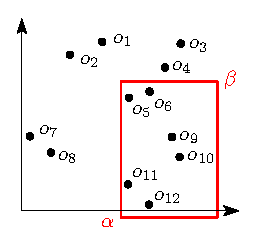
\includegraphics[width=.7\linewidth]{figs/aggregate-queries/example-object.eps}
    \caption{Objects}\label{fig:aggregate-queries:example:object}
  \end{subfigure}~%
  \begin{subfigure}[b]{.5\linewidth}
    \centering
    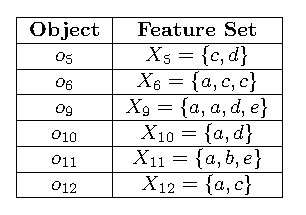
\includegraphics[width=.9\linewidth]{figs/aggregate-queries/example-feature.eps}
    \caption{Features}\label{fig:aggregate-queries:example:feature}
  \end{subfigure}
  \caption{Example of Aggregate Queries}\label{fig:aggregate-queries:example}
\end{figure}

\textbf{Aggregate Queries.} Since the results of aggregate queries are derived from aggregates of data, our study mainly focuses on the following primitive aggregate queries: \emph{max/min}, \emph{count}, \emph{sum}, \emph{top-$k$}, and \emph{frequent feature query (FFQ)}.\footnote{Extension to other more advanced aggregate queries such as \emph{average} and \emph{confidence} will be discussed in \Cref{sec:aggregate-queries:extension}.}  More specifically,  an aggregate query can be expressed in the form of $Q = (q, \{x_i\}, [\alpha, \beta])$, where $q$ is the aggregate operator, $\{x_i\}$ is the queried feature (which is only needed for \emph{count} and \emph{sum}), and $[\alpha, \beta]$ specifies the selection range on the non-sensitive attributes. Consider a sample query $Q = (q, \{x_i\}, [\alpha, \beta])$ in \Cref{fig:aggregate-queries:example}. The query range $[\alpha, \beta]$ selects the objects $o_5, o_6, o_9, o_{10}, o_{11}, o_{12}$. Since $X _5 \uplus X_6 \uplus X_9 \uplus X_{10} \uplus X_{11} \uplus X_{12} = \{(a, 6), (b, 1), (c, 4), (d, 3), (e, 2)\}$, the query result is based on the aggregate operator $q$, as follows:
\begin{itemize}
  \item $q=sum$ or $count$: This sums or counts the multiplicities of $\{x_i\}$ in all selected objects. Supposing $\{x_i\} = \{a\}$, the $sum$ and $count$ results are $(a, 6)$ and $(a, 4)$, respectively.\footnote{The $sum$ and $count$ results will be the same if there are no duplicate elements in the feature sets.}
  \item $q=max$ or $min$: This selects the feature with the maximum or minimum summed multiplicity in all selected objects. If $q=max$, the result is $(a, 6)$; if $q=min$, the result is $(b, 1)$. % chktex 35
  \item $q=$ \emph{top-$k$}: This selects the top-$k$ features with the largest summed multiplicities in all selected objects. Supposing $k$ = 3, the result is $(a, 6), (c, 4), (d, 3)$.
  \item $q=$ \emph{FFQ$_\delta$}: This selects the features whose summed multiplicities in all selected objects are no less than a threshold $\delta$. Supposing $\delta$ = 4, the result is $(a, 6), (c, 4)$.
\end{itemize}

The aggregate queries in \Cref{example:intro:pgp} can be reduced to the above aggregate queries as follows. \textbf{Q1} is simply a $max$ query, i.e., $(max, -, [95014, 95014])$. \textbf{Q2} is a \emph{count} query, i.e., $(count, \{\text{R-G1886S}\}, [00000, 99999])$. \textbf{Q3} is an FFQ query, $(FFQ_3, -, [20000, 29999])$, which finds the set of genes whose sum result is no less than 3. % chktex 35

\textbf{Threat Model and Problem Statement.} We consider two potential security threats:
\begin{inlineenum}
\item the SP could provide unfaithful query execution, thereby returning incorrect or incomplete query results; and
\item data privacy could be breached if sensitive source data are disclosed to the query client.
\end{inlineenum}
Thus, the authentication problem we are investigating is for the query client to verify that the SP executes $Q$ faithfully in terms of the following conditions:
\begin{inlineenum}
\item the candidate objects are correctly selected and no objects in the selection range are skipped;
\item the returned features and multiplicities are not tampered with; and
\item the query result satisfies the aggregation semantics.
\end{inlineenum}
The confidentiality requirement in this problem is to protect the objects' (sensitive) feature sets against the query client. That is, the client cannot infer the features (as well as their multiplicities) of any single object beyond what is implied from the query result.

If neither efficiency nor confidentiality is a concern, authenticating an aggregate query can work as follows. The SP returns a VO to the client, along with the query result. As a naive solution, the VO may include the non-sensitive attributes and sensitive features of all objects in $\mathbb{D}$ and a signature of $\mathbb{D}$. The client uses the VO to verify the soundness and completeness of the results by testing the following conditions:
\begin{itemize}
  \item None of the objects in $\mathbb{D}$ is tampered with.
  \item All candidate objects are in $[\alpha, \beta]$ and no objects in $[\alpha, \beta]$ are missing.
  \item The features and multiplicities of the candidate objects are correct.
  \item The result  satisfies the aggregation semantics of $q$.
\end{itemize}

However, the verification cost of this naive solution is prohibitively high because the entire dataset has to be returned. Moreover, verifying the last two conditions without disclosing sensitive feature sets requires privacy-preserving protocols. To address these issues, we propose an efficient privacy-preserving authentication framework based on verifiable multiset operations, the preliminaries of which are introduced in the next section.

\section{Preliminaries}\label{chap:aggregate-queries:prelim}

This section gives some preliminaries on cryptographic constructs and integrity assurance.

\textbf{Cryptographic Hash Function.}
A cryptographic hash function $H(\cdot)$ accepts an arbitrary-length string as its input and returns a fixed-length bit string. It is collision resistant, i.e., it is difficult to find two different messages $m_1$ and $m_2$ such that $H(m_1) = H(m_2)$. Classic cryptographic hash functions include SHA-1, SHA-2, and SHA-3.

\textbf{Bilinear-Map (BM) Accumulator.} This maps a multiset to a single value for ease of processing. Let $\mathbb{G}$ be a cyclic multiplicative group of order $p$. A BM accumulator is a function of a multiset $X$ of $n$ elements in the cyclic group $\mathbb{Z}_p$~\cite{10.1007/978-3-540-30574-3_19}. It returns an \emph{accumulative value} of $X$:
\begin{align}
  acc(X) = g^{P(X)} = g^{\prod_{x\in{X}}{(x+s)}},
\end{align}
where $g$ is a group generator of $\mathbb{G}$, $s \in \mathbb{Z}_p^* = \mathbb{Z}_p\backslash\{0\}$ is a random secret, and $P(X) = \prod_{x\in{X}}{(x+s)}$.

One useful property of $acc(X)$ is that even without knowing $s$, $acc(X)$ can still be computed by $X$ and $g, g^s, \dots, g^{s^k}$ ($k \ge |X|$) through polynomial interpolation. As for its security, it has been proved in~\cite{10.1007/s00453-014-9968-3} that the accumulative function $acc(\cdot)$ is collision resistant.

\textbf{Randomized BM Accumulator.} The above accumulative value $acc(X)$ is deterministic for a fixed multiset $X$. As such, an adversary can determine with high confidence that two multisets are the same if they happen to have the same accumulative value. To enhance confidentiality, we propose  randomizing the $acc$ value of $X$ as
\begin{align}
  acc(X) = g^{P(X) \cdot r_X},\label{eqn:aggregate-queries:random-bm}
\end{align}
where $r_X$ is a random value hidden from the query client but disclosed to the SP\@. It is worth noting that this randomization does not affect the original properties of a BM accumulator. We will further prove in \Cref{sec:aggregate-queries:security-analysis} that the randomized $acc$ values are indistinguishable under chosen plaintext attack.

\textbf{Bilinear Pairing.} This maps a pair of elements in two groups to a single element in a third group. Let $\mathbb{G}_{t}$ be another cyclic multiplicative group with the same order $p$. We can find a bilinear mapping $e: \mathbb{G} \times \mathbb{G} \rightarrow \mathbb{G}_t$ which has the following properties:
\begin{enumerate}
  \item \emph{Bilinearity}: If $u, v \in \mathbb{G}$ and $e(u,v)\in\mathbb{G}_t$, then $e(u^{a}, v^{b}) = e{(u, v)}^{ab}$ for any $u,v$.
  \item \emph{Non-degeneracy}: $e(g, g) \neq 1$.
  \item \emph{Computability}: Given $u,v\in \mathbb{G}$, it is easy to compute $e(u, v)$.
\end{enumerate}

\textbf{Bilinear $q$-Strong Diffie-Hellman (DH) Assumption.} This assumption shows that bilinear pairing is appropriate for multiset operation authentication as it is hard to forge. Let $(\mathbb{G}, \mathbb{G}_t, e, g)$ be a bilinear pairing. This assumption says that as long as $s\in \mathbb{Z}_p^*$ is secret, even given all elements $g, g^s, \dots, g^{s^k} \in \mathbb{G}$, no probabilistic polynomial-time (PPT) algorithm can derive ${e(g,g)}^{1/(x+s)}$ for any $x\in \mathbb{Z}_p^*$ with a probability higher than a negligible value~\cite{10.1007/978-3-540-28628-8_3}. In essence, this bilinear $q$-strong DH assumption extends the regular DH assumption on $g$ and $\mathbb{G}$ to $e(g,g)$ and $\mathbb{G}_t$. This assumption will be used as a foundation in our security analysis.

\textbf{Set Operation Authentication.} Based on the above, two result verification protocols have been introduced in~\cite{10.1007/978-3-642-54631-0_7,10.1007/978-3-642-22792-9_6} to authenticate the following operations on two sets $X_1$ and $X_2$:
\begin{inlineenum}
\item $X_1 \subseteq X_2$ and~\label{enum:aggregate-queries:prelim:set1}
\item $X_1 \cap X_2 = \emptyset$.~\label{enum:aggregate-queries:prelim:set2}
\end{inlineenum}

For~\ref{enum:aggregate-queries:prelim:set1}, the server computes a witness value $W = acc(X_2 - X_1)$ and returns it to the query client. The client then verifies $X_1 \subseteq X_2$ by checking:
\begin{align*}
  e(acc(X_1), W) \stackrel{?}{=} e(acc(X_2), g).
\end{align*}

For~\ref{enum:aggregate-queries:prelim:set2}, according to the extended Euclidean algorithm, there are two polynomials $Q_1, Q_2$ such that
\begin{align*}
  Q_1 \cdot P(X_1) + Q_2 \cdot P(X_2) = 1.
\end{align*}
As such, the server prepares $F_1 = g^{Q_1}, F_2 = g^{Q_2}$, and then the client verifies it by checking:
\begin{align*}
  e(F_1, acc(X_1)) \cdot e(F_2, acc(X_2)) \stackrel{?}{=} e(g,g).
\end{align*}
Though these two protocols are privacy-preserving in nature and can be extended to multisets, we have yet to design privacy-preserving authentication protocols for other multiset operations such as \emph{sum} and \emph{union}, which will be covered in \Cref{sec:aggregate-queries:multiset-op}.
%
\chapter{Authenticating Relational Queries with Fine-Grained Access Control}\label{chap:access-control}

In this chapter, we investigate the problem of authenticating relational queries with fine-grained access control. \Cref{sec:access-control:problem} introduces the formal problem definition, followed by cryptographic primitives in \Cref{sec:access-control:prelim}. \Cref{sec:access-control:equality-query} presents our solution for equality queries, which is then generalized to range queries and join queries in \Cref{sec:access-control:range-query} with the design of AP$^2$G-tree. A security analysis is presented in \Cref{sec:access-control:security-analysis}, and \Cref{sec:access-control:opt} and \Cref{sec:access-control:relaxing-zero-knowledge} present optimization techniques for the zero-knowledge model and a relaxed model, respectively. How to handle duplicate records and data updates are discussed in \Cref{sec:access-control:dup} and \Cref{sec:access-control:update} respectively. \Cref{sec:access-control:evluation} presents the experimental results, followed by a summary in \Cref{sec:access-control:summary}.

\section{Problem Formulation}\label{sec:access-control:problem}

\begin{figure}[t]
  \centering
  \resizebox{\linewidth}{!}{\begin{tikzpicture}[remember picture]
    \node (sp) {
        \begin{threeparttable}
            \begin{tabular}{|C|C|C|}
                \hline
                \multicolumn{3}{|c|}{\textbf{Database}} \\ \hline
                q\ attr. & content^{*} & \multicolumn{1}{c|}{access policy} \\ \hline
                o_1      & v_1              & Role_A \land Role_C           \\
                o_2      & v_2              & Role_A \land Role_B           \\
                o_3      & v_3              & Role_B \lor  Role_C           \\
                o_4      & v_4              & Role_C                        \\
                o_5      & v_5              & Role_A                        \\ \hline
            \end{tabular}
            \begin{tablenotes} \footnotesize
                \item[] \hspace{-0.2in} *Content is encrypted by CP-ABE
            \end{tablenotes}
        \end{threeparttable}
    };
    \node[below=0cm of sp] (sp-label) {\textbf{Service Provider (SP)}};

    \draw [red,rounded corners,thick]
    let \p1 = (sp.west),
    \p2 = ($(sp.south)!.26!(sp.north)$),
    \p3 = ($(sp.west)!.55!(sp.east)$),
    \p4 = ($(sp.south)!.59!(sp.north)$) in
    (\x1, \y2) rectangle (\x3, \y4)
    node[xshift=-0.32cm, yshift=-0.3cm] {$Q$};

    \node[matrix, left=-0.25cm of sp] {
        \node[scale=0.5] at (0,0) (do)
        {
\includegraphics{figs/icons/database.eps}};
        \draw[-latex] (0,0) -- (1.8,0)
        node [above,midway,font=\footnotesize]
        {$\{(o_i, v_i, \Upsilon_i)\}$}
        node [below,midway,font=\footnotesize]
        {$ADS$};
        \\
    };
    \node[xshift=0.5cm] at (sp-label -| do) {\textbf{Data Owner (DO)}};

    \node[matrix, right=-0.25cm of sp] (users) {
        \node[scale=0.9] at (0,0) (user1) {
\includegraphics{figs/icons/user.eps}};
        \node[below=0.1cm of user1,font=\footnotesize]{$Role_A, Role_B$};
        \node[right=0cm of user1]{$u_1$};

        \node[scale=0.9] at (0,-2) (user2) {
\includegraphics{figs/icons/user.eps}};
        \node[below=0.1cm of user2,font=\footnotesize]{$Role_C$};
        \node[right=0cm of user2]{$u_2$};

        \draw[-latex,transform canvas={yshift=0.5ex}] (0, 0) -- (-2.8, 0)
        node [above,midway,font=\small] {\textcolor{red}{$Q$}};
        \draw[-latex,transform canvas={yshift=-0.5ex}] (-2.8, 0) -- (0, 0)
        node [below,midway,font=\footnotesize,align=center] {$\{\langle o_2, v_2\rangle , \langle o_3, v_3\rangle\}$ \\ $VO$};

        \draw[-latex,transform canvas={yshift=0.5ex}] (0, -2) -- (-2.8, -2)
        node [above,midway,font=\footnotesize] {\textcolor{red}{$Q$}};
        \draw[-latex,transform canvas={yshift=-0.5ex}] (-2.8, -2) -- (0, -2)
        node [below,midway,font=\footnotesize,align=center] {$\{\langle o_3, v_3\rangle , \langle o_4, v_4\rangle\}$ \\ $VO$};
        \\
    };
    \node at (sp-label -| user1) (user-label) {\textbf{Clients}};
\end{tikzpicture}
}
  \caption{Query Authentication with Access Control}\label{fig:access-control:model}
\end{figure}

As shown in \Cref{fig:access-control:model}, there are three parties in the system:
\begin{inlineenum}
\item DO\@;
\item SP\@; and
\item clients.
\end{inlineenum}
The relational database $\mathcal{D}$, owned by the DO, is enforced with access control. Each record in $\mathcal{D}$ is a tuple $\langle o_i, v_i, \Upsilon_i\rangle$, where $o_i$ is the query attribute, $v_i$ is the content attribute, and $\Upsilon_i$ is the access policy. We assume that $o_i$ is discrete and distinct among all records.\footnote{The proposed approach is also applicable to continuous data which can be converted into discrete data by discretization techniques~\cite{Kotsiantis2006}. How to handle duplicate records will be discussed in \Cref{sec:access-control:dup}.} We further assume that $v_i$ is encrypted by CP-ABE~\cite{10.1109/sp.2007.11} (details in \Cref{sec:access-control:prelim}) for access control.\footnote{For simplicity, we assume that the query attribute is in plaintext. In cases where the query attribute is also encrypted,
privacy-preserving query techniques~\cite{10.1145/2699026.2699101} can be applied to retrieve query results, which is an orthogonal issue to query authentication.}
All the records are signed by the DO using an ADS and are outsourced to the SP, who answers queries from the clients on the behalf of the DO\@.

\textbf{System Setup.}
During the system setup, the DO generates a public key ${pk}_{client}$ (CP-ABE encryption key) and a secret key ${sk}_\text{DO}$ (ABS signing key), which can be used to encrypt the data and generate the ADS, respectively. The DO also distributes a secret key ${sk}_{client}$ (CP-ABE decryption key) and a public key ${pk}_\text{DO}$ (ABS verification key) to the clients, who can use them to decrypt and verify the query results, respectively.

\textbf{Access Policy.}
Access policies control the results of a query with respect to the roles of the client.\footnote{We use ``roles'' and ``attributes'' interchangeably in the context of ABE and ABS.}
For example, given the same range query $Q$ in \Cref{fig:access-control:model}, the result set to client $u_1$ with $Role_A$ and $Role_B$ is $\{\langle o_2, v_2\rangle$, $\langle o_3, v_3\rangle\}$ and that to client $u_2$ with $Role_C$ is $\{\langle o_3, v_3\rangle$, $\langle o_4, v_4\rangle\}$. In general, an access policy can be viewed as a boolean function in the form of $\Upsilon : {\{0, 1\}}^n \to \{0, 1\}$. It accepts multiple boolean inputs, each corresponding to a role, and outputs 1 or 0. For example, if $\Upsilon$ is defined as $({Role}_A \land {Role}_C) \lor {Role}_B$, then $\Upsilon({Role}_A) = 0$ and $\Upsilon({Role}_B, {Role}_C) = 1$. Here, for clarity, we omit those inputs with zero values (e.g., a singleton $Role_A$ implies that $Role_B$ and $Role_C$ are missing). While, technically, an access policy can take any boolean function, in the literature, most works focus on a specific type, namely, monotone boolean functions~\cite{10.1145/1180405.1180418,10.1109/sp.2007.11,10.1007/978-3-642-19074-2_24,10.1145/1755688.1755697}. Formally, the monotonic property means that, for all $a_i$ and $b_i$ in $\{0, 1\}$, if $a_1 \le b_1$, $\dots$, $a_n \le b_n$, then $\Upsilon(a_1, \dots, a_n) \le \Upsilon(b_1, \dots, b_n)$ holds. This property suggests that a client with more roles has a higher clearance level and so can access more data. % chktex 8
For simplicity, we assume that all access control policies are monotone boolean functions that are normalized in a \emph{disjunctive normal form} (DNF).

\textbf{Threat Model.}
Two security threats are considered in our problem:
\begin{inlineenum}
\item the SP is not fully trusted and it might return tampered or incomplete query results; and
\item the clients are curious and may want to learn the information about the data to which access is unauthorized.
\end{inlineenum}

To address the first threat, we advocate authenticated query processing. Specifically, during query processing, the SP traverses the ADS and constructs a VO that includes the verification information of the results. The VO is returned to the client along with the results. Using the VO, the client should establish the \emph{soundness} and \emph{completeness} of a result set $RS$:
\begin{itemize}
  \item \textbf{Soundness}. No records in $RS$ are tampered with and are truly the results with respect to the roles of the client.
  \item \textbf{Completeness}. All records not in $RS$ are either non-results or are inaccessible to the client.
\end{itemize}
Take the range query $Q$ in \Cref{fig:access-control:model} as an example. $RS=\{\langle o_2, v_2\rangle$, $\langle o_3, v_3\rangle\}$ is the correct result set for client $u_1$. $RS_1 = \{\langle o_2, v_2'\rangle$, $\langle o_3, v_3\rangle\}$ and $RS_2 = \{\langle o_2, v_2\rangle$, $\langle o_3, v_3\rangle$, $\langle o_4, v_4\rangle\}$ are not sound because they either contain fake ($v_2'$ in $RS_1$) or inaccessible ($o_4$ in $RS_2$) records. $RS_3 = \{\langle o_2, v_2\rangle\}$ is not complete because $o_3$ is missing.

To further address the second threat, we need to protect data access against unauthorized clients during query authentication. We define three levels of confidentiality requirements:
\begin{itemize}
  \item \textbf{Data Content Confidentiality}. The contents of inaccessible records are protected. This is a basic requirement for any query service that supports access control.
  \item \textbf{Access Policy Confidentiality}. In addition to data content confidentiality, the access policies of inaccessible records are protected. That is, the clients must not know that their denied access is due to the lack of some specific role(s). % chktex 36
  \item \textbf{Zero-Knowledge Confidentiality}.
    Any information beyond the accessible records $\mathcal{D}^+$ in the database $\mathcal{D}$ is protected. That is, the clients can gain nothing about $\mathcal{D}\backslash\mathcal{D}^+$ (e.g., not even its size or the associated access policies).
\end{itemize}
The above security notions will be formalized when we perform security analysis in \Cref{sec:access-control:security-analysis-query}. We assume that there is no collusion between the SP and clients.

In what follows, we propose a zero-knowledge query authentication solution that addresses both of the security threats under fine-grained access control. We will develop new query authentication techniques for ADS generation, VO construction, and result verification that achieve the zero-knowledge confidentiality. To cater for performance-centric applications, we will also discuss how to further improve the query authentication performance by relaxing the confidentiality requirement.

\section{Preliminaries}\label{sec:access-control:prelim}

This section gives some preliminaries on cryptographic constructs and integrity assurance.

\textbf{Cryptographic Hash Function.}
A cryptographic hash function $H(\cdot)$ accepts an arbitrary-length string as its input and returns a fixed-length bit string. It is collision resistant; it is difficult to find two different messages, $m_1$ and $m_2$, such that $H(m_1) = H(m_2)$. Classic cryptographic hash functions include the SHA-1, SHA-2, and SHA-3 family.

\textbf{Bilinear Pairing.}
Bilinear pairing maps a pair of elements in two groups to a single element in a third group, which serves as a basic operation in \emph{attribute-based encryption} (ABE) and \emph{attribute-based signature} (ABS), as shown later in this chapter.

Let $\mathbb{G}$, $\mathbb{H}$, and $\mathbb{G}_T$ be three cyclic multiplicative groups with the same order $p$, where $p$ is a prime. Let $g$, $h$ be the generator of $\mathbb{G}$ and $\mathbb{H}$, respectively. We can find a bilinear mapping $e: \mathbb{G} \times \mathbb{H} \rightarrow \mathbb{G}_T$, which has the following properties:
\begin{itemize}
  \item \textsf{Bilinearity}: If $u \in \mathbb{G}$, $v \in \mathbb{H}$, and $e(u,v)\in\mathbb{G}_T$, then $e(u^a, v^b) = {e(u, v)}^{ab}$ for any $u,v$.
  \item \textsf{Non-degeneracy}: $e(g, h) \neq 1$.
\end{itemize}

\textbf{Ciphertext-Policy Attribute-Based Encryption (CP-ABE).}
CP-ABE is proposed to realize complex access control over encrypted data~\cite{10.1109/sp.2007.11}. By embedding the access policy into the ciphertext, it enables fine-grained access control represented by a boolean function of attributes.
It consists of a set of algorithms:
\begin{itemize}
  \item \textsf{CP-ABE.Setup}$(1^\lambda) \to (mk, pp)$:
    On input a security parameter $1^\lambda$, it generates a master private key $mk$ and a public key $pp$.
  \item \textsf{CP-ABE.KeyGen}$(mk, \mathcal{A}) \to {sk}_\mathcal{A}$:
    On input a master private key $mk$ and an attribute set $\mathcal{A}$, it outputs a decryption key ${sk}_\mathcal{A}$.
  \item \textsf{CP-ABE.Encrypt}$(pp, x, \Upsilon) \to c_{\Upsilon}$:
    On input a public key $pp$ and an access policy $\Upsilon$, it encrypts plaintext $x$ into ciphertext $c_\Upsilon$.
  \item \textsf{CP-ABE.Decrypt}$({sk}_\mathcal{A}, c_\Upsilon) \to x$:
    On input a decryption key ${sk}_\mathcal{A}$, ciphertext $c_\Upsilon$, it outputs plaintext $x$ if $\Upsilon(\mathcal{A}) = 1$; otherwise $\bot$ is returned.
\end{itemize}

\textbf{Attribute-Based Signature (ABS).}
Introduced in~\cite{10.1007/978-3-642-19074-2_24}, ABS is a signature scheme that enables a party to sign a message with fine-grained access control over the identifying information. Unlike a traditional signature scheme, messages can be signed with a monotone boolean function predicate that is satisfied by the attributes obtained from the authority. It consists of the following algorithms:
\begin{itemize}
  \item \textsf{ABS.Setup}$(1^\lambda) \to (msk, mvk)$:
    On input a security parameter $1^\lambda$, it generates a master signing key $msk$ and a master verification key $mvk$.
  \item \textsf{ABS.KeyGen}$(msk, \mathcal{A}) \to {sk}_\mathcal{A}$:
    On input a master signing key $msk$ and an attribute set $\mathcal{A}$, it outputs a signing key ${sk}_\mathcal{A}$.
  \item \textsf{ABS.Sign}$({sk}_\mathcal{A}, m, \Upsilon) \to \sigma_{m,\Upsilon}$:
    On input a signing key ${sk}_\mathcal{A}$, a message $m$, and a monotone boolean function predicate $\Upsilon$, where $\Upsilon(\mathcal{A}) = 1$, it outputs a signature $\sigma_{m,\Upsilon}$.
  \item \textsf{ABS.Verify}$(mvk, m, \Upsilon, \sigma_{m,\Upsilon}) \to \{0, 1\}$:
    On input a master verification key $mvk$, an unverified message $m$, an unverified monotone boolean function predicate $\Upsilon$, and a signature $\sigma_{m,\Upsilon}$, it outputs 1 if the signature is valid.
\end{itemize}

More elaborate procedures, along with extended algorithms, will be given in \Cref{sec:access-control:abs}.

\section{Equality Query Authentication}\label{sec:access-control:equality-query}

A naive solution to query authentication with fine-grained access control is to use the Merkle hash tree~\cite{10.1007/0-387-34805-0_21} to construct a VO for authenticated query processing and to use CP-ABE to encrypt data records for access control. More specifically, for any query, all data records (including those inaccessible ones) that lie in the query range, along with the VO, are returned to the client. After verifying the records, the client can decrypt and access the authorized records, using the attribute secret key obtained from the DO\@. However, this solution has two problems. First, it will return a large number of inaccessible records to the client, which incurs high computation and communication overheads. Second, for the inaccessible records, thanks to CP-ABE, although they cannot be decrypted by the client, returning them still reveals some information about their existence and their access policies. This violates our zero-knowledge confidentiality requirement.

In the following, we propose new query authentication techniques that support both fine-grained access control and zero-knowledge confidentiality. We start with equality queries by developing a novel signature scheme in this section and then extend it to range queries and join queries in \Cref{sec:access-control:range-query}.

In an equality query, the client specifies a query key $o_q$ as well as his/her access role set $\mathcal{A}$. Since the query attribute is distinct, there could be three possible outcomes:
\begin{itemize}
  \item There is one record matching $o_q$ and it is accessible to the query client.
  \item There is one record matching $o_q$ but it is not accessible to the query client.
  \item There is no record matching $o_q$.
\end{itemize}

Recalling our zero-knowledge confidentiality does not allow the client to distinguish between the last two outcomes. To prevent the information leakage caused by non-existent records, we introduce a global pseudo access role, ${Role}_{\emptyset}$, which is not possessed by any client. We treat each non-existent record as a \emph{pseudo} record that is associated with the access policy ${Role}_{\emptyset}$. As such, for any equality query, there is always one matching record with one of the two possible outcomes: accessible or inaccessible.

\subsection{ADS Generation and Query Processing}

\textbf{ADS Generation.} Our construction for zero-knowledge query authentication is built upon a novel signature scheme. During the system setup, the DO generates a signature for each data record. These signatures, serving as ADS, are sent to the SP, who will then use them to support verifiable queries. As mentioned earlier, the signature has two design requirements. First, given a record $i$, the signature should capture all of its three components (query attribute $o_i$, data content $v_i$, and access policy $\Upsilon_i$) so that it can be used as a proof of integrity. Second, in case the record is inaccessible to some clients, the signature can be tailored to prove the inaccessibility with the zero-knowledge confidentiality. To this end, we propose a new access-policy-preserving (APP) signature based on a variant of the ABS (to be detailed in \Cref{sec:access-control:abs}).

\begin{definition}[APP Signature] Consider a record $\langle o_i$, $v_i$, $\Upsilon_i\rangle$. Let ${sk}_{\textrm{DO}}$ be the signing key of the DO, $H(\cdot)$ a cryptographic hash function, and `$|$' denote string concatenation. The access-policy-preserving (APP) signature for this record is generated as:
  \begin{align*}
    \sigma_i & = \textsf{ABS.Sign}({sk}_{\textrm{DO}}, H(o_i) | H(v_i) , \Upsilon_i)
  \end{align*}
  In the case of pseudo (non-existent) records, $v_i$ will be assigned a random value and $\Upsilon_i$ will be ${Role}_{\emptyset}$.
\end{definition}

\begin{figure}[t]
  \centering
  \resizebox{\linewidth}{!}{\begin{tikzpicture}
    \node[matrix] (users) {
        \node[scale=0.9] at (0,0) (user1) {
\includegraphics{figs/icons/user.eps}};
        \node[below=0cm of user1]{$Role_A, Role_B$};
        \node[right=0cm of user1]{$u_1$};

        \node[scale=0.9] at (0,-2) (user2) {
\includegraphics{figs/icons/user.eps}};
        \node[below=-0.1cm of user2]{$Role_C$};
        \node[right=-0.1cm of user2]{$u_2$};
        \\
    };

    \coordinate (user_mid) at ($(user1)!.5!(user2)$);

    \node (aps) [left=3.5cm of user2,align=center] {APS signature\\$\hat{\sigma}_{2, \mathcal{A}_{u_2}}$};
    \node [draw,thick,fit=(aps),rounded corners] (aps_round) {};

    \node (app) [left=6cm of user1,align=center] {APP signature\\$\sigma_2$};
    \node [draw,thick,fit=(app),rounded corners] (app_round) {};

    \node (data) [left=10cm of user2,align=center]
    {$\langle o_2, v_2, \Upsilon_2\rangle$\\$\Upsilon_2 = Role_A \land Role_B$};
    \node [draw,thick,fit=(data),rounded corners] (data_round) {};

    \draw[-latex, thick] (app_round.east) -- ($(user1) - (0.5cm, 0)$)
    node [above,midway] (vo1) {};
    \draw[-latex, thick] (aps_round.east) -- ($(user2) - (0.5cm, 0)$)
    node [above,midway] (vo2) {$\langle H(v_2), \hat{\sigma}_{2, \mathcal{A}_{u_2}}\rangle$};
    \draw (vo2 |- vo1) node [above] {$\langle v_2, \sigma_2, \Upsilon_2\rangle$};

    \draw[-latex, thick] (app_round.south) .. controls (app_round.south |- aps_round.west)
                          .. (aps_round.west)
    node[below,midway,pos=0.55,xshift=-0.2cm,yshift=-0.1cm] {\textsf{ABS.Relax}};

    \draw[-latex, thick] (data_round.north) .. controls (data_round.north |- app_round.west)
                          .. (app_round.west)
    node[above,midway,pos=0.75] {\textsf{ABS.Sign}};

    \coordinate (do_sp_mid) at ($(data_round.east)!.5!(app_round.west)$);
    \draw[dashed, color=black!30] ($(do_sp_mid) - (0,1.8cm)$) -- ($(do_sp_mid) + (0,1.5cm)$);

    \coordinate (sp_user_mid_x) at ($(aps_round.east) + (0.2cm, 0)$);
    \coordinate (sp_user_mid) at (do_sp_mid -| sp_user_mid_x);
    \draw[dashed, color=black!30] ($(sp_user_mid) - (0,1.8cm)$) -- ($(sp_user_mid) + (0,1.5cm)$);

    \node[below=0.15cm of data_round.south] (do-label) {\textbf{Data Owner (DO)}};
    \draw let \p1 = ($(sp_user_mid)!0.5!(do_sp_mid)$), \p2 = (do-label) in (\x1, \y2)
    node {\textbf{Service Provider (SP)}};
    \node at (do-label -| user1) (user-label) {\textbf{Clients}};
\end{tikzpicture}
}
  \caption{Equality Query Authentication}\label{fig:access-control:equality-query}
\end{figure}

\textbf{Authenticated Query Processing.}
After the SP receives the APP signatures for all records from the DO, it is able to support authenticated query processing by constructing a VO for the query result.
\Cref{fig:access-control:equality-query} shows an example of two different clients issuing an equality query with key $o_2$.
Client $u_1$ is allowed to access the record $o_2$, so it is straightforward to return the APP signature generated by the DO as the VO\@. That is, the SP will return $\langle v_2$, $\sigma_2 = \textsf{ABS.Sign}({sk}_\text{DO}$, $H(o_2) | H(v_2)$, $\Upsilon_2)$, $\Upsilon_2\rangle$. On the client side, $H(o_2) | H(v_2)$ will be computed based on the query attribute $o_2$ and the result $v_2$ returned by the SP\@. If it can be verified by the signature $\sigma_2$ under the policy $\Upsilon_2$, $\langle o_2, v_2\rangle$ is a genuine result. % chktex 36

Next, we consider the case in which the data record is inaccessible to the client (e.g., $u_2$ in \Cref{fig:access-control:equality-query}). Since the query attribute is distinct, we only need to prove the inaccessibility of this data record. Simply returning the APP signature does not work, because this would disclose the access policy and hence the specific reason why the client cannot access the record. To achieve the zero-knowledge confidentiality, the SP can only leverage the information which is already known to the client to prove the inaccessibility. Specifically, the global access role set $\mathbb{A}$ and the client's own role set $\mathcal{A}$ are such information the SP can use.

In a monotone boolean function, given an access role set as input, the reason for it to output 0 is only because it lacks one or more roles in $\mathbb{A}\backslash\mathcal{A}$ (i.e., those roles that the client does not own). Thus, our idea is to make use of a \emph{super} access policy, denoted by $\hat{\Upsilon}_{\mathcal{A}}$, that does not honor the role set $\mathcal{A}$. More specifically, it is a boolean function that fuses each role in $\mathbb{A}\backslash\mathcal{A}$ using the OR operator. For example, in \Cref{fig:access-control:equality-query}, if the access role universe $\mathbb{A}$ is $\{{Role}_{\emptyset}$, ${Role}_A$, ${Role}_B$, ${Role}_C\}$,
then
$\hat{\Upsilon}_{\{{Role}_C \}}$ = ${Role}_{\emptyset} \lor {Role}_A \lor {Role}_B$ for client $u_2$. In essence, it is the weakest access policy under which the client still cannot access the record. Based on this concept, we define the following access-policy-stripped (APS) signature that embeds the super access policy.

\begin{definition}[APS Signature]
  Consider a record $\langle o_i$, $v_i$, $\Upsilon_i\rangle$. Denoted by $\mathbb{A}$ and $\mathcal{A}$ the global access role set and the query client's role set, respectively. Let ${sk}_{\textrm{DO}}$ be the signing key of the DO, $H(\cdot)$ a cryptographic hash function, and `$|$' denote string concatenation. The access-policy-stripped (APS) signature for this record and the client with access role set $\mathcal{A}$ is defined as:
  \begin{align*}
    \hat{\sigma}_{i, \mathcal{A}} & = \textsf{ABS.Sign}({sk}_{\textrm{DO}}, H(o_i) | H(v_i) , \hat{\Upsilon}_{\mathcal{A}}),
  \end{align*}
  where $\hat{\Upsilon}_{\mathcal{A}} = a_1 \lor a_2 \lor \dots \lor a_n, \quad a_i \in \mathbb{A}\backslash\mathcal{A}$.
\end{definition}

\begin{algorithm}[t]
  \caption{Authentication of Equality Queries}\label{alg:access-control:equality-query}
  \SetKwBlock{DO}{ADS Generation (by the DO)}{}
  \SetKwBlock{SP}{VO Construction (by the SP)}{}
  \SetKwBlock{Client}{Result Verification (by the client)}{}
  \SetKw{forin}{in}
  \DO{%
    \For{each data record $\langle o_i, v_i, \Upsilon_i\rangle$}{%
      $\sigma_i \gets \textsf{ABS.Sign}({sk}_{\textrm{DO}}, H(o_i) | H(v_i) , \Upsilon_i)$\;
    }
    Outsource all records $\langle o_i, v_i, \Upsilon_i, \sigma_i\rangle$ to the SP\;
  }
  \SP{%
    \KwIn{Query attribute $o_q$, access role set $\mathcal{A}$}
    \lIf{$\Upsilon_{o_q}(\mathcal{A}) = 1$}{%
      $VO \gets \langle v_{o_q}, \sigma_{o_q}, \Upsilon_{o_q}\rangle$%
    }
    \Else{%
      $\hat{\sigma}_{o_q,\mathcal{A}} \gets \textsf{ABS.Relax}(\sigma_{o_q}, \mathbb{A}\backslash\mathcal{A})$
      \tcp*{\Cref{sec:access-control:abs}}
      $VO \gets \langle H(v_{o_q}), \hat{\sigma}_{o_q,\mathcal{A}}\rangle$\;
    }
    send $\textsf{CP-ABE.Encrypt}(pp, VO, \land_{a \in \mathcal{A}} a)$ to the client\;
  }
  \Client{%
    run \textsf{CP-ABE.Decrypt} to decrypt the VO\;
    \eIf{$\Upsilon_{o_q}(\mathcal{A}) = 1$}{%
      run \textsf{ABS.Verify}$(mvk, H(o_q)|H(v_{o_q}), \Upsilon_{o_q}, \sigma_{o_q})$\;
      }{%
      $\hat{\Upsilon}_{\mathcal{A}} \gets \lor_{a \in \mathbb{A}\backslash\mathcal{A}} a$\;
      run \textsf{ABS.Verify}$(mvk, H(o_q)|H(v_{o_q}), \hat{\Upsilon}_{\mathcal{A}}, \hat{\sigma}_{o_q,\mathcal{A}})$\;
    }
  }
\end{algorithm}

The APS signature, which can be derived from the APP signature (see \Cref{sec:access-control:abs} for details), serves as the VO for an inaccessible record. % chktex 36
By the embedded super access policy, the client is able to verify the inaccessibility, but cannot infer the specific roles he/she lacks.
In the running example of \Cref{fig:access-control:equality-query}, for client $u_2$, the SP will return $\langle H(v_2)$, $\hat{\sigma}_{2, \mathcal{A}_{u_2}} = \textsf{ABS.Sign}({sk}_\text{DO}$, $H(o_2) | H(v_2)$, $\hat{\Upsilon}_{\{{Role}_C \}})\rangle$. During result verification, $H(o_2) | H(v_2)$ will be computed by the client based on the query attribute $o_2$ and the value $H(v_2)$ returned by the SP, and $\hat{\Upsilon}_{\{{Role}_C \}}$ will be computed from the client's access role set. With these components, the client can verify the super policy $\hat{\Upsilon}_{\{{Role}_C \}}$ via the APS signature $\hat{\sigma}_{2, \mathcal{A}_{u_2}}$ to prove that the record is indeed inaccessible to the client. % chktex 1 chktex 36

Finally, to prevent impersonation attacks, the SP will encrypt the query result as well as the VO using a traditional one-key cipher, such as AES, with the one-key cipher key encrypted using CP-ABE under the access policy $a_1 \land a_2 \land \dots \land a_n$, $a_i \in \mathcal{A}$. Therefore, only the query client who indeed has the access role set $\mathcal{A}$ as claimed can decrypt the query result.

\Cref{alg:access-control:equality-query} summarizes the procedures discussed above for authenticating equality queries with the zero-knowledge confidentiality.
\subsection{ABS with Predicate Relaxation}\label{sec:access-control:abs}

In this section, we develop a variant of the ABS scheme, which supports predicate relaxation on super access policies and hence can be used to generate the APP signature\@.

\subsubsection{Monotone Span Program}\label{sec:access-control:msp}

To build the ABS scheme, we first introduce the monotone span program, which is a special form of matrix that can be used to present its equivalent monotone boolean function. It is defined as follows.

\begin{definition}[Monotone Span Program]
  Let $\Upsilon : {\{0, 1\}}^n \to \{0, 1\}$ be a monotone boolean function. A monotone span program for $\Upsilon$ over a field $\mathbb{F}$ is an $\ell \times t$ matrix $\mathbf{M}$ with entries $\mathbb{F}$, with a labeling function $a: [\ell] \to [n]$, which associates each row of $\mathbf{M}$ with an input variable of $\Upsilon$. For every $(x_1, \dots, x_n) \in {\{0, 1\}}^n$, it satisfies the following:
  \begin{align*}
    \Upsilon(x_1, \dots, x_n) = 1 \Longleftrightarrow & \ \exists \mathbf{v} \in \mathbb{F}^{1 \times \ell}: \mathbf{v}\mathbf{M} = [1, 0, 0, \dots, 0] \\
                                                      & \text{ and } (\forall i: x_{a(i)} = 0 \Rightarrow \mathbf{v}_i = 0)
  \end{align*}
\end{definition}

In other words, $\Upsilon(x_1, \dots, x_n) = 1$ if and only if the rows of $\mathbf{M}$ indexed by $\{i~|~x_{a(i)} = 1 \}$ span the vector $[1, 0, 0, \dots, 0]$.

There are many different approaches to constructing a monotone span program from a monotone boolean function~\cite{Nikov:2004,Liu:2010}.
In our construction, we choose a recursive algorithm as shown in \Cref{alg:access-control:msp}, which accepts a boolean function expressed in AND and OR operators as inputs~\cite{Nikov:2004}.

\begin{algorithm}[t]
  \caption{Build Monotone Span Program}\label{alg:access-control:msp}
  \SetKwFunction{BuildMSP}{BuildMSP}
  \SetKw{is}{is}
  \SetKw{forin}{in}
  \Fn{\BuildMSP{expr}}{%
    \KwIn{Boolean Function $expr$}
    \KwOut{Span Program $\mathbf{M}$, Row Labels $L$}
    \eIf{$expr$ \is~label}{%
      $\mathbf{M} \gets (1)$,
      $L \gets [expr]$\;
      }{%
      $n \gets \textrm{len}(expr.children)$\;
      \Switch{$expr$ type}{%
        \uCase{AND operator}{%
          $\mathbf{M} \gets \underset{n \times n}{\begin{pmatrix}
              1 & -1 & \cdots & -1 \\
              0 & 1  & \cdots & 0 \\
              \vdots & \vdots & \ddots & \vdots \\
              0 & 0 & \cdots & 1
          \end{pmatrix}}
          $\;
        }
        \Case{OR operator}{%
          $\mathbf{M} \gets \underset{n \times 1}{{(1, \dots, 1)}^T}$\;
        }
      }
      $i \gets 1, L \gets []$\;
      \For{$e$ \forin~$expr.children$}{%
        $\mathbf{M}_e, L_e \gets \BuildMSP{e}$\;
        $\mathbf{M} \gets \begin{pmatrix}
          \mathbf{M}[1\!:\!i-1, :] & 0 \\
          \mathbf{M}_e[:, 1] \cdot \mathbf{M}[i, :] & \mathbf{M}_e[:, 2\!:] \\
          \mathbf{M}[i+1\!:, :] & 0
        \end{pmatrix}
        $\;
        $L \gets L + L_e$, $i \gets i + \textrm{\# of rows}(\mathbf{M}_e)$\;
      }
    }
    \Return{$\langle \mathbf{M}, L\rangle$}\;
  }
\end{algorithm}

\subsubsection{ABS Construction}\label{sec:access-control:abs-cons}
\newcommand{\hash}{\textsf{hash}}

Derived from the Practical Instantiation 4 in~\cite{10.1007/978-3-642-19074-2_24}, our ABS construction consists of the following algorithms.

\textsf{ABS.Setup}$(1^\lambda) \to (msk, mvk)$:
Let $(\mathbb{G}$, $\mathbb{H}$, $\mathbb{G}_T$, $e)$ be a bilinear pairing.
Choose random generators:
\begin{align*}
  g, C \gets \mathbb{G}; & \qquad h_0, h \gets \mathbb{H}.
  \intertext{Choose random values $a_0,a,b \gets \mathbb{Z}_p$ and compute:}
  A_0 = h_0^{a_0};       & \qquad A = h^a\textrm{ and } B = h^b.
\end{align*}

The master signing key is $msk = (a_0, a, b)$, and the master verifying key is $mvk = (g, h_0, h, A_0, A, B, C)$.

\textsf{ABS.KeyGen}$(msk, \mathcal{A}) \to {sk}_\mathcal{A}$:
Choose random value $K_{\mathrm{base}} \gets \mathbb{G}$. The signing key is computed as:
\begin{align*}
  {sk}_\mathcal{A} = (
  K_{\mathrm{base}},K_0 = K_{\mathrm{base}}^{1/a_0},
  \{ K_u = K_{\mathrm{base}}^{1/(a+bu)}| u \in \mathcal{A}\}
  ).
\end{align*}

\textsf{ABS.Sign}$({sk}_\mathcal{A}, m, \Upsilon) \to \sigma_{m, \Upsilon}$:
Convert $\Upsilon$ to its corresponding monotone span program $\mathbf{M} \in \mathbb{Z}_p^{\ell \times t}$, with row labeling $u: [\ell] \to \mathbb{A}$, where $\mathbb{A}$ denotes the universe of attributes. Also compute the vector $\mathbf{v} = [v_0, \dots, v_\ell]$ that corresponds to the satisfying attributes $\mathcal{A}$. Pick random values $\tau, r_0, r_1, \dots, r_\ell \gets \mathbb{Z}_p$. The signature is composed as:
\begin{align*}
    & \sigma_{m,\Upsilon} = (\tau,Y,W,S_1,\dots,S_\ell,P_1,\dots,P_t);    \\
    &\begin{array}{l@{}ll@{}ll}
      Y & = K_{\mathrm{base}}^{r_0}; &
      S_i& = K_{u(i)}^{v_i \cdot r_0} \cdot {(C g^{\hash})}^{r_{i}}
         & (\forall i \in [\ell]);
         \\
      W & = K_0^{r_0};               &
      P_j& = \prod_{i=1}^\ell{(A B^{u(i)})}^{\mathbf{M}_{ij}\cdot r_{i}}
         & (\forall j \in [t]).
    \end{array}
\end{align*}
Here $\hash = H(\tau, m)$ for some collision-resistant hash function $H(\cdot)$.
%
Note that the signer may not have $K_{u(i)}$ for every attribute mentioned in the claim-predicate. However, in such cases, $v_i=0$.

\textsf{ABS.Verify}$(mvk, m, \Upsilon, \sigma_{m, \Upsilon}) \to \{0,1\}$:
To verify the signature, the verifier converts $\Upsilon$ to its corresponding monotone span program $\mathbf{M} \in \mathbb{Z}_p^{\ell \times t}$, with row labeling $u: [\ell] \to \mathbb{A}$. The signature is valid if and only if all of the following constraints hold:
\begin{align*}
  Y         \stackrel{?}{\neq} 1; \quad & \quad e(W,A_0)  \stackrel{?}{=} e(Y,h_0); \\
  \prod_{i=1}^\ell e \left( S_i, {(A B^{u(i)})}^{\mathbf{M}_{ij}}\right)
                                        & \stackrel{?}{=}  \left\{
                                          \begin{array}{ll}
                                            e(Y,h)e(Cg^{\hash},P_1)             & \text{if } j = 1,                        \\
                                            e(Cg^{\hash},P_j)                   & \text{if } j > 1.
                                        \end{array} \right.
\end{align*}

\subsubsection{Predicate Relaxation}\label{sec:access-control:abs-relax}

Our ABS scheme supports predicate relaxation. This enables the SP to derive new signatures on super access policies. It works as follows.

\textsf{ABS.Relax}$(\sigma_{m,\Upsilon}, \mathcal{A}') \to \sigma_{m,\Upsilon'}$:
Given a signature $\sigma_{m,\Upsilon}$ signed under predicate $\Upsilon$ and an attribute set $\mathcal{A}'$, this operation outputs a new signature $\sigma_{m,\Upsilon'}$ signed under the new predicate $\Upsilon' = \lor_{a \in \mathcal{A}'} a$. It can succeed if and only if $\Upsilon'(\mathcal{A}) = 1$, $\forall \mathcal{A} \in \{ A~|~\Upsilon(A) = 1, A \subseteq \mathbb{A} \}$. In other words, $\mathcal{A}'$ should satisfy the condition $\Upsilon(\mathbb{A}\backslash\mathcal{A}') = 0$.
For example, in \Cref{fig:access-control:model}, the APP signature of $o_2$ has the predicate $\Upsilon_2 = {Role}_{A} \land {Role}_{B}$. By invoking \textsf{ABS.Relax}, it can be relaxed to a new signature, the predicate of which is $\Upsilon_2' = {Role}_{\emptyset} \lor {Role}_{A} \lor {Role}_{B}$, for client $u_2$ (i.e., $u_2$'s super access policy), because $\Upsilon_2(\mathbb{A}\backslash \{{Role}_{\emptyset}, {Role}_A, {Role}_B\}) = \Upsilon_2(\{{Role}_C\}) = 0$. However, relaxing it to a signature, say with predicate $\Upsilon_2'' = {Role}_{\emptyset} \lor {Role}_{C}$, will fail, as $\Upsilon_2(\mathbb{A}\backslash \{{Role}_{\emptyset}, {Role}_C\}) = \Upsilon_2(\{{Role}_A, {Role}_B\}) = 1$.

The overall procedure is summarized in \Cref{alg:access-control:abs-relax}. It consists of the following steps:
\begin{algorithm}[t]
  \caption{\textsf{ABS.Relax}}\label{alg:access-control:abs-relax}
  \SetKwFunction{ABSRelax}{ABS.Relax}
  \SetKwFunction{Purge}{Purge}
  \SetKw{is}{is}
  \SetKw{forin}{in}
  \SetKw{forto}{to}
  \Fn{\ABSRelax{$\sigma_{m, \Upsilon}, \mathcal{A}'$}}{%
    \KwIn{ABS signature $\sigma_{m, \Upsilon}$, attribute set $\mathcal{A}'$}
    \KwOut{ABS signature $\sigma_{m, \Upsilon'}$, where $\Upsilon' = \lor_{a\in\mathcal{A}'} a$}
    $\langle \tau, Y, W, \{S_i\}, \{P_j\}\rangle \gets \sigma_{m, \Upsilon}$\;
    \tcp{step 1: purging unwanted attributes}
    $\langle rows, cols, L, kept\_rows, kept\_cols, flag\rangle\gets$\Purge{$\Upsilon, \mathcal{A}'$}\;
    \lIf{$flag$~\is~false}{\textbf{abort}}
    $\tilde{P}_1 \gets \prod_{j \in kept\_cols} P_j$\;
    \For{$i = 1~\forto~\text{len}(\mathcal{A}')$}{%
      $u \gets \mathcal{A}'[i]$\;
      \eIf{$u \in \{L[l] | l \in kept\_rows\}$}{%
        \tcp{step 2: merging duplicate attributes}
        $\tilde{S}_i \gets \prod_{k \in \{l| L[l] = u\}} S_k$\;
        }{%
        \tcp{step 3: appending missing attributes}
        $r \gets \text{random value}$,
        $\tilde{S}_i \gets {(Cg^{\hash})}^r$,
        $\tilde{P}_1 \gets \tilde{P}_1 \cdot {(AB^{u})}^r$\;
      }
    }
    \tcp{step 4: re-randomizing signature}
    $r \gets \text{random value}$,
    $\sigma_{m, \Upsilon'} \gets \langle \tau, Y^r, W^r, \{\tilde{S}_i^r\}, \tilde{P}_1^r\rangle$\;
    \Return{$\sigma_{m, \Upsilon'}$}\;
  }
\end{algorithm}

\begin{algorithm}[thp]
  \caption{\textsf{ABS.Relax} Purging Step}\label{alg:access-control:abs-relax-purge}
  \SetKwFunction{Purge}{Purge}
  \SetKw{is}{is}
  \SetKw{forin}{in}
  \SetKw{forto}{to}
  \Fn{\Purge{$expr$, $\mathcal{A}$}}{%
    \KwIn{Boolean Function $expr$, kept attribute set $\mathcal{A}$}
    \KwOut{Monotone Span Program size $\langle rows, cols\rangle$, Row Labels $L$,
      Rows and Columns in MSP to be kept $\langle kept\_rows$, $kept\_cols\rangle$,
      Whether to keep this node $flag$
    }
    \eIf{$expr$ \is~label}{%
      $rows\gets 1$,$cols\gets 1$, $kept\_rows\gets [1]$, $kept\_cols\gets [1]$\;
      $L \gets [expr]$\;
      \leIf{$expr$ \forin~$\mathcal{A}$}{$flag \gets true$}{$flag \gets false$}
      }{%
      $n \gets \textrm{len}(expr.children)$\;
      \Switch{$expr$ type}{%
        \uCase{AND operator}{%
          $rows \gets n, cols \gets n, flag \gets false$\;
        }
        \Case{OR operator}{%
          $cols \gets n, cols \gets 1, flag \gets true$\;
        }
      }
      $i \gets 1, L \gets []$\;
      \For{$k = 1~\forto~n$}{%
        $e \gets expr.children[k]$\;
        $\langle rows_e, cols_e, L_e, kept\_rows_e, kept\_cols_e, flag_e\rangle \gets \Purge(e, \mathcal{A})$\;
        $L \gets L + L_e$\;
        \lFor{$r$ \forin~$kept\_rows_e$}{$r \gets r + i$}
        \For{$c$ \forin~$kept\_cols_e$}{\lIf{$c \neq 1$}{$c \gets c + cols - 1$}}
        \Switch{$expr$ type}{%
          \uCase{AND operator}{%
            \If{$flag_e~\is~true$}{%
              $kept\_rows \gets kept\_rows_e$\;
              $kept\_cols \gets kept\_cols_e$\;
              \lIf{$k \neq 1$}{$kept\_cols \gets kept\_cols + [k]$}
            }
            $flag \gets flag \lor flag_e$
          }
          \Case{OR operator}{%
            $kept\_rows \gets kept\_rows + kept\_rows_e$\;
            $kept\_cols \gets kept\_cols + (kept\_cols_e - [1])$\;
            $flag \gets flag \land flag_e$
          }
        }
        $rows \gets rows + rows_e - 1, cols \gets cols + cols_e - 1$\;
        $i \gets i + rows_e$\;
      }
    }
    \Return{$\langle rows, cols, L, kept\_rows, kept\_cols, flag\rangle$}\;
  }
\end{algorithm}

\begin{enumerate}
  \item Purging the attributes existing in $\Upsilon$ but not existing in $\mathcal{A}'$.
    The algorithm is illustrated in \Cref{alg:access-control:abs-relax-purge}, which is essentially a modified version of \Cref{alg:access-control:msp}.
    The idea is to perform a bottom-up search on the monotone boolean function tree of $\Upsilon$. However, instead of building the monotone span program, we compute which rows ($S_i$) and columns ($P_j$) in the original monotone span program (signature $\sigma_{m, \Upsilon}$) should be kept. When traversing the tree, both AND and OR operators will be scanned. When the tree node is an AND operator, we choose one of the qualified child nodes to keep. In contrast, when it is an OR operator, we will have to keep all the child nodes and require them to be qualified. Here, we say a node is qualified if and only if the sub-predicate from that node yields 1 when given $\mathcal{A}'$ as input. The result can then be used to construct a new signature whose predicate is $\lor_{i \in kept\_rows} u(i)$, as shown below, where $u$ is the labeling function.
    \begin{align*}
              & \tilde{\sigma} = (\tau, \tilde{Y},\tilde{W},\{\tilde{S}_i\}, \tilde{P}_1); \\
              &\begin{array}{l@{}ll@{}l}
                \tilde{Y} & = Y; &
                \tilde{S}_i & = S_i \quad (\forall i \in kept\_rows);
                \\
                \tilde{W} & = W; &
                \tilde{P}_1 & = \prod_{k \in kept\_cols}{P_k}.
              \end{array}
    \end{align*}

    It is worth noting that if the relationship between $\Upsilon$ and $\mathcal{A}'$ cannot be satisfied, at the end of tree traversal, we will find none of tree nodes is qualified. This is because we cannot purge the attributes from an OR operator, which is required if $\Upsilon(\mathbb{A}\backslash\mathcal{A}') \neq 0$.

  \item Merging the duplicate attributes. In $\tilde{\sigma}$ obtained from the last step, there may be duplicate attributes in $u(i), i \in kept\_rows$. If so, we can merge them by computing a new $\tilde{S'}_i$ as the product of all the $\tilde{S}_k$'s that share the same label $u(i)$. The rest of $\tilde{Y}, \tilde{W}, \tilde{P}_1$ in the signature will remain unchanged.
    \begin{align*}
              & \tilde{\sigma'} = (\tau,\tilde{Y'},\tilde{W'},\{\tilde{S'}_i\}, \tilde{P'}_1); \\
              & \begin{array}{l@{}ll@{}l}
                \tilde{Y'} & = \tilde{Y}; &
                \tilde{S'}_i & = \prod_{k \in \{l | u(l) = u(i)\}} \tilde{S}_k;
                \\
                \tilde{W'} & = \tilde{W}; &
                \tilde{P'}_1 & = \tilde{P}_1.
              \end{array}
    \end{align*}
  \item Appending the missing attributes. There might be attributes existing in $\mathcal{A}'$ but not in the signature $\tilde{\sigma}'$ obtained from the last step. We add them back in the following manner, where $r_i$ is a random number. The result $\hat{\sigma}$ will be the new signature, the predicate of which is $\lor_{a\in\mathcal{A}'}a$.
    \begin{align*}
              & \hat{\sigma} = (\tau,\hat{Y}, \hat{W}, \{\hat{S}\}, \hat{P}_1); \\
              & \begin{array}{l@{}ll@{}l}
                \hat{Y} & = \tilde{Y'}; &
                \hat{S}_i &= \left\{\begin{array}{ll}
                    \tilde{S'}_i & \text{if } i \in kept\_rows, \\
                    {(Cg^{\hash})}^{r_i}         & \text{otherwise};
                \end{array}\right.
                \\
                    \hat{W} & = \tilde{W'}; &
                    \hat{P}_1 &= \tilde{P'}_1 \cdot
                    \prod_{i \in\{l|l \notin{} kept\_rows, u(l) \in\mathcal{A}'\}}{(AB^{u(i)})}^{r_i}. % chktex 36
                  \end{array}
    \end{align*}
  \item Re-randomizing the signature. To further enhance security, in the last step, we re-randomize the signature, as below, to obtain the final signature, where $r$ is a random number:
    \begin{align*}
      \sigma_{m,\Upsilon'} = (\tau,\hat{Y}^r, \hat{W}^r, \{\hat{S}_i^r\}, \hat{P}_1^r)
    \end{align*}
\end{enumerate}

The security of this ABS construction will be proved in \Cref{sec:access-control:security-analysis-abs}.

\section{Range \& Join Query Authentication}\label{sec:access-control:range-query}

\subsection{Range Query Authentication}
In the range query scenario, the client submits a query range $[\alpha, \beta]$\footnote{$\alpha$ and $\beta$ are two points that represent the lower and upper bounds of the query range.} as well as his/her access role set $\mathcal{A}$. In turn, the SP returns all records in the range $[\alpha, \beta]$ that are accessible to the query client. A naive solution would be to execute the equality query algorithm developed in \Cref{sec:access-control:equality-query} repeatedly for every discrete value in the range $[\alpha, \beta]$. However, this is intrinsically costly. To boost the performance, we propose \emph{access-policy-preserving grid-tree} (AP$^2$G-tree), an authenticated index structure for the DO to construct and sign.
It is worth noting that we choose a grid tree to prevent the client from learning any knowledge regarding the data record distribution through the structure of the index tree.

\begin{figure}[t]
  \centering
  \begin{subfigure}[b]{\linewidth}
    \centering
    \resizebox{.7\linewidth}{!}{\begin{minipage}[t]{.6\linewidth}
    \resizebox{\linewidth}{!}{%
        \begin{tikzpicture}
            % level 1
            \node at (-1.8, 1.5, 0.2) {level 1};
            \foreach \x [count=\xi] in {-0.5, 0.5}{
                \foreach \z [count=\zi] in {-0.5, 0.5}{
                    \pgfmathtruncatemacro{\i}{\zi*2 + \xi - 2}
                    \node[scale=0.8] at(\x, 1.5, \z) {$N_{\i}$};
                }
            }
            \foreach \x in {-1,...,1}{\draw (\x,1.5,-1) -- (\x,1.5,1);}
            \foreach \z in {-1,...,1}{\draw (-1,1.5,\z) -- (1,1.5,\z);}
            % level 2
            \node at (-2.8, 0, 1.2) {level 2};
            \foreach \x [count=\xi] in {-1.5,-0.5,...,1.5}{
                \foreach \z [count=\zi] in {-1.5,-0.5,...,1.5}{
                    \pgfmathtruncatemacro{\i}{\zi*4 + \xi}
                    \node[scale=0.8] at(\x, 0, \z) {$N_{\i}$};
                }
            }
            \foreach \x in {-2,...,2}{\draw (\x,0,-2) -- (\x,0,2);}
            \foreach \z in {-2,...,2}{\draw (-2,0,\z) -- (2,0,\z);}
            % pyramid
            \draw (-2,0,2) -- (0,3,0);
            \draw (2,0,2) -- (0,3,0);
            \draw (2,0,-2) -- (0,3,0);
            \draw[dashed] (-2,0,-2) -- (0,3,0);
        \end{tikzpicture}
    }
\end{minipage}\quad%
\begin{minipage}[t]{.33\linewidth}
    \resizebox{\linewidth}{!}{%
        \begin{tikzpicture}
            \node[scale=1.5] at (0, 2.5) {level 2};
            \foreach \x in {-2,...,2}{\draw (\x,-2) -- (\x,2);}
            \foreach \y in {-2,...,2}{\draw (-2,\y) -- (2,\y);}
            \foreach \y [count=\yi] in {1.5,0.5,...,-1.5}{%
                \foreach \x [count=\xi] in {-1.5,-0.5,...,1.5}{%
                    \pgfmathtruncatemacro{\i}{\yi*4 + \xi - 4}
                    \node [circle,fill,inner sep=1.2pt] at (\x,\y) {};
                    \ifthenelse{\i=10 \OR \i=11 \OR \i=12 \OR \i=14 \OR \i=15 \OR \i=16}{
                        \node[scale=1.2] at (\x+0.25,\y-0.25) {\contour{white}{$o_{\i}$}};
                    }{
                        \node[scale=1.2] at (\x+0.25,\y-0.25) {$o_{\i}$};
                    }
                }
            }
            \draw[red,rounded corners,thick] (-0.9,-2.1) rectangle (2.1,0.9);
            \node[red,scale=1.5] at (-1,-2.2) {$\alpha$};
            \node[red,scale=1.5] at (2.2,1) {$\beta$};
            \begin{pgfonlayer}{background}
                \fill[color=black!20] (-1,0) rectangle (2,1);
                \fill[pattern=north east lines,pattern color=blue!70] (-1,-2) rectangle (2,0);
            \end{pgfonlayer}
        \end{tikzpicture}
    }
\end{minipage}
}
    \caption{Data and Grid Partition}\label{fig:access-control:access-tree-struct}
  \end{subfigure}
  \begin{subfigure}[b]{\linewidth}
    \centering
    \resizebox{.7\linewidth}{!}{\begin{tikzpicture}
    \tikzstyle{tree node}=[
        rectangle split,
        rectangle split horizontal,
        rectangle split ignore empty parts,
        draw
    ]
    \tikzstyle{tree}=[
        every node/.style={tree node},
        edge from parent path={},
        level/.style={level distance=1cm},
        level 2/.style={sibling distance=4cm},
        level 3/.style={sibling distance=1cm},
    ]

    \path[tree] node (root) {$N_0$}
    child {
        node (l1) {
            \nodepart{one} $N_1$ \nodepart{two} $N_2$
            \nodepart{three} $N_3$ \nodepart{four} \contour{white}{$N_4$}
        }
        child {
            node (l21) {
                \nodepart{one} $N_{5}$ \nodepart{two} $N_{6}$
                \nodepart{three} $N_{9}$ \nodepart{four} $N_{10}$
            }
            child {node (o1) {$o_1$}}
            child {node (o2) {$o_2$}}
            child {node (o5) {$o_5$}}
            child {node [fill=black!20, text=black] (o6) {$o_6$}}
        }
        child {
            node (l22) {
                \nodepart{one} $N_{7}$ \nodepart{two} $N_{8}$
                \nodepart{three} $N_{11}$ \nodepart{four} $N_{12}$
            }
            child {node (o3) {$o_3$}}
            child {node (o4) {$o_4$}}
            child {node (o7) [fill=black!20, text=black] {$o_7$}}
            child {node (o8) [fill=black!20, text=black] {$o_8$}}
        }
        child {
            node (l23) {
                \nodepart{one} $N_{13}$ \nodepart{two} \contour{white}{$N_{14}$}
                \nodepart{three} $N_{17}$ \nodepart{four} \contour{white}{$N_{18}$}
            }
            child {node (o9) {$o_9$}}
            child {node (o10) {$o_{10}$}}
            child {node (o13) {$o_{13}$}}
            child {node (o14) {$o_{14}$}}
        }
        child {
            node (l24) {
                \nodepart{one} $N_{15}$ \nodepart{two} $N_{16}$
                \nodepart{three} $N_{19}$ \nodepart{four} $N_{20}$
            }
            child {node (o11) {$o_{11}$}}
            child {node (o12) {$o_{12}$}}
            child {node (o15) {$o_{15}$}}
            child {node (o16) {$o_{16}$}}
        }
    };

    \begin{pgfonlayer}{background}
        \fill[pattern=north east lines,pattern color=blue!70] (l1.three split north) rectangle (l1.south east);
        \fill[pattern=north east lines,pattern color=blue!70] (l23.one split north) rectangle (l23.two split south);
        \fill[pattern=north east lines,pattern color=blue!70] (l23.three split north) rectangle (l23.south east);
    \end{pgfonlayer}

    \foreach \a/\b in {
        root.south/l1,
        l1.one south/l21,
        l1.two south/l22,
        l1.three south/l23,
        l1.four south/l24,
        l21.one south/o1,
        l21.two south/o2,
        l21.three south/o5,
        l21.four south/o6,
        l22.one south/o3,
        l22.two south/o4,
        l22.three south/o7,
        l22.four south/o8,
        l23.one south/o9,
        l23.two south/o10,
        l23.three south/o13,
        l23.four south/o14,
        l24.one south/o11,
        l24.two south/o12,
        l24.three south/o15,
        l24.four south/o16%
    }
    \draw [style=edge from parent] (\a) -- (\b.north);

    \node[tree node,right=0.8cm of root] (data)
    {$gb_0$ \nodepart{two} $\Upsilon_0$ \nodepart{three} $sig_0$};

    \draw[dashed,-latex] (data) -- (root);

    \begin{customlegend}[
        legend cell align=left,
        legend image code/.code={%
            \draw[#1] (0cm,-0.15cm) rectangle (0.3cm,0.15cm);
        },
        legend style={draw=none,left=2cm of root,yshift=-0.3cm,font={\Large}}
    ]
        \addlegendimage{black,fill=black!20}
        \addlegendentry{APP signature}
        \addlegendimage{black,pattern=north east lines,pattern color=blue!70}
        \addlegendentry{APS signature}
    \end{customlegend}
\end{tikzpicture}
}
    \caption{Index}\label{fig:access-control:access-tree-index}
  \end{subfigure}
  \caption{Access-Policy-Preserving Grid-Tree (AP$^2$G-Tree)}\label{fig:access-control:access-tree}
\end{figure}

Consider a 2D data space for illustration. \Cref{fig:access-control:access-tree-struct} shows a multi-layer grid system, which partitions the query attribute space recursively into multiple levels of grid cells until each cell contains only one record. The bounding box of each cell is called a grid box. \Cref{fig:access-control:access-tree-index} shows the corresponding AP$^2$G-tree for the records in \Cref{fig:access-control:access-tree-struct}. Each grid cell has a corresponding tree node $N_i$ in the AP$^2$G-tree, which consists of three components: grid box\footnote{A grid box is represented by the coordinates of its lower-left and upper-right points.} (denoted by $gb_i$), access policy ($p_i$), and APP signature (denoted by $sig_i$). The latter two components are computed from its $C$ child entries, $c_1, \dots, c_C$, in the following fashion.

\begin{definition}[AP$^2$G-tree Non-Leaf Node]
  Let ${sk}_{\textrm{DO}}$ be the signing key of the DO and $H(\cdot)$ a cryptographic hash function. The access policy and APP signature of a non-leaf node are defined as:
  \begin{align*}
    p_i   & = p_{c_1}  \lor  p_{c_2}  \lor  \dots  \lor  p_{c_C} \\
    sig_i & = \textsf{ABS.Sign}({sk}_{\textrm{DO}}, gb_i , p_i)
  \end{align*}
\end{definition}
For example, in \Cref{fig:access-control:access-tree-index}, the access policy for $N_1$ is computed as $p_{N_1} = p_{N_5} \lor p_{N_6} \lor p_{N_9} \lor p_{N_{10}}$, and its APP signature is $sig_{N_1} = \textsf{ABS.Sign}({sk}_{\textrm{DO}}$, $gb_{N_1}$, $p_{N_1})$.

\begin{definition}[AP$^2$G-tree Leaf Node]
  The access policy and APP signature of a leaf node are identical to those of the single record lying in the corresponding cell.
\end{definition}
For example, for leaf node $N_5$, its policy and signature are $\Upsilon_{o_1}$ and $\sigma_{o_1}$, respectively.

The AP$^2$G-tree is built by the DO in a bottom-up fashion and is then outsourced to the SP\@.
It is worth noting that the AP$^2$G-tree is always a full tree, since we treat data records not existing in the original database as pseudo records inaccessible to any client, as explained in \Cref{sec:access-control:equality-query}. This construction yields a space cost of $O((n + \log(n))m)$, where $n$ is the size of the index space and $m$ is the size of the monotone span program of the access policies. With the definitions above, the access policy of a non-leaf node essentially represents whether or not a client can access any record inside the grid box of this node. This property will allow us to perform effective pruning in the construction of VO during query processing.

On the SP side, the processing of a range query $[\alpha,\beta]$ can be executed as a breadth-first search. Starting from the root node, if a non-leaf node partially intersects the query range, it will be branched, i.e., its subtree is further explored. On the other hand, if a non-leaf node is fully covered by the query range, the SP will check whether or not the query client is allowed to access this node. If access is prohibited, the SP will run \textsf{ABS.Relax} to compute the APS signature for this node and add this signature to the VO\@. In contrast, if the access is permitted, the SP will further explore the subtree until a leaf node is reached. The process of handling a leaf node is the same as that for an equality query. Finally, similar to an equality query, all the results, as well as the VO, will be encrypted using AES and CP-ABE before they are transmitted to the client.

To establish the soundness and completeness of the query results, the client checks the VO in two aspects:
\begin{itemize}
  \item \textbf{Soundness check}. All of the signatures in the VO are valid; for an inaccessible node, the predicate of the corresponding signature is indeed $\lor_{a \in \mathbb{A}\backslash\mathcal{A}} a$; for an accessible record, it is indeed inside the query range $[\alpha, \beta]$.
  \item \textbf{Completeness check}. The union of the indexing spaces for each entry of the VO covers the whole query range $[\alpha, \beta]$. Note that this check is sufficient because one and only one entry is expected for each indexing space.
\end{itemize}

\begin{algorithm}[thp]
  \caption{Authentication of Range Queries}\label{alg:access-control:range-query}
  \SetKwBlock{DO}{ADS Generation (by the DO)}{}
  \SetKwBlock{SP}{VO Construction (by the SP)}{}
  \SetKwBlock{Client}{Result Verification (by the client)}{}
  \SetKw{forin}{in}
  \SetKw{is}{is}
  \DO{%
    \For{each data record $\langle o_i, v_i, \Upsilon_i\rangle$}{%
      $\sigma_i \gets \textsf{ABS.Sign}({sk}_{\textrm{DO}}, H(o_i) | H(v_i) , \Upsilon_i)$\;
    }
    \For{$gb_i$ \forin~each \textnormal{AP$^2$G-tree} non-leaf node}{%
      $p_i \gets \lor_{k=1}^C p_{c_k}$\;
      $sig_i \gets \textsf{ABS.Sign}({sk}_{\textrm{DO}}, H(gb_i), p_i)$\;
    }
    Outsource all $\langle o_i, v_i, \Upsilon_i, \sigma_i\rangle$ and $\langle gb_i, p_i, sig_i\rangle$ to SP\;
  }
  \SP{%
    \KwIn{Query range $[\alpha, \beta]$, access role set $\mathcal{A}$}
    create an empty queue $q$\;
    $q$.enqueue(AP$^2$G-tree root)\; % chktex 36
    \While{$q$ \textnormal{{is not empty}}}{%
      $n$ $\gets$ $q$.dequeue()\; % chktex 36
      \lIf{$n$ partially intersects $[\alpha, \beta]$}{%
        $q$.enqueue($n$.children)% chktex 36
      }
      \ElseIf{$n$ lies inside $[\alpha, \beta]$}{%
        \eIf{$n$ is accessible to the client}{%
          \lIf{n~\is~a leaf node}{%
            add$\langle o_n, v_n, \sigma_n, \Upsilon_n\rangle$to VO%
          }
          \lElse{%
            $q$.enqueue($n$.children)% chktex 36
          }
          }{%
          \eIf{n~\is~a leaf node}{%
            $\hat{\sigma}_{n,\mathcal{A}} \gets \textsf{ABS.Relax}(\sigma_n, \mathbb{A}\backslash\mathcal{A})$\;
            add $\langle H(v_n), \hat{\sigma}_{n,\mathcal{A}}\rangle$ to VO\; % chktex 36
            }{%
            $\hat{sig}_{n,\mathcal{A}} \gets \textsf{ABS.Relax}(sig_n, \mathbb{A}\backslash\mathcal{A})$\;
            add $\langle gb_n, \hat{sig}_{n,\mathcal{A}}\rangle$ to VO\;
          }
        }
      }
    }
    send $\textsf{CP-ABE.Encrypt}(pp, VO, \land_{a \in \mathcal{A}} a)$ to the client;
  }
  \Client{%
    run \textsf{CP-ABE.Decrypt} to decrypt the VO\;
    check if the union of the region for each entry in the VO covers $[\alpha, \beta]$\;
    $\hat{\Upsilon}_{\mathcal{A}} \gets \lor_{a \in \mathbb{A}\backslash\mathcal{A}} a$\;
    \For{each entry $e$~\forin~VO}{%
      \uIf{$e$ is accessible to the client}{%
        check $o_e \in [\alpha, \beta]$ and $\Upsilon_e(\mathcal{A}) = 1$\;
        run \textsf{ABS.Verify}$(mvk, H(o_e)|H(v_e), \Upsilon_e, \sigma_e)$\;
      }
      \uElseIf{e~\is~a data record}{%
        run \textsf{ABS.Verify}$(mvk, H(o_e)|H(v_e), \hat{\Upsilon}_{\mathcal{A}}, \hat{\sigma}_{e,\mathcal{A}})$\;
      }
      \lElse{
        run \textsf{ABS.Verify}$(mvk, gb_e, \hat{\Upsilon}_{\mathcal{A}}, \hat{sig}_{e,\mathcal{A}})$%
      }
    }
  }
\end{algorithm}

We summarize the algorithm for authenticating range queries with the zero-knowledge confidentiality in \Cref{alg:access-control:range-query}.
\Cref{fig:access-control:access-tree} illustrates an example in which the client can only access $o_6, o_7, o_8$ (highlighted with a gray color) in the range query $[\alpha,\beta]$ (highlighted as the red rectangle in \Cref{fig:access-control:access-tree-struct}). As a result, the SP will return the records $o_6$, $o_7$ and $o_8$, as well as their APP signatures, to the client. Moreover, the SP will run the \textsf{ABS.Relax} algorithm with the APP signatures of $N_4$, $N_{14}$ and $N_{18}$ as inputs. The derived APS signatures will be sent to the client as part of the VO, to prove their inaccessibility. During result verification, the client will check whether or not all of the signatures in the VO are valid (to verify the soundness) and whether or not the query range $[\alpha, \beta]$ is indeed covered by the union of the indexing spaces for $N_4$, $N_{14}$, $N_{18}$, $o_6$, $o_7$, and $o_8$ (to verify the completeness).

\subsection{Join Query Authentication}

\begin{figure}[t]
  \centering
  \resizebox{.75\linewidth}{!}{\begin{tikzpicture}
    \tikzstyle{tree node}=[
        rectangle split,
        rectangle split horizontal,
        rectangle split ignore empty parts,
        draw
    ]
    \tikzstyle{tree}=[
        every node/.style={tree node},
        edge from parent path={},
        level/.style={level distance=0.8cm},
        level 2/.style={sibling distance=3cm},
        level 3/.style={sibling distance=2cm},
    ]
    \tikzstyle{diagonal fill}=[
            path picture={
                \fill[#1] (path picture bounding box.north west) |-
                          (path picture bounding box.south east) -- cycle;
            }
    ]

    \path[tree] node (r_root) {$R_0$}
    child {
        node (r_l1) {
            \nodepart{one} $R_1$ \nodepart{two} \contour{white}{$R_2$}
        }
        child {
            node (r_l21) {
                \nodepart{one} $R_{3}$ \nodepart{two} $R_{4}$
            }
            child {node (r1) [fill=black!20, text=black] {$r_1$}}
            child {node (r2) [diagonal fill=black!30, text=black] {$r_2$}}
        }
        child {
            node (r_l22) {
                \nodepart{one} $R_{5}$ \nodepart{two} $R_{6}$
            }
            child {node (r3) {$r_3$}}
            child {node (r4) {$r_4$}}
        }
    };

    \path[tree, grow=up] node[below=5.1cm of r_root] (s_root) {$S_0$}
    child {
        node (s_l1) {
        \nodepart{one} $S_1$ \nodepart{two} $S_2$
        }
        child {
            node (s_l22) {
                \nodepart{one} $S_{5}$ \nodepart{two} $S_{6}$
            }
            child {node (s4) {$s_4$}}
            child {node (s3) [diagonal fill=black!30, text=black] {$s_3$}}
        }
        child {
            node (s_l21) {
                \nodepart{one} $S_{3}$ \nodepart{two} \contour{white}{$S_{4}$}
            }
            child {node (s2) {$s_2$}}
            child {node (s1) [fill=black!20, text=black] {$s_1$}}
        }
    };

    \begin{pgfonlayer}{background}
        \fill[pattern=north east lines,pattern color=blue!70] (r_l1.one split north) rectangle (r_l1.south east);
        \fill[pattern=north east lines,pattern color=blue!70] (s_l21.one split north) rectangle (s_l21.south east);
    \end{pgfonlayer}

    \foreach \a/\b in {
        r_root.south/r_l1,
        r_l1.one south/r_l21,
        r_l1.two south/r_l22,
        r_l21.one south/r1,
        r_l21.two south/r2,
        r_l22.one south/r3,
        r_l22.two south/r4%
    }
    \draw [style=edge from parent] (\a) -- (\b.north);
    \foreach \a/\b in {
        s_root.north/s_l1,
        s_l1.one north/s_l21,
        s_l1.two north/s_l22,
        s_l21.one north/s1,
        s_l21.two north/s2,
        s_l22.one north/s3,
        s_l22.two north/s4%
    }
    \draw [style=edge from parent] (\a) -- (\b.south);

    \coordinate (mid) at ($(r_root)!.5!(s_root)$);

    \draw[thick] ($(mid) + (-3.3cm,0.1cm)$) rectangle
                 ($(mid) + (3.3cm,3.3cm)$) node[anchor=north east,scale=1] {Table $R$};

    \draw[thick] ($(mid) + (-3.3cm,-0.1cm)$) rectangle
                 ($(mid) + (3.3cm,-3.3cm)$) node[anchor=south east,scale=1] {Table $S$};

    \draw[red, rounded corners, thick]
        ($(mid) - (2.9cm,0.85cm)$) rectangle ($(mid) + (2.9cm,0.85cm)$);
    \node[red,scale=1.2] at ($(mid) + (-3.1cm,0.25cm)$) {$\alpha$};
    \node[red,scale=1.2] at ($(mid) + ( 3.1cm,0.25cm)$) {$\beta$};

    \begin{customlegend}[
        legend cell align=left,
        rectangle legend/.style={
            legend image code/.code={%
                \draw[black,#1] (0cm,-0.15cm) rectangle (0.3cm,0.15cm);
            }
        },
        rectangle legend multiline/.style={
            legend image code/.code={%
                \draw[black,#1] (0cm,-0.15cm) rectangle (0.3cm,0.15cm);
            }
        },
        legend style={
            draw=none,
            cells={align=left},
            above left=1.5cm and 3.5cm of mid
        }
    ]
        \addlegendimage{rectangle legend={fill=black!20}}
        \addlegendentry{APP signature}
        \addlegendimage{rectangle legend={pattern=north east lines,pattern color=blue!70}}
        \addlegendentry{APS signature}
        \addlegendimage{rectangle legend multiline={diagonal fill=black!30}}
        \addlegendentry{Non-result accessible record}
    \end{customlegend}
\end{tikzpicture}
}
  \caption{Join Query Authentication}\label{fig:access-control:join}
\end{figure}

\begin{algorithm}[t]
  \caption{Authentication of Joins (VO Construction)}\label{alg:access-control:join-query}
  \SetKw{forin}{in}
  \SetKw{is}{is}
  \KwIn{AP$^2$G-tree $\mathcal{T}_R, \mathcal{T}_S$, Query range $[\alpha, \beta]$, access role set $\mathcal{A}$}
  create an empty queue $q$\;
  $q$.enqueue($\langle \mathcal{T}_R$ root, $\mathcal{T}_S$ root$\rangle$)\; % chktex 36
  \While{$q$ \textnormal{{is not empty}}}{%
    $\langle n_R, n_S\rangle$ $\gets$ $q$.dequeue()\; % chktex 36
    \uIf{$n_R$ partially intersects $[\alpha, \beta]$}{%
      \lFor{$n$~\forin~$n_R$.children}{%
        $q$.enqueue($\langle n, n_S\rangle$)% chktex 36
      }
    }
    \ElseIf{$n_R$ lies inside $[\alpha, \beta]$}{%
      \uIf{$n_R$ is accessible to the client}{%
        $n_S \gets$ the smallest node under $n_S$, which also covers the region of $n_R$\;
        \uIf{$n_S$ is accessible to the client}{%
          \eIf{$n_R$~\is~a leaf node}{%
            \tcp{In this case, $n_S$ is also a leaf node.}
            add APP signatures of $n_R$ and $n_S$ to VO\;
            }{%
            \lFor{$n$~\forin~$n_R$.children}{%
              $q$.enqueue($\langle n, n_S\rangle$)% chktex 36
            }
          }

        }
        \lElse{%
          compute and add APS signature of $n_S$ to VO%
        }
      }
      \lElse{%
        compute and add APS signature of $n_R$ to VO%
      }
    }
  }
  send $\textsf{CP-ABE.Encrypt}(pp, VO, \land_{a \in \mathcal{A}} a)$ to the client\;
\end{algorithm}


Next, we discuss how to extend the range query authentication algorithm to support join queries. Consider an equi-join query over two tables $R$ and $S$, $R \Join_{R.o = S.o} S \land R.o \in [\alpha, \beta]$, with client's access role set $\mathcal{A}$. The SP should return all record pairs in the query range that are accessible to the query client and satisfy the join condition.
For example, in \Cref{fig:access-control:join}, the client can access $r_1$, $r_2$ from $R$ and $s_1$, $s_3$ from $S$ (highlighted with a gray color); the join result will be the pair of records $\langle r_1, s_1\rangle$.

To process the join query, the SP starts by executing a breadth-first search from the root node of the AP$^2$G-tree for the table $R$. The tree search algorithm is almost identical to the one in the range query processing, except for two aspects. First, if a node for $R$, denoted as $N_R$, is accessible to the client, the SP will first check whether or not there exists an inaccessible node in the AP$^2$G-tree for the table $S$ that covers $N_R$. If such a node, denoted as $N_S$, is found, $N_R$ cannot be part of the join result. Hence, the corresponding APS signature for $N_S$ is computed and appended to the VO\@. Otherwise, the subtree of $N_R$ is further explored. Second, an accessible record in $R$ is part of the result only if the matching record in $S$ is also accessible. In this case, the APP signatures for this pair of records will be appended to the VO\@. The rest of the algorithm is the same as the one in the range query processing.

We summarize the VO construction procedure in \Cref{alg:access-control:join-query}, while the ADS generation and result verification procedures are the same as the ones in \Cref{alg:access-control:range-query}.
In the example of \Cref{fig:access-control:join}, the SP will return the records $r_1$ and $s_1$, as well as their APP signatures, to the client. Moreover, for the inaccessible nodes $R_2$ and $S_4$, their derived APS signatures will be returned as part of the VO\@. On the client side, to verify the soundness, the client will authenticate all the signatures in the VO and check whether or not $r_1$ and $s_1$ share the same value on the join attribute; to verify the completeness, the client will check whether or not the union of the indexing spaces for $R_2$, $S_4$, and $r_1$/$r_2$ covers the whole query range $[\alpha,\beta]$.

This solution can be easily extended to support more general join queries, such as multi-way join and inequality join. The general idea is similar, i.e., using the APS signature of an inaccessible record/node to prove that a certain space does not contribute to the join result. The client verifies the soundness by the given results and their associated APP signatures, and verifies the completeness by checking whether or not the result set and the space represented by the APS signatures together cover the whole query range.

\section{Security Analysis}\label{sec:access-control:security-analysis}

In this section, we perform a security analysis on our proposed ABS scheme and query authentication algorithms.

\subsection{Security Analysis on ABS}\label{sec:access-control:security-analysis-abs}

In order to facilitate our security analysis, we first present the formal definitions of our security notions.

\begin{definition}[Perfect Privacy]\label{def:access-control:abs-privacy}
  We say an ABS scheme achieves perfect privacy if for all $(msk$, $mvk) \gets \textsf{ABS.Setup}(1^\lambda)$, all messages $m$, such that:
  \begin{itemize}
    \item For all attribute sets $\mathcal{A}_1$, $\mathcal{A}_2$, all signing keys ${sk}_{\mathcal{A}_1} \gets \textsf{ABS.KeyGen}(msk, \mathcal{A}_1)$, ${sk}_{\mathcal{A}_2} \gets \textsf{ABS.KeyGen}(msk, \mathcal{A}_2)$, all claim-predicates $\Upsilon$ such that $\Upsilon(\mathcal{A}_1)=\Upsilon(\mathcal{A}_2)=1$, the distributions of $\textsf{ABS.Sign}({sk}_{\mathcal{A}_1}$, $m$, $\Upsilon)$ and $\textsf{ABS.Sign}({sk}_{\mathcal{A}_2}$, $m$, $\Upsilon)$ are identical.
    \item For all attribute sets $\mathcal{A}, \mathcal{A}'$, all signing keys ${sk}_{\mathcal{A}} \gets \textsf{ABS.KeyGen}(msk$, $\mathcal{A})$, ${sk}_{\mathcal{A}'} \gets \textsf{ABS.KeyGen}(msk$, $\mathcal{A}')$, all claim-predicates $\Upsilon$ such that $\Upsilon(\mathbb{A}\backslash\mathcal{A}') = 0$ and all signatures $\sigma_{m, \Upsilon} \gets \textsf{ABS.Sign}({sk}_{\mathcal{A}}$, $m$, $\Upsilon)$, the distributions of \textsf{ABS.Sign}$(sk_{\mathcal{A}'}$, $m$, $\lor_{a \in \mathcal{A}'} a)$ and \textsf{ABS.Relax}$(\sigma_{m, \Upsilon}$, $\mathcal{A}')$ are identical.
  \end{itemize}
\end{definition}
This property ensures that an ABS signature generated by \textsf{ABS.Sign} or \textsf{ABS.Relax} will not leak the information about which set of attributes or signing key was used in signing. This is a necessary condition to support zero-knowledge.

\begin{definition}[Unforgeability]\label{def:access-control:abs-unf}
  We say an ABS scheme is unforgeable if the success probability of any polynomial-time adversary is negligible in the following experiment:
  \begin{itemize}
    \item Run $(msk, mvk) \gets \textsf{ABS.Setup}(1^\lambda)$ and give $mvk$ to the adversary.
    \item The adversary is given access to oracle $\textsf{ABS.Sign}(\cdot)$, which, on input $(m, \Upsilon)$, outputs the corresponding signature $\sigma$.
      Let ${\{m^{(\iota)}, \Upsilon^{(\iota)}, \sigma^{(\iota)}\}}_{\iota=1}^q$ be the message-policy-signature tuples obtained by the adversary with its $q$ queries.
    \item At the end the adversary outputs $(m^*, \Upsilon^*, \sigma^*)$.
  \end{itemize}
  We say the adversary succeeds if $\textsf{ABS.Verify}(mvk$, $m^*$, $\Upsilon^*$, $\sigma^*)$ outputs 1 and one of the following results is true:
  \begin{itemize}
    \item $m^\ast \neq m^{(\iota)}$ for $\iota=1$ to $q$.
    \item For each $\iota$ such that $m^\ast = m^{(\iota)}$, $\Upsilon^\ast$ is a more restricted policy compared with $\Upsilon^{(\iota)}$. Furthermore, $\Upsilon^\ast$ is of the form
      $(\lor_{a \in \mathcal{A}'} a)$ for some $\mathcal{A'} \subset \mathbb{A}$, where $\mathbb{A}$ represents the attribute universe.
  \end{itemize}
\end{definition}
This property ensures that a malicious SP could convince the client of an incorrect answer with at most a negligible probability.
It is worth noting that this security model of ABS is defined with respect to the threat model of our problem. And it is weaker than the typical security model for ABS in two ways. First, the attacker will not have access to signing keys for different attributes, since the DO is the only party who processes them. Second, a valid forgery must be either a signature on a new message or on a message that has been signed on a more restricted policy. By contrast, in a typical security model of ABS, any new message-policy pair is considered a valid forgery.

Now we reach the theorem on the security of our ABS scheme.

\begin{restatable}{theorem}{abssecuritytheorem}\label{thm:access-control:abs-sec}
  The construction of \Cref{sec:access-control:abs} satisfies the security properties of Perfect Privacy (\Cref{def:access-control:abs-privacy}) and Unforgeability (\Cref{def:access-control:abs-unf}) in the generic group model.
\end{restatable}

\begin{proof}
  Please see \Cref{app:access-control-abs-sec} for detailed proofs.
\end{proof}

\subsection{Security Analysis on Query Authentication}\label{sec:access-control:security-analysis-query}

The formal definition for desired security on our query authentication algorithms consists of two properties, namely unforgeability and zero-knowledge.

\begin{definition}[Unforgeability]\label{def:access-control:query-secure}
  We say our proposed query authentication algorithms are unforgeable if the success probability of any polynomial-time adversary is negligible in the following experiment:
  \begin{itemize}
    \item Run the ADS generation and give all $\langle o_i$, $v_i$, $\Upsilon_i$, $\sigma_i\rangle$ and $\langle gb_i$, $p_i$, $sig_i\rangle$ to the adversary.
    \item The adversary outputs a query $q$ (either a range or join query), an access role set $\mathcal{A}$, a result set $RS$, and a VO\@.
  \end{itemize}
  We say the adversary succeeds if the VO passes the result verification and one of the following results is true:
  \begin{itemize}
    \item The result set $RS$ contains a record $\langle o^*, v^*, \Upsilon^*\rangle$, such that $\langle o^*, v^*, \Upsilon^*\rangle$ $\neq$ $\langle o_i, v_i, \Upsilon_i\rangle$, $\forall i$.
    \item The result set $RS$ contains a record $\langle o^*, v^*, \Upsilon^*\rangle$, such that $o^*$ does not satisfy the query $q$ or $\Upsilon^*(\mathcal{A}) = 0$.
    \item There exists a record $\langle o_j, v_j, \Upsilon_j\rangle$ not in $RS$, such that $j \in \{i\}$, $o_j$ satisfies the query $q$, and $\Upsilon_j(\mathcal{A})= 1$.
  \end{itemize}
\end{definition}

This property ensures that a malicious SP could convince the client of an incorrect or incomplete answer with at most a negligible probability.

\begin{definition}[Zero-Knowledge]\label{def:access-control:query-zero-knowledge}
  We say our proposed query authentication algorithms are zero-knowledge if the success probability of any polynomial-time adversary is negligible in the following experiment:
  \begin{itemize}
    \item \textbf{Game Real}:
      \begin{itemize}
        \item Setup: the adversary picks a database $\mathcal{D}$ and an access role set $\mathcal{A}$, the real challenger runs ADS generation over this database.
        \item Query: the adversary runs the interactive query protocol with the challenger under the access role set $\mathcal{A}$.
      \end{itemize}
    \item \textbf{Game Ideal}:
      \begin{itemize}
        \item Setup: the adversary picks a database $\mathcal{D} = \{\langle o_i, v_i, \Upsilon_i\rangle\}$ and an access role set $\mathcal{A}$, the simulator runs ADS generation over a database $\mathcal{D}'= \{\langle o'_i, v'_i, \Upsilon'_i\rangle\}$, such that:
        \begin{align*}
          \langle o'_i, v'_i, \Upsilon'_i\rangle &= \left\{%
          \begin{array}{ll}
          \langle o_i, v_i, \Upsilon_i \rangle & \text{if }\Upsilon_i(\mathcal{A}) = 1, \\
          \langle o_i, \textsf{random}, {Role}_{\emptyset}\rangle & \text{otherwise.}
          \end{array}%
          \right.%
        \end{align*}
        \item Query: the adversary runs the interactive query protocol with the simulator under the access role set $\mathcal{A}$.
      \end{itemize}
  \end{itemize}
  We say the adversary succeeds if he/she can distinguish the above two games.
\end{definition}

This property ensures that a malicious client could extract any information regarding the database beyond accessible records with at most a negligible probability. It is worth noting that, by achieving the zero-knowledge confidentiality, the data content confidentiality and access policy confidentiality are automatically guaranteed.

With the above security definitions, we can show that our proposed query authentication algorithms indeed satisfy the desired security requirements.

\begin{restatable}{theorem}{querysecuritytheorem}\label{thm:access-control:sec}
  Our proposed query authentication algorithms satisfy the security properties of Unforgeability (\Cref{def:access-control:query-secure}) and Zero-Knowledge (\Cref{def:access-control:query-zero-knowledge}).
\end{restatable}

\begin{proof}
  Please see \Cref{app:access-control-sec} for detailed proofs.
\end{proof}

\section{Optimizations}\label{sec:access-control:opt}

This section presents two optimization techniques. They are orthogonal to each other, and therefore can be combined to maximize the performance.

\subsection{Hierarchical Role Assignment}
Since the performance of ABS depends on the number of input roles, one way to optimize the performance is to reduce the size of inaccessible predicates for query clients. Thus, we propose hierarchical role assignment. In a hierarchical structure, not possessing one access role implies the lack of some other access roles. For example, if the access role universe is $\{{Role}_A$, ${Role}_{A,S}$, ${Role}_{A,P}$, ${Role}_B$, ${Role}_{B,S}$, ${Role}_{B,P}\}$, which corresponds to a member of university $A$ or $B$, a student of university $A$ or $B$, and a professor of university $A$ or $B$, respectively. It is easy to see that a client who is not a member of university $A$ (access role ${Role}_A$) cannot have any access role associated with university $A$, i.e., ${Role}_{A,S}$ and ${Role}_{A,P}$. As such, the inaccessible predicate for a client with access role ${Role}_{B,S}$ can be simplified to ${Role}_A \lor {Role}_{B,P}$.

Regarding the performance, with hierarchical role assignment, the overhead of the DO setup time is expected to increase slightly, owing to a larger access policy in each record. For example, a record which can only be accessed by the professors of university $A$ will have the access policy ${Role}_{A} \land {Role}_{A,P}$, instead of just ${Role}_{A,P}$.
However, with a much smaller inaccessible predicate, the costs of the SP query time and client verification time can be reduced dramatically.

\subsection{Acceleration by Parallelism}
In our solution to range and join query authentication, the majority of computational overheads comes from the \textsf{ABS.Relax} operations. Fortunately, since these operations are independent to each other, they are highly parallelizable. In light of this, we can accelerate the authentication performance by embracing parallel computing architectures, such as multi-threading, GPU computing, and MapReduce. For example, when the SP processes a query, we can map all \textsf{ABS.Relax} jobs for the inaccessible nodes to the available computing units, whether they are CPU cores or worker nodes in the MapReduce model.

\section{Relaxing Zero-Knowledge Confidentiality Requirement}\label{sec:access-control:relaxing-zero-knowledge}

Zero-knowledge confidentiality is a strong requirement that may not be demanded in some less critical applications. In this section, we discuss how to boost the performance for range queries and join queries (\Cref{sec:access-control:kd-tree}) and support more general continuous query attributes (\Cref{sec:access-control:continuous-attribute}), when such a requirement is relaxed to the less restrictive access policy confidentiality.

\subsection{Using $k$-d Tree Index Structure}\label{sec:access-control:kd-tree}

\begin{algorithm}[t]
    \caption{AP$^2k$d-Tree Split}\label{alg:access-control:kd-split}
    \SetKwFunction{Split}{Split}
    \SetKw{forto}{to}
    \Fn{\Split{$\{\Upsilon_1, \dots, \Upsilon_n\}$}}{%
        \KwIn{Access Policies $\{\Upsilon_1, \dots \Upsilon_n\}$}
        \KwOut{Hyperplane~$x = \underset{x}{\arg\min}\,f(\Upsilon_1 \lor \dots \lor \Upsilon_x, \Upsilon_{x+1} \lor \dots \lor \Upsilon_n)$}
        \For{$i = 1~\forto~n$}{%
            convert $\Upsilon_i$ to DNF, i.e., $\Upsilon_i = \lor_{A_j \in X_i} \land_{a_{ij} \in A_j} a_{ij}$\;
        }
        \lIf{$n = 2$}{$x \gets 1$}
        \uElseIf{$n = 3$}{\leIf{$|X_1 \cap X_2| < |X_2 \cap X_3|$}{$x \gets 1$}{$x \gets 2$}}
        \Else{%
            $x' \gets $\Split{$\{\Upsilon_1, \dots, \Upsilon_{n-1}\}$}\;
            $a \gets |(X_1 \cup \dots \cup X_{x'}) \cap (X_{x'+1} \cup \dots \cup X_{n-1})|$\;
            $b \gets |(X_{x'+1} \cup \dots \cup X_{n-1}) \cap X_n|$\;
            \leIf{$a < b$}{$x \gets x'$}{$x \gets n - 1$}
        }
        \Return{$x$}\;
    }
\end{algorithm}

Recall in \Cref{sec:access-control:range-query} that the grid tree is chosen to prevent information leakage through the tree structure. However, it is well known that the grid tree is not the most efficient index structure, especially for sparse multi-dimensional databases. Here, in the system that only requires the access policy confidentiality, we propose \emph{access-policy-preserving $k$-d-tree} (AP$^2k$d-tree) as an alternative ADS that uses $k$-d tree~\cite{10.1145/361002.361007} to optimize the performance.

\begin{figure}[t]
    \centering
    \begin{subfigure}[b]{\linewidth}
        \centering
        \resizebox{.7\linewidth}{!}{\begin{minipage}[t]{.6\linewidth}
    \resizebox{\linewidth}{!}{%
        \begin{tikzpicture}
            % level 1
            \node at (-1.3, 2.25, 0.2) {level 1};
            \draw(-0.5,2.25,-0.5) -- (-0.5,2.25,0.5);
            \draw(-0.5,2.25,-0.5) -- (0.5,2.25,-0.5);
            \draw(0.5,2.25,-0.5) -- (0.5,2.25,0.5);
            \draw(-0.5,2.25,0.5) -- (0.5,2.25,0.5);
            \draw(-0.5,2.25,0) -- (0.5,2.25,0);
            \foreach \x/\z [count=\i] in
            {0/-0.25,0/0.25}{
                \node[scale=0.6] at(\x, 2.25, \z) {$N_{\i}$};
            }
            % level 2
            \node at (-1.8, 1.5, 0.2) {level 2};
            \draw (-1,1.5,-1) -- (-1,1.5,1);
            \draw (-1,1.5,-1) -- (1,1.5,-1);
            \draw (1,1.5,-1) -- (1,1.5,1);
            \draw (-1,1.5,1) -- (1,1.5,1);
            \draw (-1,1.5,0) -- (1,1.5,0);
            \draw (0,1.5,-1) -- (0,1.5,0);
            \draw (-0.5,1.5,0) -- (-0.5,1.5,1);
            \foreach \x/\z [count=\i from 3] in
            {-0.5/-0.5,0.5/-0.5,-0.75/0.5,0.125/0.5}{
                \node[scale=0.8] at(\x, 1.5, \z) {$N_{\i}$};
            }
            % level 3
            \node at (-2.8, 0, 1.2) {level 3};
            \draw (-2,0,-2) -- (-2,0,2);
            \draw (-2,0,-2) -- (2,0,-2);
            \draw (2,0,-2) -- (2,0,2);
            \draw (-2,0,2) -- (2,0,2);
            \draw (-2,0,0) -- (2,0,0);
            \draw (0,0,0) -- (0,0,-2);
            \draw (-1,0,0) -- (-1,0,2);
            \draw (-2,0,1) -- (2,0,1);
            \draw (-2,0,-1) -- (2,0,-1);
            \foreach \x/\z [count=\i from 7] in
            {-1/-1.5,1/-1.5,-1/-0.5,1/-0.5,-1.5/0.5,0.5/0.5,-1.5/1.5,0.5/1.5}{
                \node[scale=0.8] at(\x, 0, \z) {$N_{\i}$};
            }

            % pyramid
            \draw (-2,0,2) -- (0,3,0);
            \draw (2,0,2) -- (0,3,0);
            \draw (2,0,-2) -- (0,3,0);
            \draw[dashed] (-2,0,-2) -- (0,3,0);
        \end{tikzpicture}
    }
\end{minipage}\quad%
\begin{minipage}[t]{.33\linewidth}
    \resizebox{\linewidth}{!}{%
        \begin{tikzpicture}
            \node[scale=1.5] at (0, 2.5) {level 3};
            \draw (-2,-2) -- (-2,2);
            \draw (-2,-2) -- (2,-2);
            \draw (2,-2) -- (2,2);
            \draw (-2,2) -- (2,2);

            % level 1
            \draw (-2,0) -- (2,0);
            % level 2
            \draw (0,0) -- (0,2);
            \draw (-1,0) -- (-1,-2);
            % level 3
            \draw (-2,1) -- (2,1);
            \draw (-2,-1) -- (2,-1);

            \foreach \y [count=\yi] in {1.5,0.5,...,-1.5}{%
                \foreach \x [count=\xi] in {-1.5,-0.5,...,1.5}{%
                    \pgfmathtruncatemacro{\i}{\yi*4 + \xi - 4};
                    \node [circle,fill,inner sep=1.2pt] at (\x,\y) {};
                    \ifthenelse{\i=10 \OR \i=11 \OR \i=12 \OR \i=14 \OR \i=15 \OR \i=16}{
                        \node[scale=1.2] at (\x+0.25,\y-0.25) {\contour{white}{$o_{\i}$}};
                    }{
                        \node[scale=1.2] at (\x+0.25,\y-0.25) {$o_{\i}$};
                    }
                }
            }
            \draw[red,rounded corners,thick] (-0.9,-2.1) rectangle (2.1,0.9);
            \node[red,scale=1.5] at (-1,-2.2) {$\alpha$};
            \node[red,scale=1.5] at (2.2,1) {$\beta$};
            \begin{pgfonlayer}{background}
                \fill[color=black!20] (-1,0) rectangle (2,1);
                \fill[pattern=north east lines,pattern color=blue!70] (-1,-2) rectangle (2,0);
            \end{pgfonlayer}
        \end{tikzpicture}
    }
\end{minipage}
}
        \caption{Data and Space Partition}\label{fig:access-control:access-kd-tree-struct}
    \end{subfigure}
    \begin{subfigure}[b]{\linewidth}
        \centering
        \resizebox{.7\linewidth}{!}{\begin{tikzpicture}
    \tikzstyle{tree node}=[
        rectangle split,
        rectangle split horizontal,
        rectangle split ignore empty parts,
        draw
    ]
    \tikzstyle{tree}=[
        every node/.style={tree node},
        edge from parent path={},
        level/.style={level distance=1cm},
        level 2/.style={sibling distance=7.5cm},
        level 3/.style={sibling distance=4.3cm},
        level 4/.style={sibling distance=2.1cm},
        level 5/.style={sibling distance=1cm},
    ]

    \path[tree] node (root) {$N_0$}
    child {
        node (l1) {
            \nodepart{one} $N_1$ \nodepart{two} $N_2$
        }
        child {
            node (l21) {
                \nodepart{one} $N_{3}$ \nodepart{two} $N_{4}$
            }
            child {
                node (l31) {
                    \nodepart{one} $N_{7}$ \nodepart{two} $N_{9}$
                }
                child {
                    node (l41) {
                        \nodepart{one} $N_{15}$ \nodepart{two} $N_{16}$
                    }
                    child {node (o1) {$o_1$}}
                    child {node (o2) {$o_2$}}
                }
                child {
                    node (l42) {
                        \nodepart{one} $N_{19}$ \nodepart{two} $N_{20}$
                    }
                    child {node (o5) {$o_5$}}
                    child {node [fill=black!20, text=black] (o6) {$o_6$}}
                }
            }
            child {
                node (l32) {
                    \nodepart{one} $N_{8}$ \nodepart{two} $N_{10}$
                }
                child {
                    node (l43) {
                        \nodepart{one} $N_{17}$ \nodepart{two} $N_{18}$
                    }
                    child {node (o3) {$o_3$}}
                    child {node (o4) {$o_4$}}
                }
                child {
                    node (l44) {
                        \nodepart{one} $N_{21}$ \nodepart{two} $N_{22}$
                    }
                    child {node [fill=black!20, text=black] (o7) {$o_7$}}
                    child {node [fill=black!20, text=black] (o8) {$o_8$}}
                }
            }
        }
        child{
            node (l22) {
                \nodepart{one} $N_{5}$ \nodepart{two} \contour{white}{$N_{6}$}
            }
            child {
                node (l33) {
                    \nodepart{one} $N_{11}$ \nodepart{two} $N_{13}$
                }
                child [sibling distance=1cm] {
                    node (l45) {$N_{23}$}
                    child {node (o9) {$o_9$}}
                }
                child [sibling distance=1cm] {
                    node (l46) {$N_{27}$}
                    child {node (o13) {$o_{13}$}}
                }
            }
            child {
                node (l34) {
                    \nodepart{one} $N_{12}$ \nodepart{two} $N_{14}$
                }
                child [sibling distance=3cm] {
                    node (l47) {
                        \nodepart{one} $N_{24}$
                        \nodepart{two} $N_{25}$
                        \nodepart{three} $N_{26}$
                    }
                    child {node (o10) {$o_{10}$}}
                    child {node (o11) {$o_{11}$}}
                    child {node (o12) {$o_{12}$}}
                }
                child [sibling distance=3cm] {
                    node (l48) {
                        \nodepart{one} $N_{28}$
                        \nodepart{two} $N_{29}$
                        \nodepart{three} $N_{30}$
                    }
                    child {node (o14) {$o_{14}$}}
                    child {node (o15) {$o_{15}$}}
                    child {node (o16) {$o_{16}$}}
                }
            }
        }
    };

    \begin{pgfonlayer}{background}
        \fill[pattern=north east lines,pattern color=blue!70] (l22.one split north) rectangle (l22.two split south);
    \end{pgfonlayer}

    \foreach \a/\b in {
        root.south/l1,
        l1.one south/l21,
        l1.two south/l22,
        l21.one south/l31,
        l21.two south/l32,
        l22.one south/l33,
        l22.two south/l34,
        l31.one south/l41,
        l31.two south/l42,
        l32.one south/l43,
        l32.two south/l44,
        l33.one south/l45,
        l33.two south/l46,
        l34.one south/l47,
        l34.two south/l48,
        l41.one south/o1,
        l41.two south/o2,
        l42.one south/o5,
        l42.two south/o6,
        l43.one south/o3,
        l43.two south/o4,
        l44.one south/o7,
        l44.two south/o8,
        l45.south/o9,
        l46.south/o13,
        l47.one south/o10,
        l47.two south/o11,
        l47.three south/o12,
        l48.one south/o14,
        l48.two south/o15,
        l48.three south/o16%
    }
    \draw [style=edge from parent] (\a) -- (\b.north);

    \node[tree node,right=0.8cm of root] (data)
    {$gb_0$ \nodepart{two} $\Upsilon_0$ \nodepart{three} $sig_0$};

    \draw[dashed,-latex] (data) -- (root);

    \begin{customlegend}[
        legend cell align=left,
        legend image code/.code={%
            \draw[#1] (0cm,-0.15cm) rectangle (0.3cm,0.15cm);
        },
        legend style={draw=none,left=2.3cm of root,yshift=-0.3cm,font={\Large}}
    ]
        \addlegendimage{black,fill=black!20}
        \addlegendentry{APP signature}
        \addlegendimage{black,pattern=north east lines,pattern color=blue!70}
        \addlegendentry{APS signature}
    \end{customlegend}
\end{tikzpicture}
}
        \caption{Index}\label{fig:access-control:access-kd-tree-index}
    \end{subfigure}
    \caption{Access-Policy-Preserving $k$-d-Tree (AP$^2k$d-Tree)}\label{fig:access-control:access-kd-tree}
\end{figure}

\Cref{fig:access-control:access-kd-tree-struct} shows a $k$-d tree structure, which splits the query attribute space into two half-spaces at each level.
To achieve the maximum efficiency, we aim to increase the chance of pruning inaccessible nodes during query processing. For each split operation, we should find the hyperplane such that given a client's role set, the chance that he/she can access both half-spaces is minimum.
Recall that we express the access policies in a \emph{disjunctive normal form} (DNF).
Thus, we strive to find the hyperplane such that the intersection of the corresponding OR operator sets of the DNF access policies in the two half-spaces is minimum.

Let $\Upsilon_l$ and $\Upsilon_r$ be the access policies of two half-spaces. Our goal is to minimize the following objective function:
\begin{align*}
    f(\Upsilon_l, \Upsilon_r) = |X_l \cap X_r|,
\end{align*}
where $\Upsilon_l = \lor_{A_j \in X_l}\land_{a_{ij} \in A_j} a_{ij}$ and $\Upsilon_r = \lor_{A_j \in X_r}\land_{a_{ij} \in A_j} a_{ij}$.

For example, if $\Upsilon_l = {Role}_{A} \lor ({Role}_{B} \land {Role}_{C})$ and $\Upsilon_r = {Role}_{A} \lor {Role}_{D}$, then $X_l = \{ {Role}_{A}, {Role}_{B} \land {Role}_{C} \}$, $X_r = \{ {Role}_{A}, {Role}_{D} \}$, and $f(\Upsilon_l, \Upsilon_r) = 1$.
To find the hyperplane, instead of enumerating all the possible choices, we develop a dynamic programming algorithm in \Cref{alg:access-control:kd-split}.
It has a time complexity of $O(n)$, where $n$ is the interval length of the query attribute in the splitting dimension.
Further, to prevent the tree imbalance, we propose to switch back to the AP$^2$G-tree split strategy when the tree depth goes beyond $\log(S)$, where $S$ is the area of the index space.
\Cref{fig:access-control:access-kd-tree-index} shows the corresponding AP$^2k$d-tree for the data records in \Cref{fig:access-control:access-kd-tree-struct}. The signature definitions for the tree nodes are identical to those in the AP$^2$G-tree.

The rest of the algorithm for authenticating range queries and join queries with the access policy confidentiality is the same as that in \Cref{sec:access-control:range-query}.
Similar to the example shown in \Cref{fig:access-control:access-tree}, if the records $o_{10}$, $o_{11}$, $o_{12}$, $o_{14}$, $o_{15}$ and $o_{16}$ share the same access policy, the AP$^2k$d-tree will be like what is presented in \Cref{fig:access-control:access-kd-tree}. Under the same query range $[\alpha, \beta]$, the SP will return the records $o_6$, $o_7$, and $o_8$, as well as their APP signatures. Moreover, the SP will return the APS signature for $N_6$ as part of the VO\@. During result verification, the client will check whether or not all of the signatures in the VO are valid and whether or not the union of the indexing spaces for $N_6$, $o_6$, $o_7$, and $o_8$ covers the whole query range $[\alpha,\beta]$.

\subsection{Supporting Continuous Query Attributes}\label{sec:access-control:continuous-attribute}

When dealing with discrete query attribute values, we treat non-existent records as pseudo records with access policy ${Role}_{\emptyset}$. For continuous query attribute values, this method is also applicable since they can be converted into discrete values by discretization techniques~\cite{Kotsiantis2006}. Nevertheless, when the zero-knowledge confidentiality is not required, it is acceptable to disclose to the client about the distribution of data records. As such, the DO can view non-existent records as pseudo regions with access policy ${Role}_{\emptyset}$. For example in \Cref{fig:access-control:model}, if the query attribute is continuous, the DO will generate the APP signatures for the regions $(-\infty,o_1)$, $(o_1, o_2)$, $(o_2, o_3)$, $(o_3, o_4)$, $(o_4, o_5)$, and $(o_5, +\infty)$ with policy ${Role}_{\emptyset}$, which will then be outsourced to the SP\@. When processing an equality query, if the query attribute is located in one of the pseudo regions, the SP will apply the \textsf{ABS.Relax} algorithm to compute the APS signature for the corresponding region and use it as the VO\@. Otherwise, the procedure is the same as the original algorithm introduced in \Cref{sec:access-control:equality-query}. Similarly, for a range or join query, the APS signatures for these pseudo regions that intersect the query range will be constructed as part of the VO\@. The rest of the algorithm is the same as those described in \Cref{sec:access-control:range-query}.

\section{Handling Duplicate Records}\label{sec:access-control:dup}

In this section, we discuss how to extend our solution to support authenticated queries over duplicate records. Since our proof of completeness relies on the distinction of the query attribute, the idea is to transform the records sharing the same query key into distinct ones. To do so, we propose to introduce a new virtual dimension by extending the query attribute for each record with a random value in this virtual dimension. As such, we ensure that there is no duplication in the database with respect to each query key.
When processing a query, the query range will be transformed accordingly to cover the whole space of the virtual dimension, whereas the rest of the algorithm is the same as that described in \Cref{sec:access-control:range-query}.
Furthermore, it is worth noting that the data records that share the same query key and the same access policy can be aggregated into a super-record before the above transformation. This would reduce the space of the virtual dimension and hence the quantity of pseudo records that need to be introduced into the database.

Consider an example where the database contains three records $\langle o_1, v_1, \Upsilon_1\rangle$, $\langle o_1, v_2, \Upsilon_1\rangle$, and $\langle o_1, v_3, \Upsilon_3\rangle$. We first merge the first two records into $\langle o_1, v_1 || v_2, \Upsilon_1\rangle$ since they share the same access policy. Then, a new virtual dimension $x$ is introduced to distinguish the remaining two records as $\langle (o_1, x_1)$, $v_1 || v_2$, $\Upsilon_1\rangle$ and $\langle (o_1, x_2)$, $v_3$, $\Upsilon_3\rangle$, where $1 \leq x_1 \neq x_2 \leq U_x$ and $U_x$ is the upper bound of the $x$ dimension.\footnote{In practice, $U_x$ can be set to the maximum number of distinct access polices associated with each query key.} Accordingly, if a client issues a range query $[\alpha, \beta]$, the query range will be transformed into $[(\alpha, 1), (\beta, U_x)]$.

Further, in the applications where the zero-knowledge confidentiality requirement can be relaxed, it would be acceptable to disclose to the client about the distribution of the duplicate data records. As such, instead of introducing the virtual dimension and its associated pseudo records, we can embed the duplicate information directly in the APP signatures to reduce the database size and boost query performance. Consider a record $\langle o_i$, $v_i$, $\Upsilon_i\rangle$. Its APP signature will be $\sigma_i = \textsf{ABS.Sign}({sk}_{\textrm{DO}}$, $H(o_i) | H(v_i) | dup\_num | dup\_id $, $\Upsilon_i)$, where $dup\_num$ captures how many duplicate records are associated with the query attribute $o_i$, and $dup\_id$ is used to identify each duplicate record. Thus, the authenticated query processing algorithm remains the same as that described in \Cref{sec:access-control:range-query}, and the client can verify the completeness by checking whether all duplicate records under the query attribute are present in the VO\@.

\section{Handling Updates}\label{sec:access-control:update}

In this section, we study the update strategies. In general, there are two categories of updates, namely client access role updates and data record updates.

\subsection{Client Access Role Updates}

When new clients are added or new roles are added to the existing clients, nothing is changed from the perspective of the SP as the database and ADS remain the same. In such a case, we only need to let the DO distribute corresponding keys to the involved clients.

When clients are revoked or roles are stripped from the existing clients, the SP is required to handle role revocation to prevent clients from using revoked roles to access the database.
This is an orthogonal issue to query authentication, and has been widely studied in the previous literatures, such as~\cite{10.1145/1755688.1755720,10.1145/2484313.2484383}. Their methods can be adopted to support efficient revocation.

\subsection{Data Record Updates}

If the data records are mutable, in addition to the \emph{soundness} and \emph{completeness}, the SP is obligated to prove to the client the \emph{freshness} of the result set $RS$ to prevent any replay attack.
A naive approach is to embed a timestamp in each APP signature during ADS generation. However, this would require the DO to resign all of the APP signatures whenever there is a data record update, which yields an immense overhead. On the other hand, simply resigning the APP signatures for the updated records is not sufficient, since the old signatures are not invalidated and the client has no means to know what the latest timestamp is for each record.

To support efficient data record updates, we propose the following solution. First, we embed, in each APP signature, a \emph{universally unique identifier} (UUID), which is used to identify the APP signature and its corresponding APS signature. The $\tau$ in the underlying ABS signature can be used for such purposes. Next, the Merkle hash tree~\cite{10.1007/0-387-34805-0_21} can be used to enforce the freshness of the APP signatures, as well as their corresponding APS signatures, for all nodes in the AP$^2$G-tree. When building the AP$^2$G-tree, the DO also constructs a Merkle hash tree over the UUIDs for all the APP signatures, in which the Merkle root is signed and published by the DO with a timestamp. Finally, the client can establish the freshness of the query results by recomputing and verifying the Merkle root given the UUIDs of the APP/APS signatures in the VO and other necessary hashes.

With the above idea, when there is a data record update, the DO regenerates a new APP signature with a new UUID for the updated record, as well as other tree nodes in the AP$^2$G-tree if necessary. Then, a new Merkle root is computed and signed. This solution yields a near minimal update cost, but with a slight increase in the VO size and client verification overhead.

\section{Performance Evaluation}\label{sec:access-control:evluation}

In this section, we report our empirical study. Since no prior methods can support zero-knowledge query authentication under fine-grained access control, we mainly evaluate the impact of various system settings on our proposed solutions. We use \emph{TPC Benchmark H} (TPC-H)~\cite{tpch} to generate the databases for testing. Specifically, we choose the \verb+Lineitem+ table as the data source and $Q$6 from TPC-H\footnote{\texttt{SELECT * FROM lineitem WHERE shipdate between `?' AND `?' AND discount between `?' AND `?' AND quantity between `?' AND `?'.}} as a basic query. The records in the database contain 12 attributes, among them the first three are set as query attributes. They are in the form of $\langle shipdate$, $discount$, $quantity\rangle$. Our experiments test four different scales:
0.1 ($\fnum{600000}$ records), 0.3 ($\fnum{1800000}$ records), 1 ($\fnum{6000000}$ records), and 3 ($\fnum{18000000}$ records).
The default scale is 0.3. For access policies, we randomly generate them as DNF boolean functions with three parameters:
\begin{inlineenum}
    \item  total number of distinct policies,
    \item  total number of distinct roles, and
    \item  maximum policy length.
\end{inlineenum}
By default, the total number of roles is set at 10. We generate 10 distinct policies whose root gate is an OR gate with at most three inputs, while each input is an AND gate with at most two roles. This yields a maximum policy length of 6.
We assign these policies such that the records under the same query key share the same access policy and are accessed together.

In the experiments, both the DO and SP are set up on an x64 blade server with dual Intel Xeon 2.67GHz X5650 CPU and 32GB RAM running on CentOS 6. The client, on the other hand, is set up on a commodity laptop computer with Intel Core i5 CPU and 4GB RAM, running on macOS Sierra. This enables both the DO and SP to run experiments with 24 hyper-threads and the client to run with 4 hyper-threads. The experiments are written in C++ and use the following libraries: Pairing-based cryptographic for bilinear pairing computation, Crypto++ for secure hash operations, and OpenMP for parallel computation.

\Cref{tab:access-control:do-setup} shows the DO setup overhead for generating the AP$^2$G-tree under the different database scales. For the DO CPU time, we break down the cost into two parts:
\begin{inlineenum}
    \item the time to sign all the APP signatures, and
    \item the time to build the index structure.
\end{inlineenum}
It can be observed that both the DO CPU time and space cost increase only sublinearly with respect to the growth of database scale.

\begin{table}[t]
    \centering
    \resizebox{.9\linewidth}{!}{%
    \begin{tabular}{cccc}
        \toprule
        \multirow{2}{*}{\tabincell{c}{Database\\Scale}} &
        \multicolumn{2}{c}{DO CPU Time} &
        \multirow{2}{*}{\tabincell{c}{Index Size (Tree Structure~+~Signatures) \\(GB)}} \\
        \cmidrule(lr){2-3}
        &
        Sign APPs (h) & Build Index (h) &
        \\
        \midrule
        0.1  & 0.63 & 0.74 & 2.47 (0.49 + 1.98) \\
        0.3  & 0.77 & 0.95 & 2.93 (0.56 + 2.37) \\
        1    & 0.86 & 1.00 & 3.14 (0.58 + 2.56) \\
        3    & 0.87 & 1.01 & 3.16  (0.59 + 2.57) \\
        \bottomrule
    \end{tabular}}
    \caption{DO Setup Overhead}\label{tab:access-control:do-setup}
\end{table}

To evaluate the query performance, we measure two kinds of costs:
\begin{inlineenum}
    \item the computational cost in terms of the SP CPU time and client CPU time, and
    \item the communication cost in terms of the VO size.
\end{inlineenum}
The results are reported based on an average of 10 randomly generated queries. Note that when measuring the computational cost, we ignore the cost of CP-ABE/AES encryption and decryption, since it is not a critical part of our proposed algorithms and has the performance largely subject to the size of a record.

\subsection{Equality Query Performance}

\begin{table}[t]
    \centering
    \resizebox{\linewidth}{!}{
        \begin{tabular}{ccccccc}
            \toprule
            \multirow{3}{*}{\tabincell{c}{Max\\Policy\\Length}} &
            \multicolumn{2}{c}{Accessible Record} &
            \multirow{3}{*}{\tabincell{c}{Inaccessible\\Predicate\\Length}} &
            \multicolumn{3}{c}{Inaccessible Record} \\
            \cmidrule(lr){2-3} \cmidrule(lr){5-7}
            &
            \multirow{2}{*}{\tabincell{c}{Client CPU\\Time (ms)}} &
            \multirow{2}{*}{\tabincell{c}{VO Size\\ (KB)}} & &
            \multirow{2}{*}{\tabincell{c}{SP CPU\\Time (ms)}} &
            \multirow{2}{*}{\tabincell{c}{Client CPU\\Time (ms)}} &
            \multirow{2}{*}{\tabincell{c}{VO Size\\ (KB)}} \\
            \\
            \midrule
            6   &  33.6 & 0.9  & 10 & 95.8 & 46.5 & 1.8  \\
            24  & 143  & 1.8 & 20 & 163  & 72.7 & 3.1  \\
            96  & 664  & 6.6 & 40 & 301  & 128  & 5.6  \\
            384 & 2,384 & 23.5 &  80 & 575  & 238  & 10.8 \\
            \bottomrule
        \end{tabular}
    }
    \caption{Equality Query Performance}\label{tab:access-control:equality-query}
\end{table}

In the first set of experiments, we test equality queries, whose performance is essentially the same as the underlying single ABS operation. We vary the max policy length (which affects the costs when the record is accessible) and the inaccessible predicate length (which affects the costs when the record is inaccessible). The results are summarized in \Cref{tab:access-control:equality-query}. Note that we omit the SP CPU time for accessible records since in this case the SP simply returns the APP signature signed by the DO and has little computational cost. For all other reported measures, as expected, the costs in CPU time and VO size are proportional to the policy/predicate length.

\subsection{Range and Join Query Performance}

\begin{figure}[t]
    \centering
    \begin{subfigure}{.33\linewidth}
        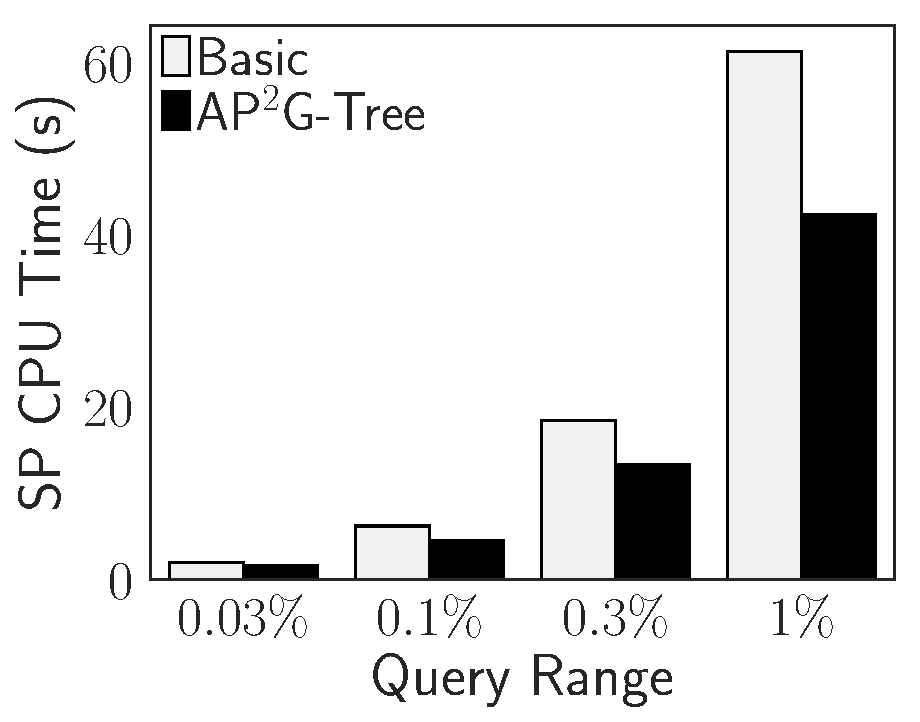
\includegraphics[width=\linewidth]{exp-figs/access-control/range_sp.pdf}
        \caption{SP CPU Time}
    \end{subfigure}~%
    \begin{subfigure}{.33\linewidth}
        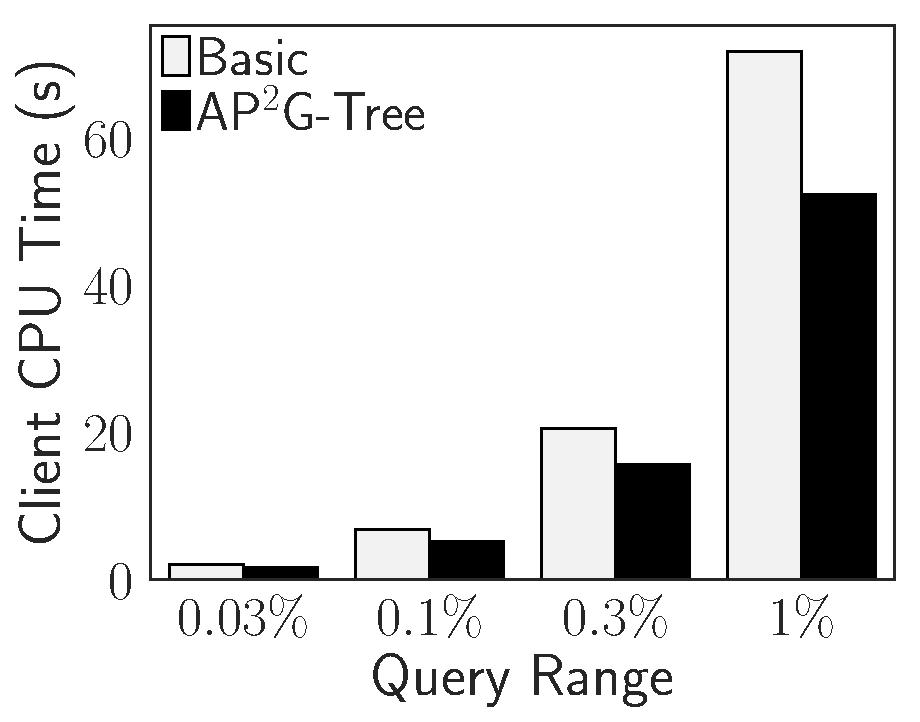
\includegraphics[width=\linewidth]{exp-figs/access-control/range_user.pdf}
        \caption{Client CPU Time}
    \end{subfigure}~%
    \begin{subfigure}{.33\linewidth}
        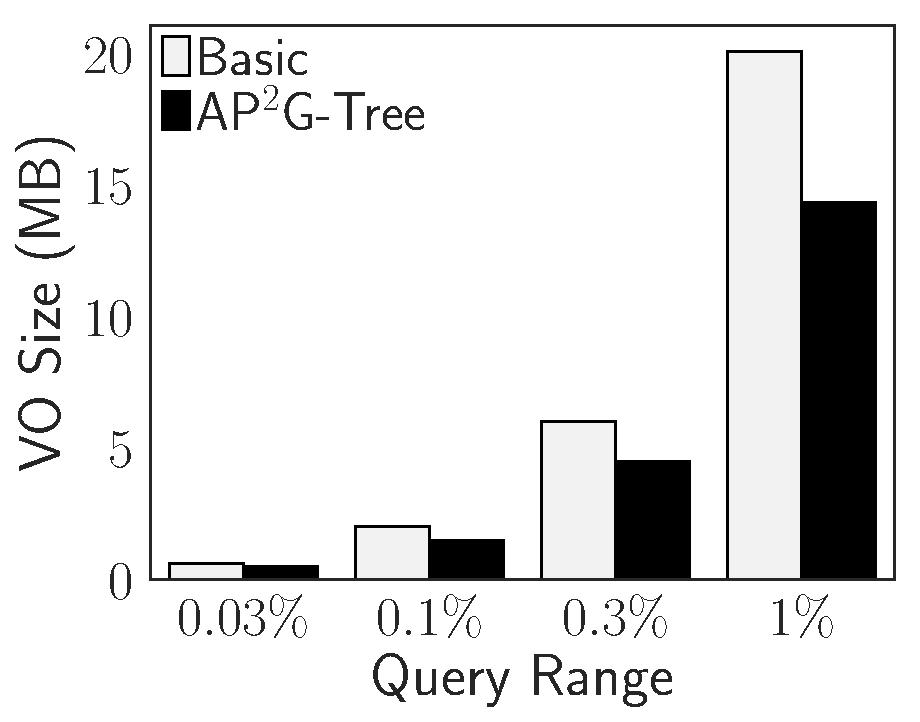
\includegraphics[width=\linewidth]{exp-figs/access-control/range_vo.pdf}
        \caption{VO Size}
    \end{subfigure}
    \caption{Range Query Performance vs. Range}\label{exp-fig:access-control:range}
\end{figure}
\begin{figure}[t]
    \centering
    \begin{subfigure}{.33\linewidth}
        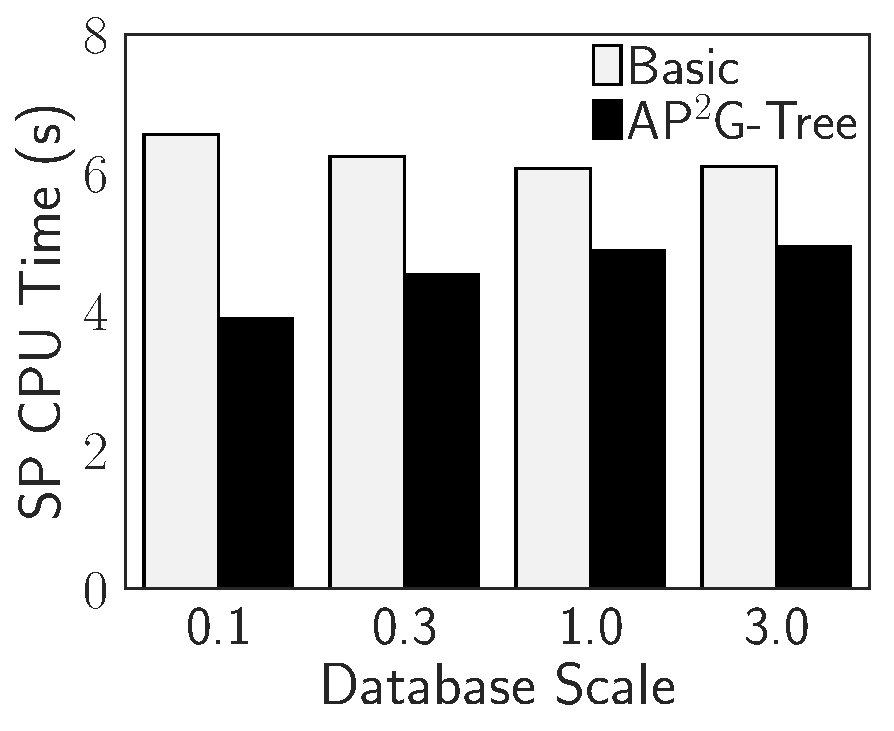
\includegraphics[width=\linewidth]{exp-figs/access-control/scale_sp.pdf}
        \caption{SP CPU Time}
    \end{subfigure}~%
    \begin{subfigure}{.33\linewidth}
        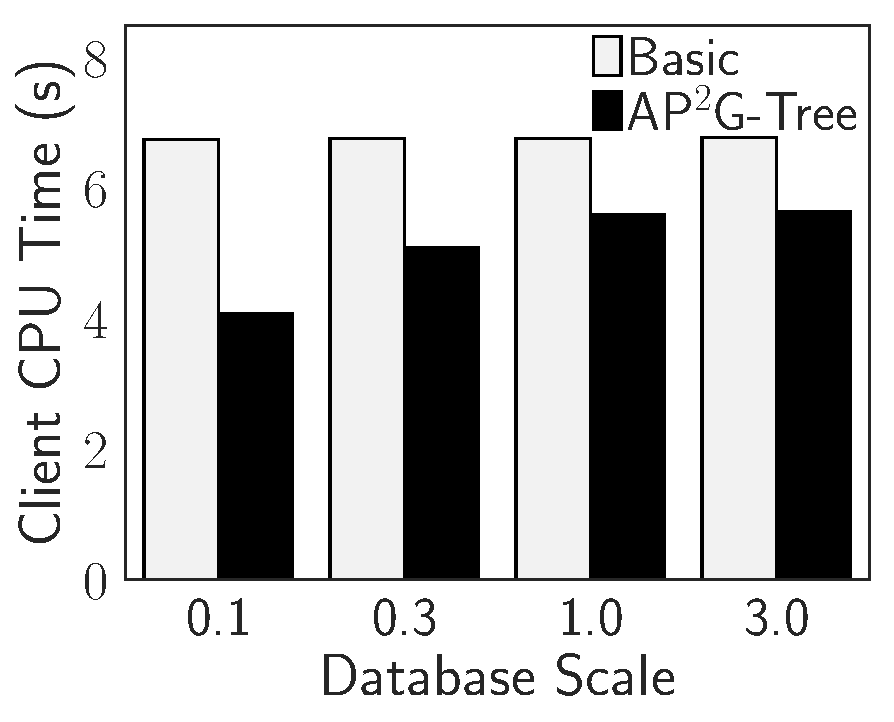
\includegraphics[width=\linewidth]{exp-figs/access-control/scale_user.pdf}
        \caption{Client CPU Time}
    \end{subfigure}~%
    \begin{subfigure}{.33\linewidth}
        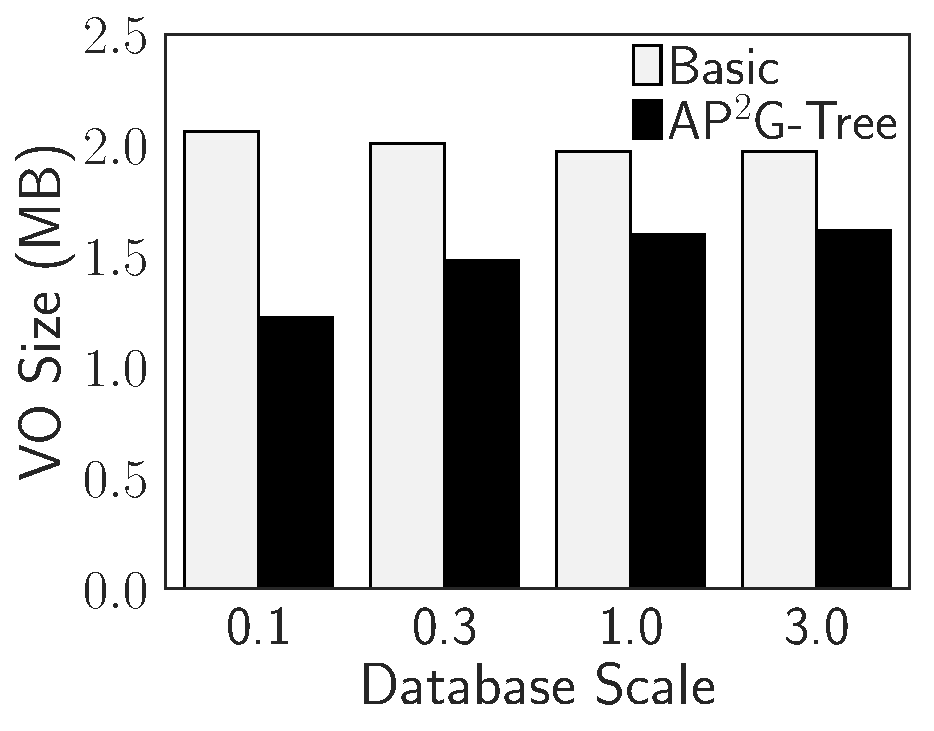
\includegraphics[width=\linewidth]{exp-figs/access-control/scale_vo.pdf}
        \caption{VO Size}\label{exp-fig:scale_vo}
    \end{subfigure}
    \caption{Range Query Performance vs. Database Scale}\label{exp-fig:access-control:scale}
\end{figure}
\begin{figure}[t]
    \centering
    \begin{subfigure}{.33\linewidth}
        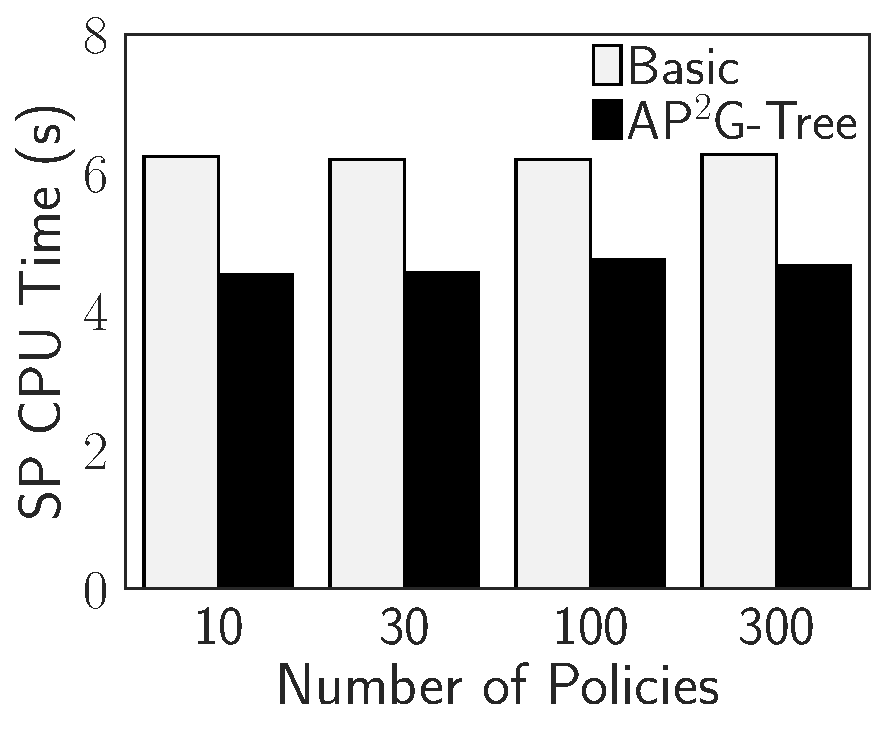
\includegraphics[width=\linewidth]{exp-figs/access-control/policy_1_sp.pdf}
        \caption{SP CPU Time}
    \end{subfigure}~%
    \begin{subfigure}{.33\linewidth}
        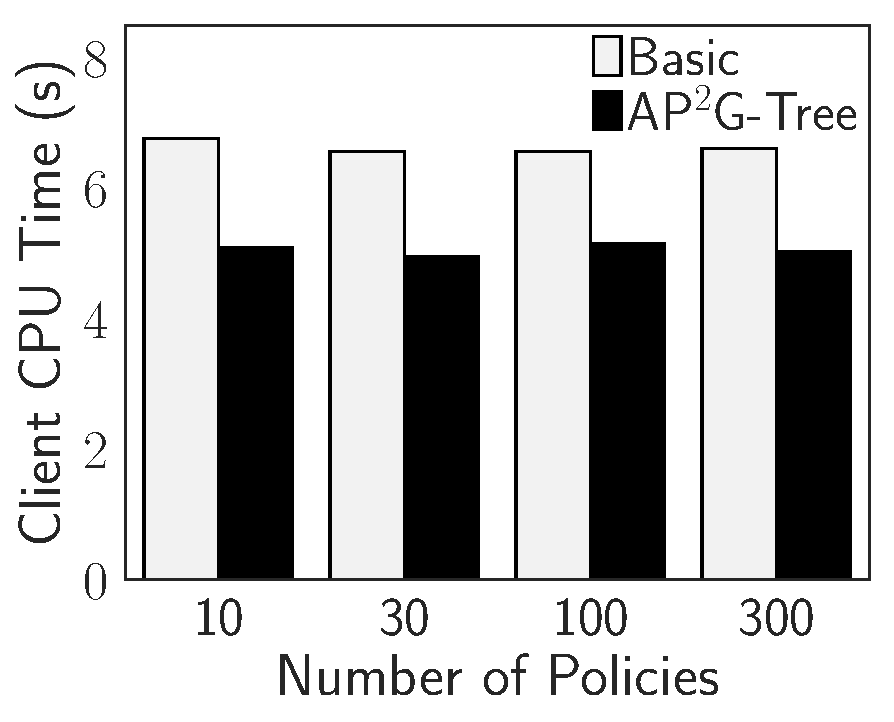
\includegraphics[width=\linewidth]{exp-figs/access-control/policy_1_user.pdf}
        \caption{Client CPU Time}
    \end{subfigure}~%
    \begin{subfigure}{.33\linewidth}
        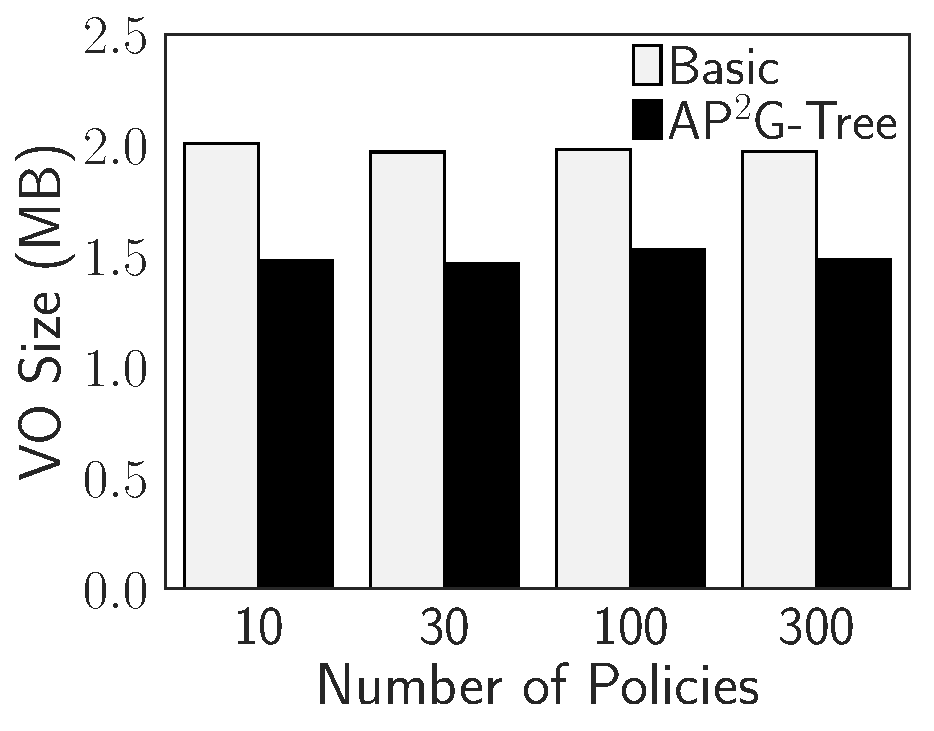
\includegraphics[width=\linewidth]{exp-figs/access-control/policy_1_vo.pdf}
        \caption{VO Size}
    \end{subfigure}
    \caption{Range Query Performance vs. Policy Diversity}\label{exp-fig:access-control:policy_1}
\end{figure}
\begin{figure}[t]
    \centering
    \begin{subfigure}{.33\linewidth}
        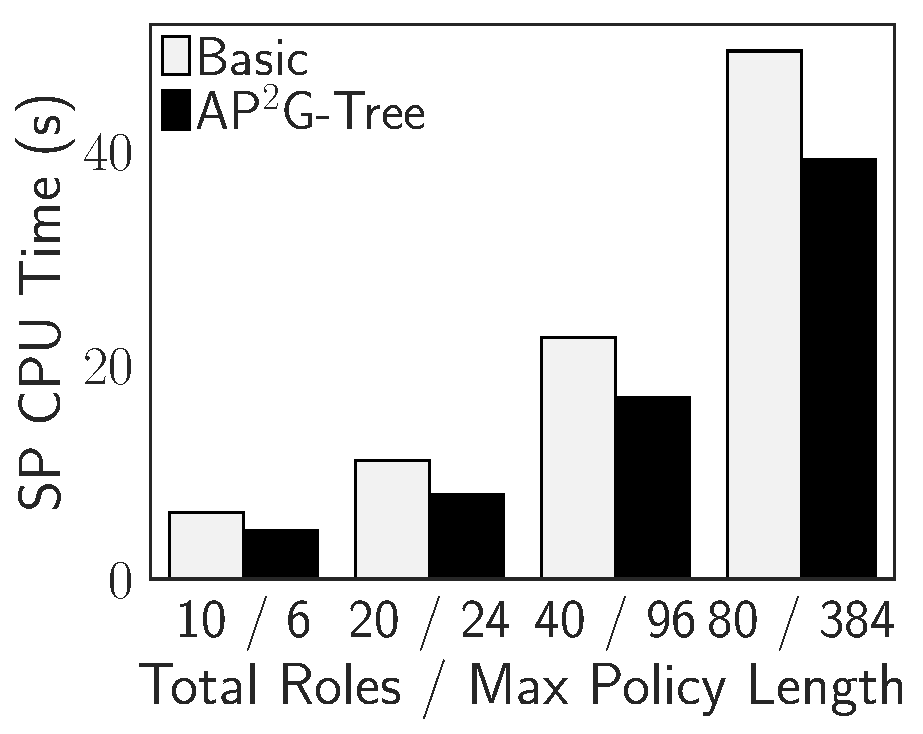
\includegraphics[width=\linewidth]{exp-figs/access-control/policy_2_sp.pdf}
        \caption{SP CPU Time}
    \end{subfigure}~%
    \begin{subfigure}{.33\linewidth}
        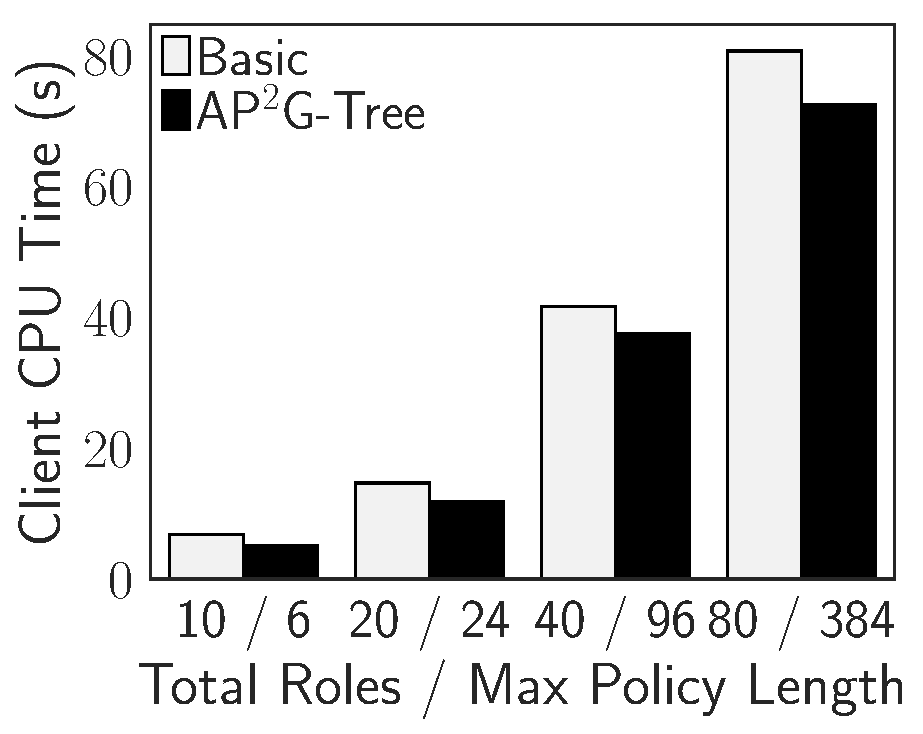
\includegraphics[width=\linewidth]{exp-figs/access-control/policy_2_user.pdf}
        \caption{Client CPU Time}
    \end{subfigure}~%
    \begin{subfigure}{.33\linewidth}
        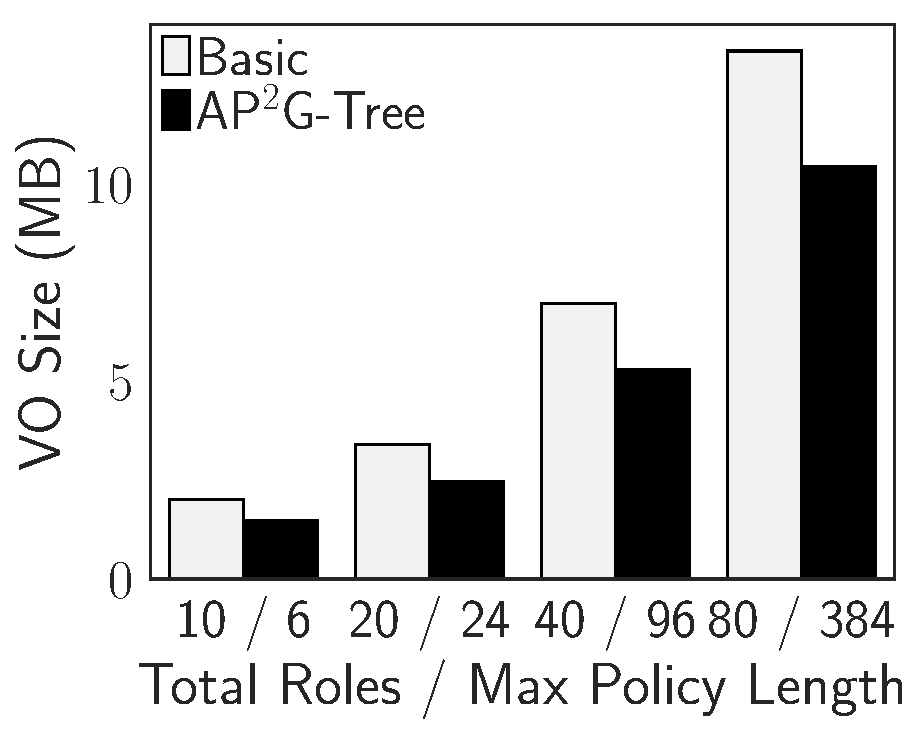
\includegraphics[width=\linewidth]{exp-figs/access-control/policy_2_vo.pdf}
        \caption{VO Size}
    \end{subfigure}
    \caption{Range Query Performance vs. Total Roles}\label{exp-fig:access-control:policy_2}
\end{figure}
\begin{figure}[t]
    \centering
    \begin{subfigure}{.33\linewidth}
        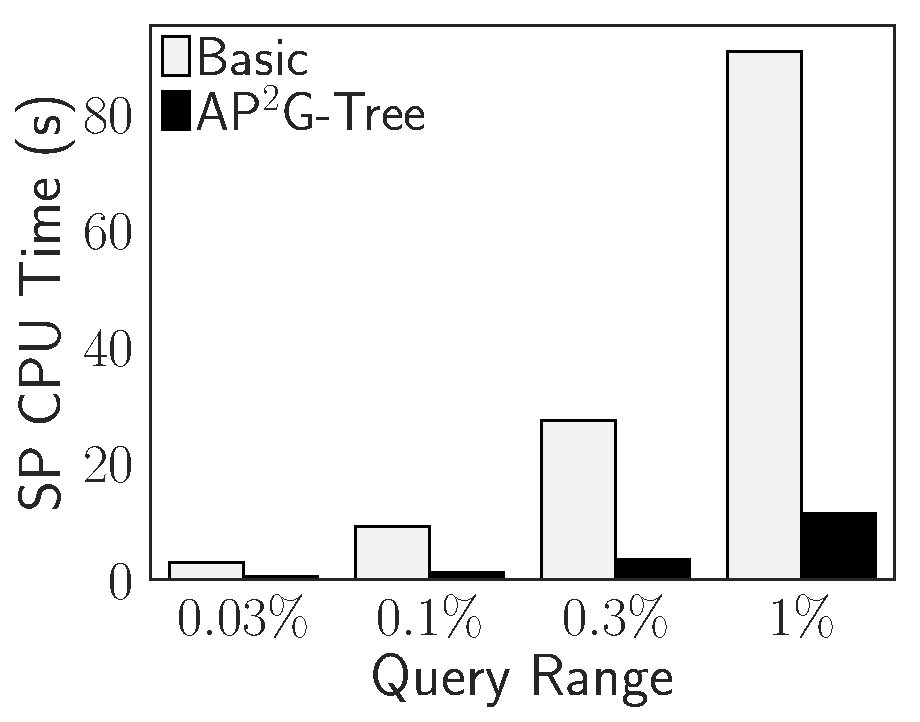
\includegraphics[width=\linewidth]{exp-figs/access-control/join_sp.pdf}
        \caption{SP CPU Time}
    \end{subfigure}~%
    \begin{subfigure}{.33\linewidth}
        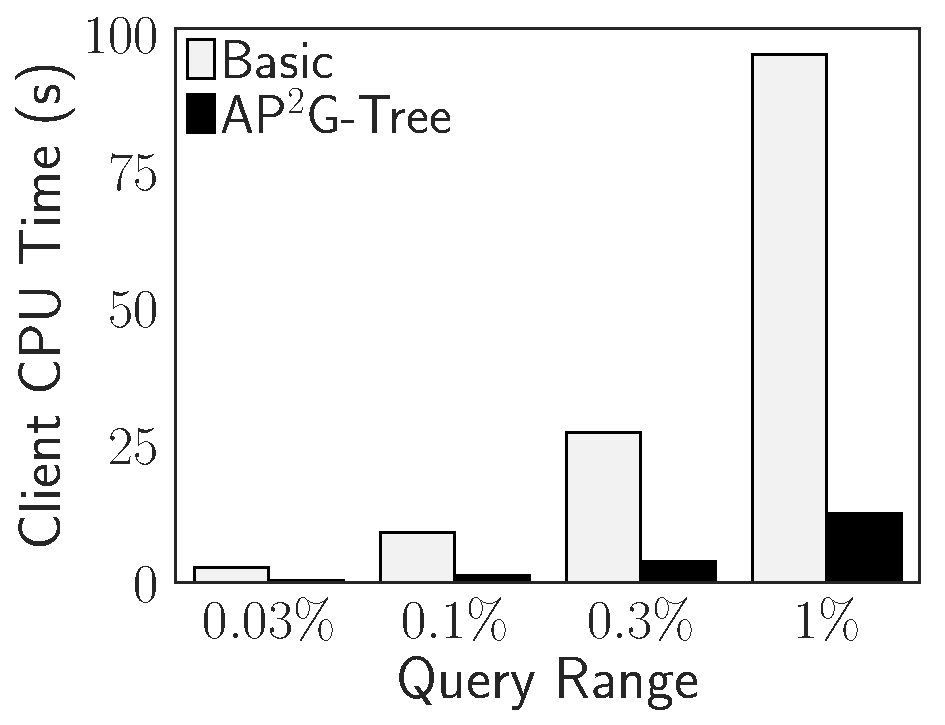
\includegraphics[width=\linewidth]{exp-figs/access-control/join_user.pdf}
        \caption{Client CPU Time}
    \end{subfigure}~%
    \begin{subfigure}{.33\linewidth}
        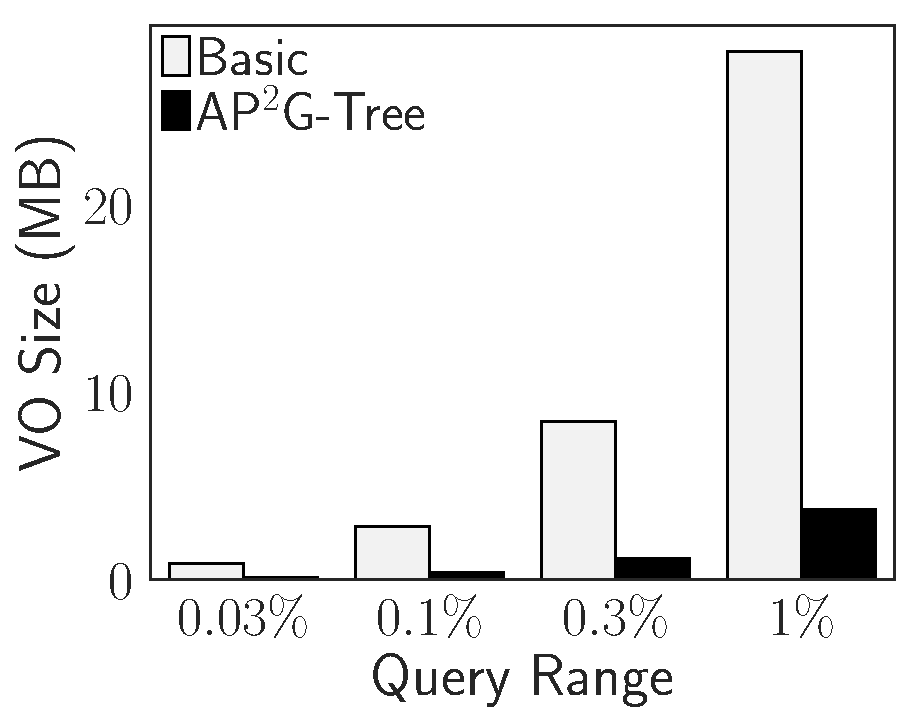
\includegraphics[width=\linewidth]{exp-figs/access-control/join_vo.pdf}
        \caption{VO Size}
    \end{subfigure}
    \caption{Join Query Performance vs. Range}\label{exp-fig:access-control:join}
\end{figure}

To evaluate the range query authentication performance, we compare two methods:
\begin{inlineenum}
    \item the basic approach in which equality query authentication is executed repeatedly for every discrete value lying in the query range, and
    \item the AP$^2$G-tree approach developed in \Cref{sec:access-control:range-query}.
\end{inlineenum}
In each query, the client is assigned with the roles that can access 20\% of the data records.

We first vary the query range from 0.03\% to 1\% of the data space under the default settings. As shown in \Cref{exp-fig:access-control:range}, the AP$^2$G-tree outperforms the basic approach in all metrics. This indicates that the APS signatures generated for AP$^2$G-tree nodes can effectively summarize the inaccessible records in their subtrees. This leads to the reduction in both computation and communication overheads.

To investigate the impact of the database scale and access policies, we fix the query range at 0.1\%. \Cref{exp-fig:access-control:scale} shows the results when the database scale is varied from 0.1 to 3. All metrics increase monotonically under AP$^2$G-tree, but those of the basic approach fluctuate a bit. This can be explained as follows. With more records, the access policies become more complex. This affects the costs in two ways:
\begin{inlineenum}
    \item it takes the SP more time to process the \textsf{ABS.Relax} operations, and
    \item it takes the client more time to verify the APP signatures.
\end{inlineenum}
On the other hand, with the increase of database scale, more records can be accessed by the client and, hence, the inaccessible records become fewer. This decreases the costs on both the SP and the client.
For AP$^2$G-tree, owing to its high pruning power, the decreased number of inaccessible records has less impact on the costs. Therefore, its costs increase steadily.

\Cref{exp-fig:access-control:policy_1} and~\Cref{exp-fig:access-control:policy_2} show the performance trends with the respect to the number of distinct policies and the total number of roles/max policy length, respectively. It can be seen that the performance remains almost the same under different policy diversities. However, the larger the role space and the longer access policy length, the higher the overhead incurred for both the computation and communication costs.

Finally, to study the join query performance, we evaluate the join operator of $Q$12 in TPC-H,\footnote{\texttt{SELECT * FROM orders, lineitem WHERE o.orderkey = l.orderkey AND l.orderkey between `?' AND `?'.}} which joins the tables \texttt{Lineitem} and \texttt{Orders} on the attribute $orderkey$. \Cref{exp-fig:access-control:join} reports the results while varying the query range. It is shown that the costs in all metrics under AP$^2$G-tree are substantially lower than those in the basic approach.

\subsection{Impact of the Optimizations}

\begin{figure}[t]
    \centering
    \begin{subfigure}{.33\linewidth}
        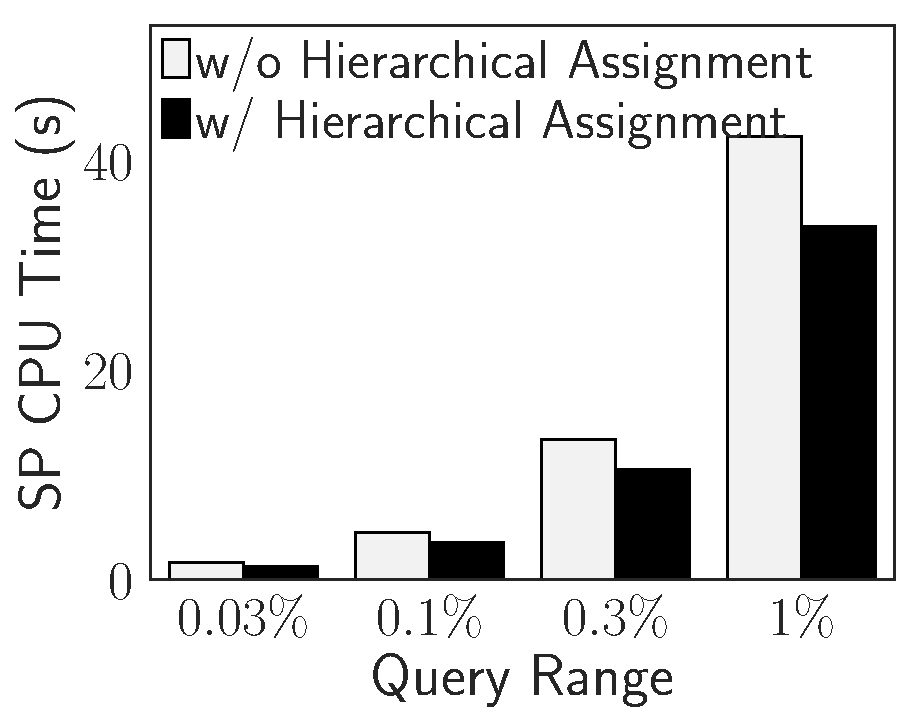
\includegraphics[width=\linewidth]{exp-figs/access-control/hierarchical_sp.pdf}
        \caption{SP CPU Time}
    \end{subfigure}~%
    \begin{subfigure}{.33\linewidth}
        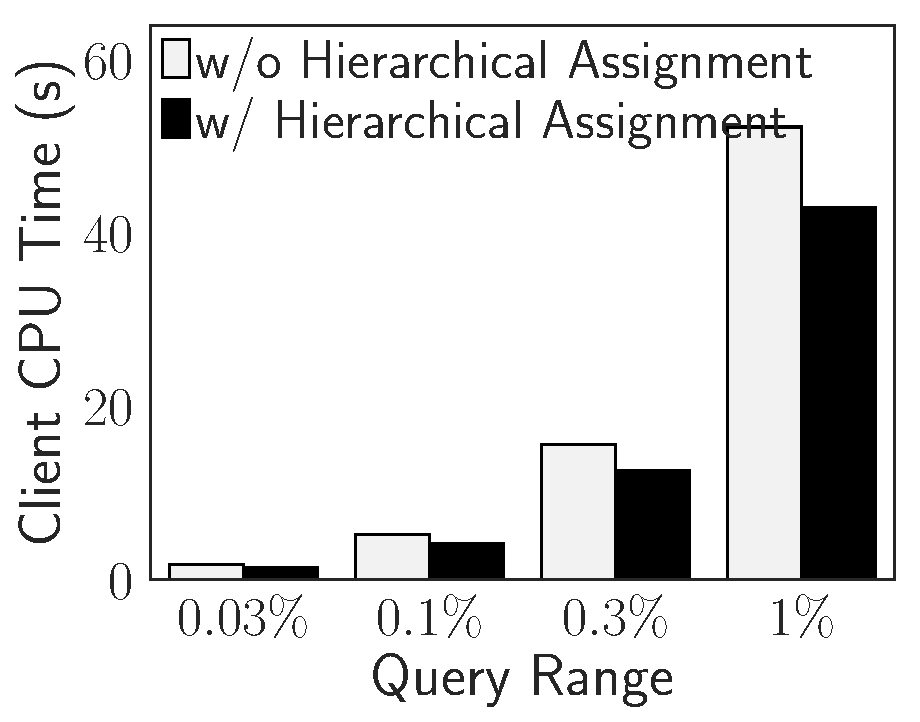
\includegraphics[width=\linewidth]{exp-figs/access-control/hierarchical_user.pdf}
        \caption{Client CPU Time}
    \end{subfigure}~%
    \begin{subfigure}{.33\linewidth}
        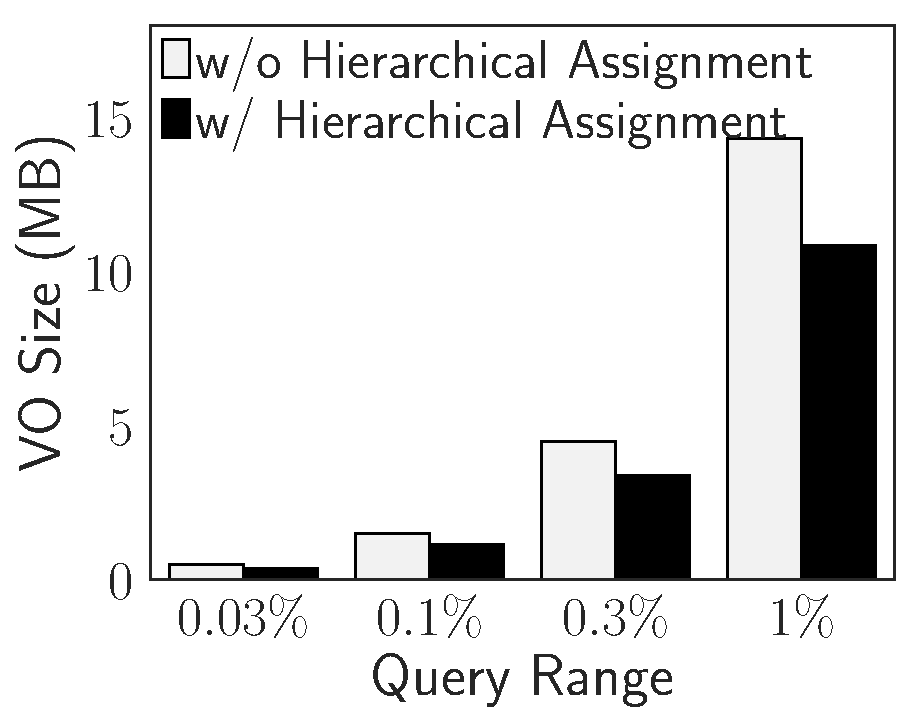
\includegraphics[width=\linewidth]{exp-figs/access-control/hierarchical_vo.pdf}
        \caption{VO Size}
    \end{subfigure}
    \caption{Hierarchical Role Assignment Acceleration}\label{exp-fig:access-control:hierarchical}
\end{figure}
\begin{figure}[t]
    \centering
    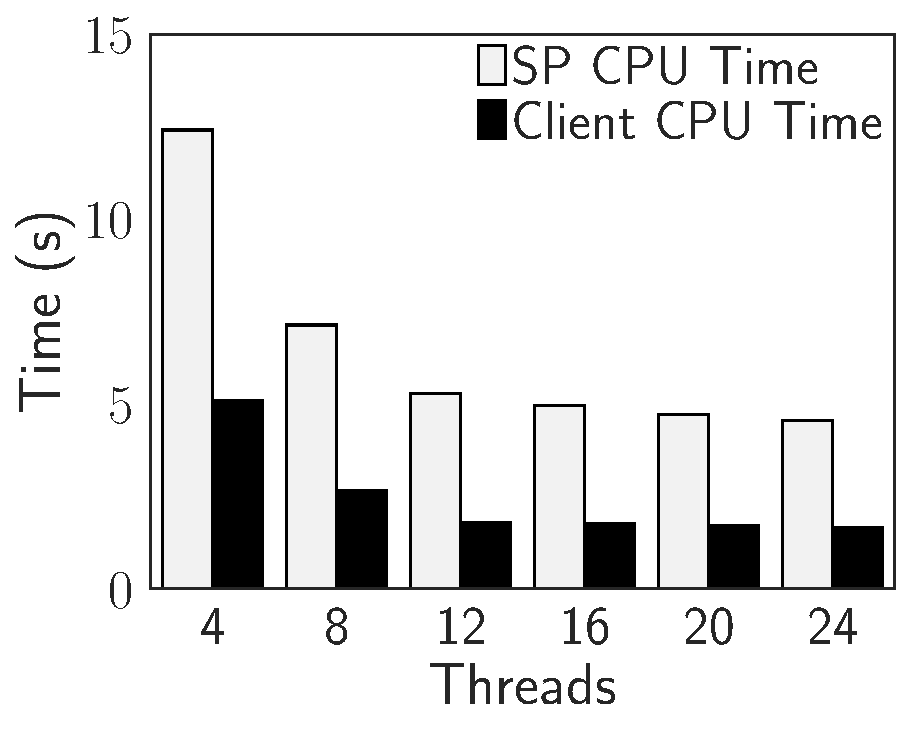
\includegraphics[width=0.33\linewidth]{exp-figs/access-control/thread.pdf}
    \caption{Multi-Threaded Acceleration}\label{exp-fig:access-control:thread}
\end{figure}
\begin{figure}[t]
    \centering
    \begin{subfigure}{.33\linewidth}
        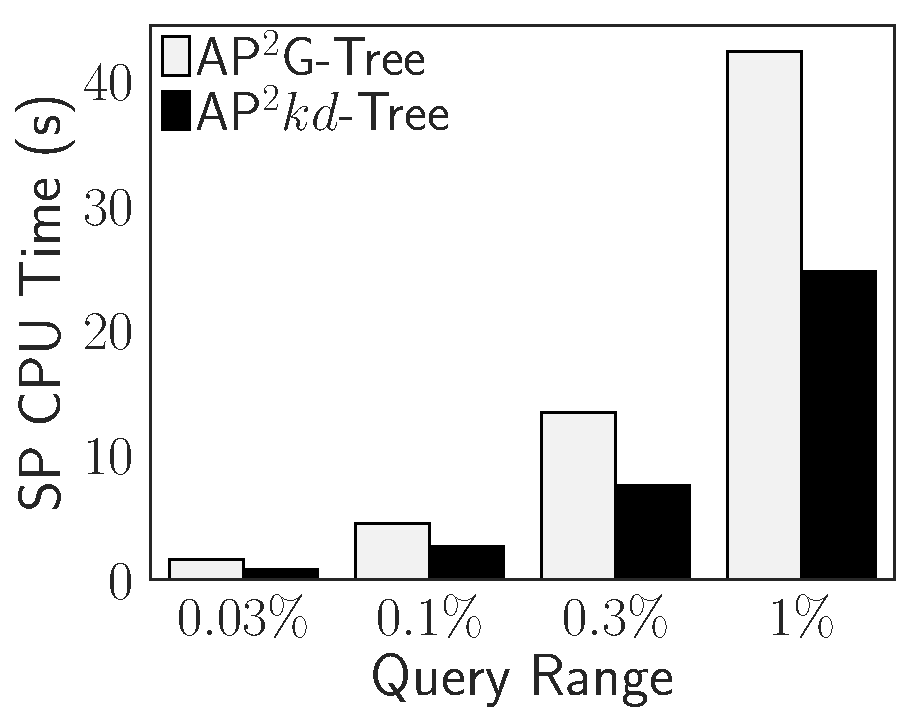
\includegraphics[width=\linewidth]{exp-figs/access-control/index_1_sp.pdf}
        \caption{SP CPU Time}
    \end{subfigure}~%
    \begin{subfigure}{.33\linewidth}
        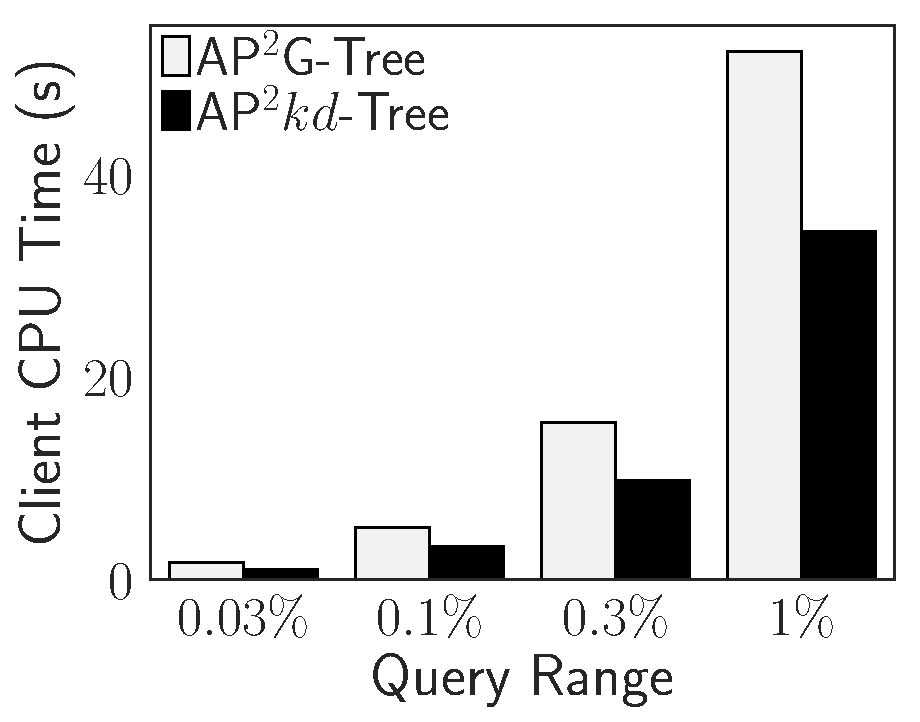
\includegraphics[width=\linewidth]{exp-figs/access-control/index_1_user.pdf}
        \caption{Client CPU Time}
    \end{subfigure}~%
    \begin{subfigure}{.33\linewidth}
        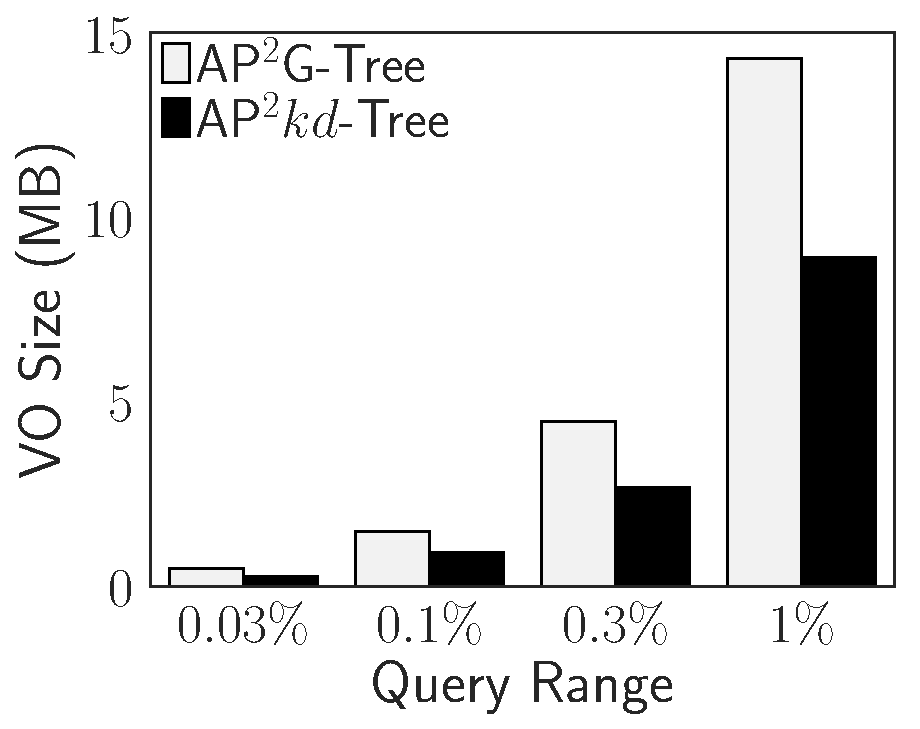
\includegraphics[width=\linewidth]{exp-figs/access-control/index_1_vo.pdf}
        \caption{VO Size}
    \end{subfigure}
    \caption{Range Query Performance vs. Index}\label{exp-fig:access-control:index}
\end{figure}

We now investigate the impact of different optimization techniques proposed in \Cref{sec:access-control:opt}. The results of using hierarchical role assignment are shown in \Cref{exp-fig:access-control:hierarchical}. In our experiment, we simulate a two-level role hierarchy. Two global hierarchical roles are created and attached randomly to each AND gate in all the access policies. As a result, the average size of a client's inaccessible predicate is decreased from 9 to 6. It can be observed that the hierarchical role assignment reduces the cost in all metrics, due to much less overhead in processing inaccessible records.

To study the acceleration acquired by parallelism, we vary the number of threads for both the SP processing and client verification running on the blade server. As shown in \Cref{exp-fig:access-control:thread}, more acceleration can be observed with the first 16 threads, but it becomes less effective with more threads. The reason is that the non-parallel part of the algorithm and I/O operations becomes more pronounced after sufficient multi-thread acceleration.

Finally, we study the performance gain if we relax the zero-knowledge confidentiality requirement. As shown in \Cref{exp-fig:access-control:index}, owing to a careful splitting strategy introduced in \Cref{sec:access-control:kd-tree}, AP$^2kd$-tree substantially outperforms AP$^2$G-tree in all evaluation metrics.

\subsection{Performance with Duplicate Records and Updates}

\begin{figure}[t]
    \centering
    \begin{subfigure}{.33\linewidth}
        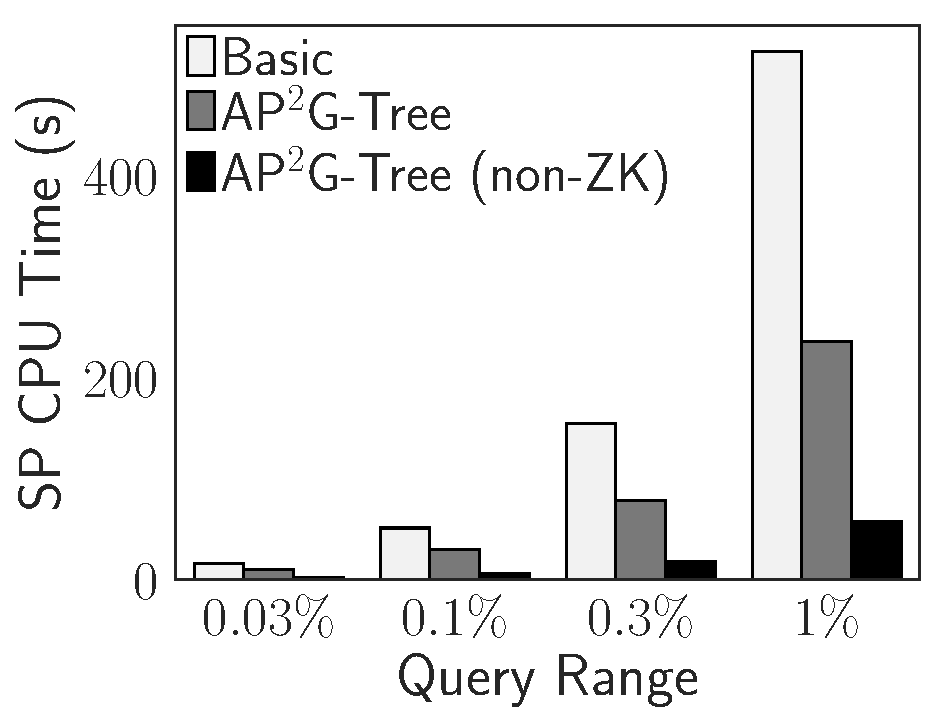
\includegraphics[width=\linewidth]{exp-figs/access-control/dup_sp.pdf}
        \caption{SP CPU Time}
    \end{subfigure}~%
    \begin{subfigure}{.33\linewidth}
        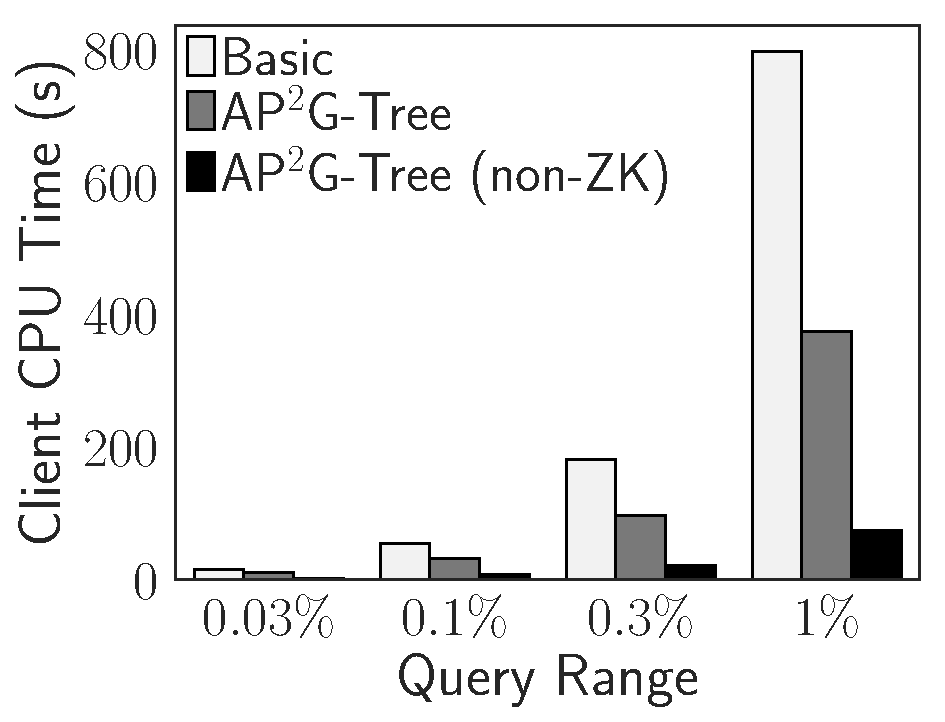
\includegraphics[width=\linewidth]{exp-figs/access-control/dup_user.pdf}
        \caption{Client CPU Time}
    \end{subfigure}~%
    \begin{subfigure}{.33\linewidth}
        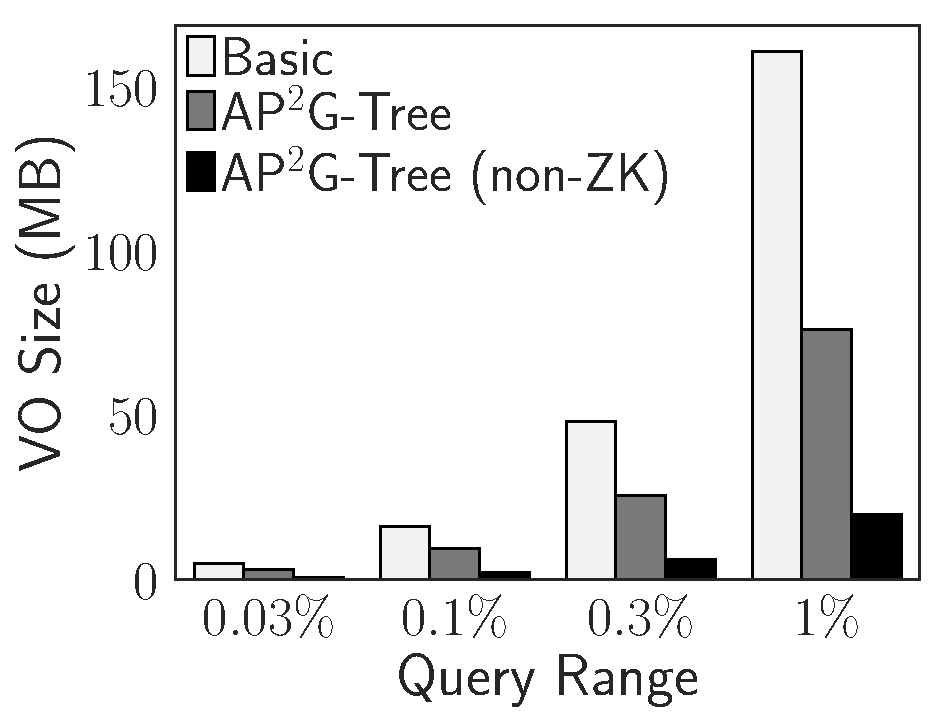
\includegraphics[width=\linewidth]{exp-figs/access-control/dup_vo.pdf}
        \caption{VO Size}
    \end{subfigure}
    \caption{Range Query Performance with Duplicate Records}\label{exp-fig:access-control:dup}
\end{figure}

To investigate the performance with duplicate records using methods proposed in \Cref{sec:access-control:dup}, we conduct performance evaluation over the default TPC-H database, where the access policies are randomly assigned to all data records.
We compare two solutions of handling duplicate records:
\begin{inlineenum}
    \item the zero-knowledge approach by adding the virtual dimension (denoted as AP$^2$G-Tree);
    \item the non-zero-knowledge approach by embedding the duplicate information in the APP signatures (denoted as AP$^2$G-Tree (non-ZK)).
\end{inlineenum}
The index size for the zero-knowledge approach is 12.17 GB (2.91 GB tree structure + 9.26 GB signatures), whereas in the non-zero-knowledge setting the index is 4.35 GB (1.02 GB tree structure + 3.33 GB signatures). The additional index overhead incurred for the zero-knowledge approach, as the cost of achieving the zero-knowledge requirement, is believed to be reasonable. Regarding the query performance, AP$^2$G-Tree (non-ZK) is approximate to the case without duplicate records since the duplicate information is seamlessly embedded in the APP signatures. As shown in \Cref{exp-fig:access-control:dup}, the query cost in the zero-knowledge AP$^2$G-tree approach is only no more than 3 times worse than that in AP$^2$G-Tree (non-ZK). Moreover, the performance of AP$^2$G-tree is only about half that of the basic approach, which again demonstrates its pruning effectiveness for inaccessible records.

\begin{figure}[t]
    \centering
    \begin{subfigure}[b]{.4\linewidth}
        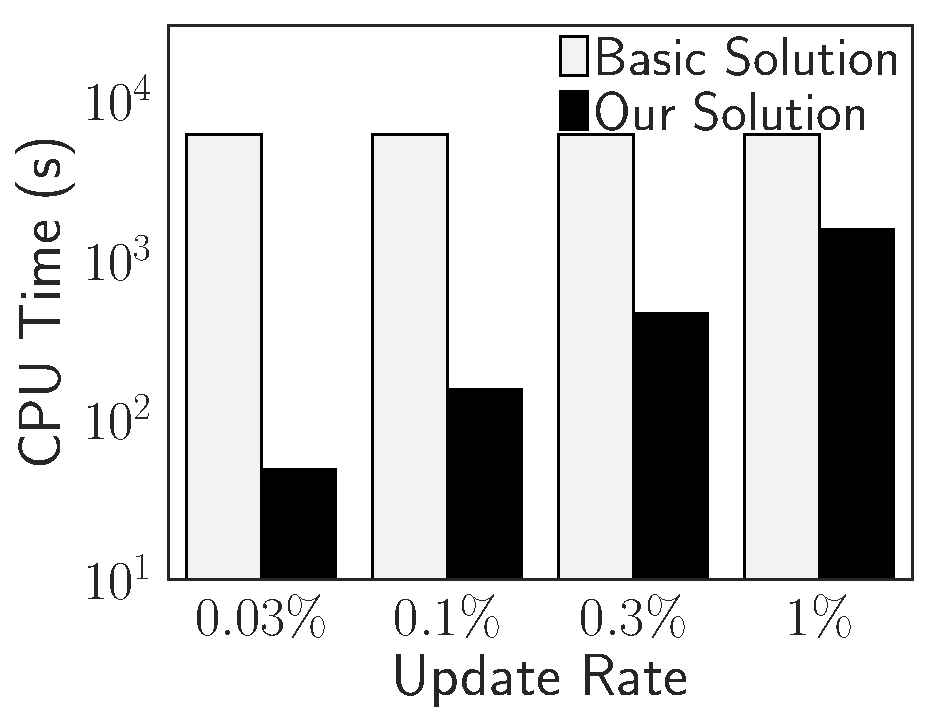
\includegraphics[width=\linewidth]{exp-figs/access-control/update_do_time.pdf}
        \caption{DO CPU Time}\label{exp-fig:access-control:update_do_time}
    \end{subfigure}~%
    \begin{subfigure}[b]{.4\linewidth}
        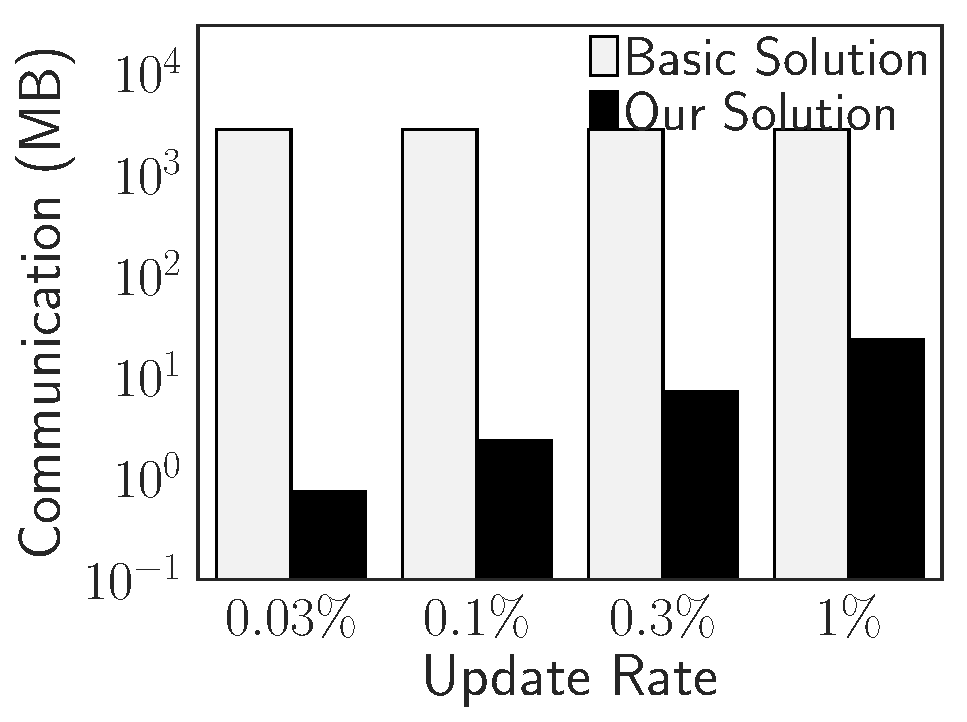
\includegraphics[width=\linewidth]{exp-figs/access-control/update_do_size.pdf}
        \caption{Communication Cost}\label{exp-fig:access-control:update_do_size}
    \end{subfigure}~%
    \caption{Update Performance vs. Update Rate}\label{exp-fig:access-control:update_do}
\end{figure}
\begin{figure}[t]
    \centering
    \begin{subfigure}{.33\linewidth}
        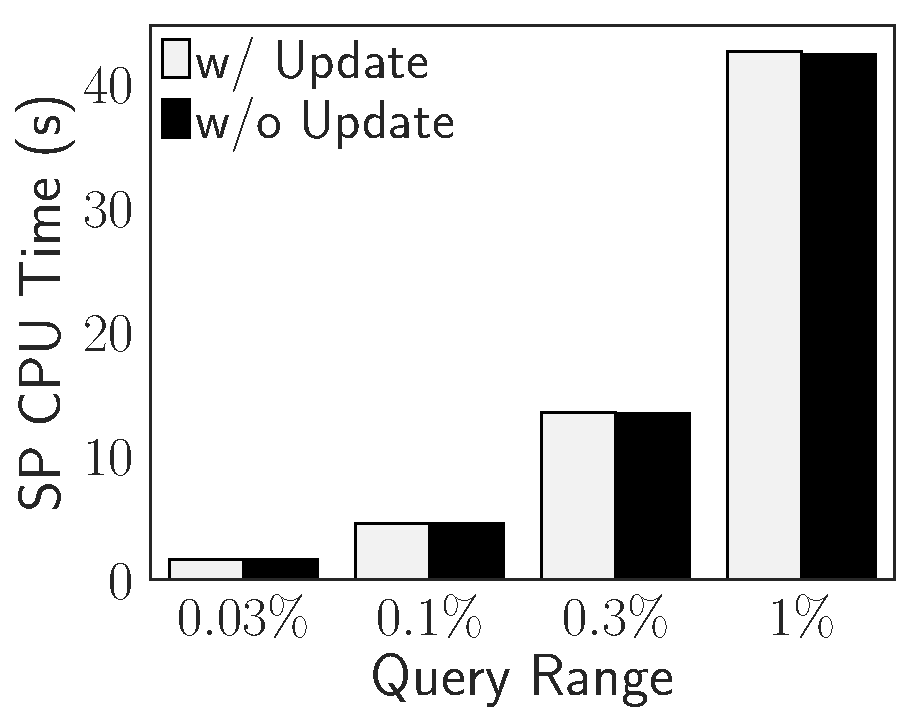
\includegraphics[width=\linewidth]{exp-figs/access-control/update_sp.pdf}
        \caption{SP CPU Time}
    \end{subfigure}~%
    \begin{subfigure}{.33\linewidth}
        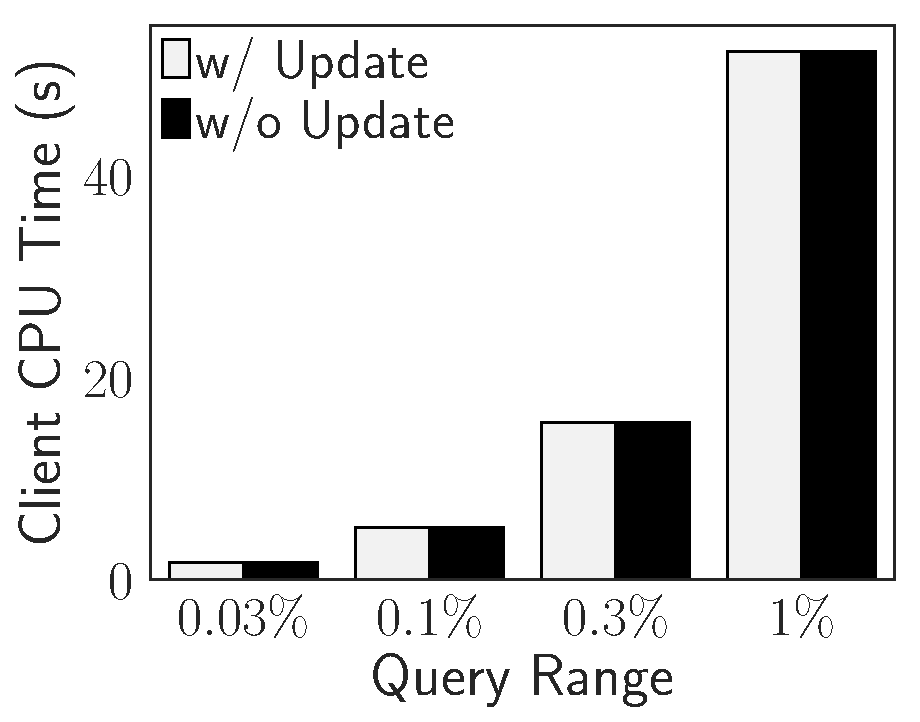
\includegraphics[width=\linewidth]{exp-figs/access-control/update_user.pdf}
        \caption{Client CPU Time}
    \end{subfigure}~%
    \begin{subfigure}{.33\linewidth}
        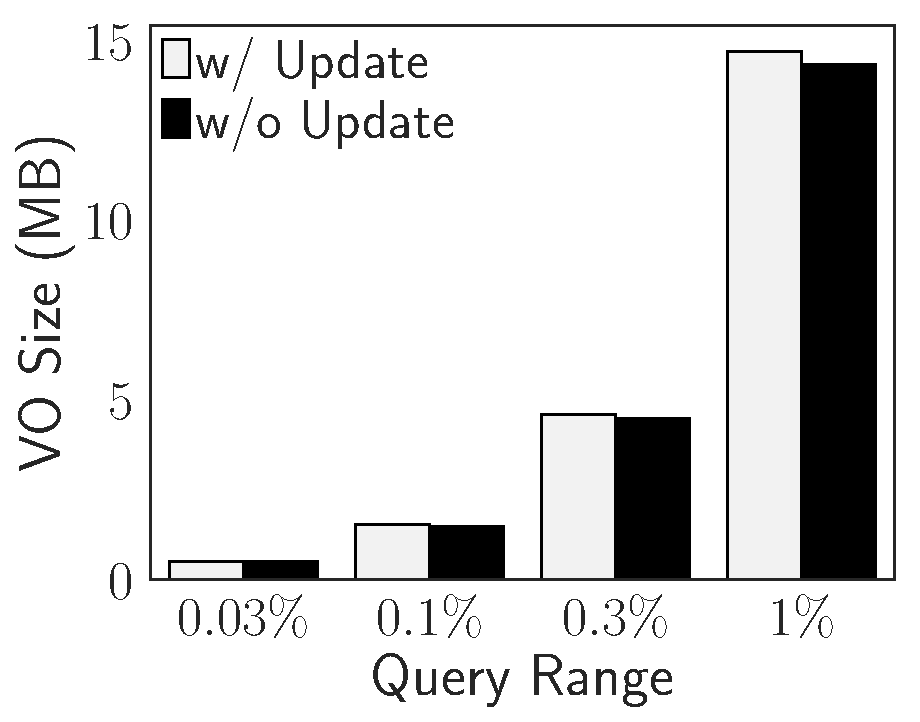
\includegraphics[width=\linewidth]{exp-figs/access-control/update_vo.pdf}
        \caption{VO Size}
    \end{subfigure}
    \caption{Range Query Performance vs. Update}\label{exp-fig:access-control:update}
\end{figure}

Finally, we conduct an empirical study over the default TPC-H database to evaluate the performance of our update strategy proposed in \Cref{sec:access-control:update}. We compare two update methods:
\begin{inlineenum}
    \item the basic approach in which the DO resigns all of the APP signatures; and
    \item our proposed solution described above.
\end{inlineenum}
\Cref{exp-fig:access-control:update_do} reports the DO CPU time and the communication cost while varying the update rate from $0.03\%$ to $1\%$ of all the records. It can be observed that our solution is significantly better than the basic approach. Further, we study the performance differences of authenticating range queries with and without data record updates. As shown in \Cref{exp-fig:access-control:update}, the differences in all metrics are insignificant.

\section{Chapter Summary}\label{sec:access-control:summary}
In this chpater, we have studied the problem of authenticating relational queries with fine-grained access control. We developed a new variant of the attribute-based signature scheme, which supports predicate relaxation on super access policies. Based on that, we proposed a novel access-policy-preserving (APP) signature as the primitive ADS to authenticate various types of queries under fine-grained access control. Our approach is zero-knowledge and reveals nothing beyond the accessible records. We also designed a grid-index-based AP$^2$G-tree to improve the performance of processing range queries and join queries. Optimization techniques for both the zero-knowledge model and the access policy confidentiality model were developed. Analytical models and empirical results substantiated the robustness and efficiency of our proposed solutions.
%
\chapter{Authenticating {kNN} Queries in Distributed Environment}\label{chap:knn}

In this chapter, we investigate the problem of authenticating {kNN} queries in distributed environment.

\section{Problem Formulation}\label{sec:knn:problem}

There are three parties in our system: the DO, the third-party distributed SP, and the client. The DO builds the ADS and signs the ADS to ensure the integrity of the data. The ADS and the signature are then sent to the SP\@. The distributed SP provides the service of storage and query processing. Since the SP is configured in a distributed environment, it consists of several types of nodes: $Master$, $Slave$, and $Reducer$. The $Master$ node in the SP is mainly responsible for dispatching jobs to the corresponding slaves. The $Slave$ nodes are the workers, which process the actual queries. The $Reducer$ consolidates all the partial results as well as the VOs computed by the $Slaves$ and sends them to the client. Finally, the client can verify the soundness and completeness of the results by using the VO, the DO's public key, and the root signature sent by the SP\@.

\textbf{Threat Model.}
In this system, we consider the DO as the trusted party. The SP is untrusted and can return incorrect results. Given the whole dataset $D$, the client's query point $q$, and the parameter $k$, the SP returns several results. If the result number does not match the value $k$, the client can find that some results are missing. Suppose $R_{k}=\{r_{1},r_{2},\dots,r_{k}\}$ are the $k$ true kNN results. The SP can
\begin{inlineenum}
\item return a point $p$ and $p \notin D$;
\item return a point $p \in D$ but $dist(q,p) > dist(q,r_{k})$, where $dist(\cdot,\cdot)$ denotes the Euclidean distance.
\end{inlineenum}
The first and second cases violate the soundness and completeness conditions, respectively.

The system's performance can be measured in these metrics:
\begin{inlineenum}
\item ADS construction time;
\item query processing cost;
\item client's verification time; and
\item VO size.
\end{inlineenum}
We assume that there is no data update in this system. Therefore, the ADS construction is a one-off operation by the DO and the cost can be amortized by the queries. The VO size can influence the communication overhead between the SP and the client as well as the time of client's verification. Therefore, the VO size should be minimized.

\section{Preliminaries}\label{sec:knn:prelim}

\subsection{Cryptographic Primitives}

In our solution, two cryptographic primitives are used, namely hash function and digital signature.

\textbf{Hash Function}: A one-way hash function $H(\cdot)$ transforms an arbitrary message $m$ to a fixed-length digest $H(m)$. One-way indicates that given a message $m$, the computation of $H(m)$ is easy. However, to get $m$ from $H(m)$ is computationally infeasible. In this chapter, we use SHA-1 as the hash function, which maps a given message to a 160-bit digest.

\textbf{Digital Signature}: The asymmetric signature is used to verify the integrity of the data. The DO keeps a private key and publishes the corresponding public key to the verifier. The DO signs the data using the private key and the verifier can verify the signature using the public key to ensure the integrity of the data. RSA is one of the popular asymmetric signature algorithms.

\subsection{Spatial Authenticated Data Structure}

MR-tree~\cite{10.1007/s00778-008-0113-2}, which is the combination of the R-tree and the Merkle Hash tree~\cite{10.1007/0-387-34805-0_21}, is often used to process authenticated spatial queries. Each leaf node stores the pointers pointing to the data points and the hash value of the binary concatenation of the data points. The hash value of an internal node is computed by hashing the concatenation of each child node's MBR and hash value. We give an example based on \Cref{fig:knn:local-mrtree}, which depicts the data points and their corresponding MR-tree. The leaf node $N_{3}$'s hash value is $H(a|b|c)$, where `$|$' represents the binary concatenation. The non-leaf node's hash value $H(N_{1})=H(N_{3}|H(N_{3})|N_{4}|H(N_{4}))$. Here $N_{3}, N_{4}$ represent the MBR of node $N_{3}$ and $N_{4}$, respectively. We only show three hash values in \Cref{fig:knn:local-mrtree} and other hash values are computed similarly.

\begin{figure}[t]
  \centering
  \begin{subfigure}[b]{.35\linewidth}
    \centering
    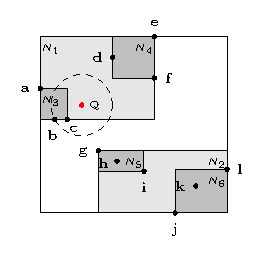
\includegraphics[width=\linewidth]{figs/knn/local-mrtree-data.pdf}
    \caption{Data}\label{fig:knn:local-mrtree:data}
  \end{subfigure}~%
  \begin{subfigure}[b]{.65\linewidth}
    \centering
    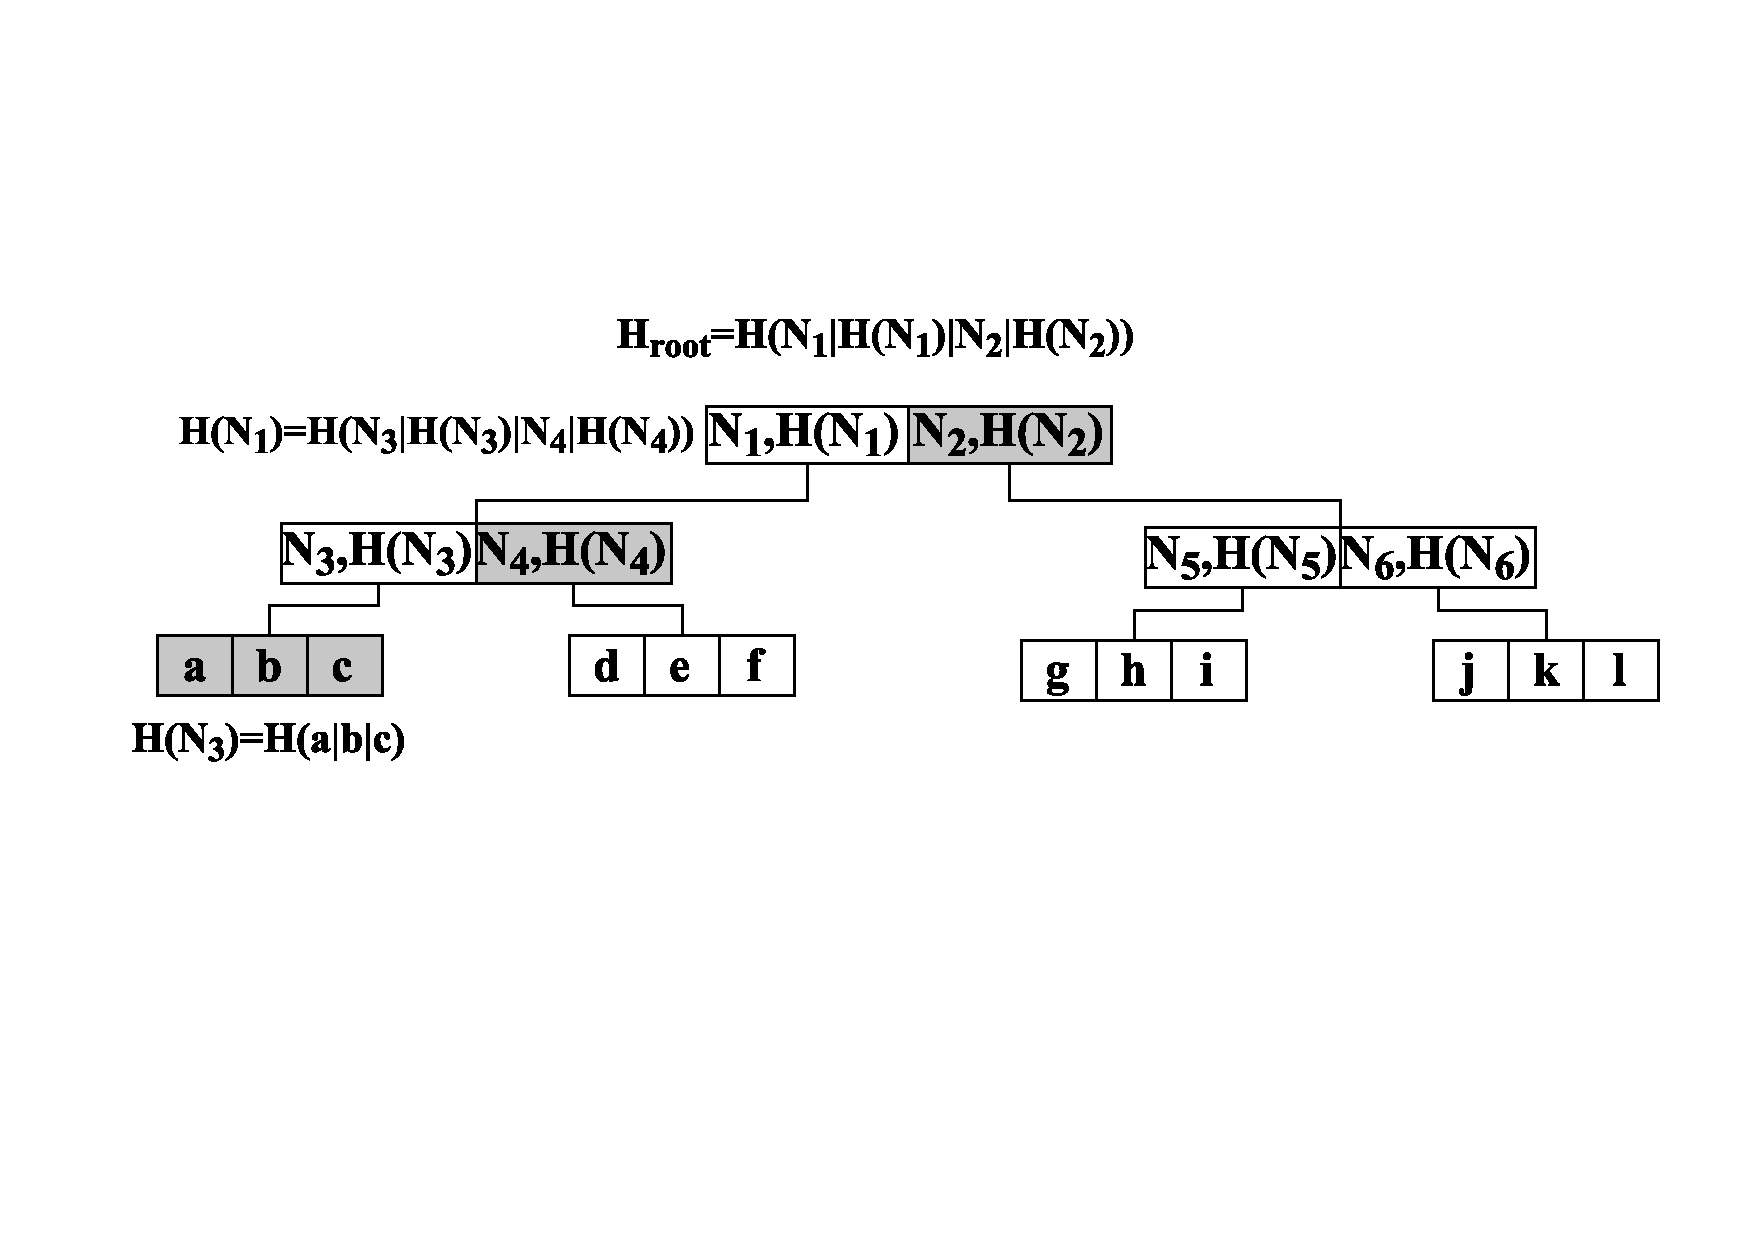
\includegraphics[width=\linewidth]{figs/knn/local-mrtree-tree.pdf}
    \caption{Index}\label{fig:knn:local-mrtree:tree}
  \end{subfigure}
  \caption{Local Authenticated {kNN} Processing}\label{fig:knn:local-mrtree}
\end{figure}

\subsection{Local Authenticated kNN Processing}
There are mainly two different methods of authenticated kNN processing based on the MR-tree. The algorithm proposed by \citeauthor{10.1007/s00778-008-0113-2}~\cite{10.1007/s00778-008-0113-2} mainly focuses on the authenticated range query and transforms the kNN query to a range query. The method separates the generation of the results and the VO\@. It first retrieves kNN results by using any kNN search method. Based on the $k$ results, we can draw a circle centered at the query point $q$ with the radius of the distance between $q$ and the $k^{th}$ result. Then, the authenticated range query is executed to generate the VO set. Another method is to generate the results and the VO set together while traversing the whole MR-tree. \citeauthor{10.1007/978-3-319-18120-2_33}~\cite{10.1007/978-3-319-18120-2_33} proposed the authentication of top-$k$ spatial keyword queries and we can transform this query to the authenticated kNN query easily. \Cref{alg:knn:knn} shows the procedure of generating the VO and results altogether.

\begin{algorithm}[t]
  \caption{Local Authenticated kNN Query}\label{alg:knn:knn}
  \KwIn{$k$, Point $q$, Root of MR-tree $\mathcal{T}_R$}
  \KwOut{Result set $RS$, Verification object $VO$}
  $RS \gets \emptyset$; $counter \gets 0$\;
  $VO \gets (\textrm{`['}, \mathcal{T}_R, \mathcal{T}_R.hash, \textrm{`]'})$\; % chktex 9
  Initialize priority queue $PQ$ and enqueue $\mathcal{T}_R$\;
  \While{$counter < k \land PQ \neq \emptyset$}{%
    $object \gets dequeue(PQ)$\;
    \eIf{$object$ is an MBR $R_i$}{%
      Enqueue each $R_{j}$ or $O_{j}$ in $R_{i}$'s child node into $PQ$\;
      Replace $R_{i}, R_{i}.hash$ with `[', each $R_{j}$, $R_{j}.hash$ (or $O_{j}$) in $R_{i}$'s child node, and `]' in $VO$\;
      }{%
      $RS \gets RS + \{object\}$\;
      $counter \gets counter + 1$\;
    }
  }
  \Return{$\langle RS, VO \rangle$}\;
\end{algorithm}

The algorithm traverses the MR-tree in a best first search manner~\cite{10.1145/320248.320255}. We maintain a priority queue $PQ$. In the while loop, the current nearest object to the point $q$ is dequeued from the priority queue $PQ$. If the object is a node rather than a data point, each of its child node $R_{j}$ will be enqueued to the $PQ$. Otherwise, the object is added to the result set because it is a point. The while loop terminates until $k$ results are collected or the $PQ$ is empty. The VO set changes along with the expansion of the object. The sign marks `[' and `]' are used to decide the scope of entries in a node and they can help the client reconstruct the root hash value. The VO set is initialized with `[', MR-tree root $\mathcal{T}_R$, $\mathcal{T}_R.hash$, and `]'. When the object is dequeued from the $PQ$, we replace $R_{i}$, $R_{i}.hash$ with `[', each $R_{j}$ and $R_{j}.hash$ (or $O_{j}$) in $R_{i}$'s child node, and `]'.

We give an example of the local authenticated kNN processing using \Cref{fig:knn:local-mrtree}. Assume that $k=2$ and the red point $Q$ is the query point. At first, the $PQ$ contains $N_{root}$ and the $VO$ is [$N_{root}, H_{root}$]. They will then be expanded to $N_1, N_2$ and [[$N_{1}$,$H(N_{1})$], [$N_{2}$,$H(N_{2})$]] respectively. Next, $N_{1}$ is removed and $N_{3}$, $N_{4}$ are added into the $PQ$. The $VO$ changes to [[[$N_{3}$, $H(N_{3})$], [$N_{4}$, $H(N_{4})$]], [$N_{2}$, $H(N_{2})$]]. Finally, points $c$ and $b$ are computed as the results and the $VO$ updates to [[[$a$,$b$,$c$], [$N_{4}$,$H(N_{4})$]], [$N_{2}$, $H(N_{2})$]]. The grey nodes in \Cref{fig:knn:local-mrtree:tree} are included in the $VO$. We omit the client verification part here as we will illustrate the verification for the distributed kNN authentication in \Cref{sec:knn:client-verification}.

\section{Distributed {kNN} Authentication}\label{sec:knn:distributed-knn}

\subsection{Distributed MR-Tree}

\begin{figure}[t]
  \centering
  \begin{subfigure}[b]{.35\linewidth}
    \centering
    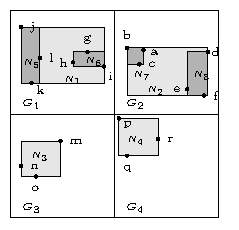
\includegraphics[width=\linewidth]{figs/knn/distributed-mrtree-data.pdf}
    \caption{Data}\label{fig:knn:distributed-mrtree:data}
  \end{subfigure}~%
  \begin{subfigure}[b]{.65\linewidth}
    \centering
    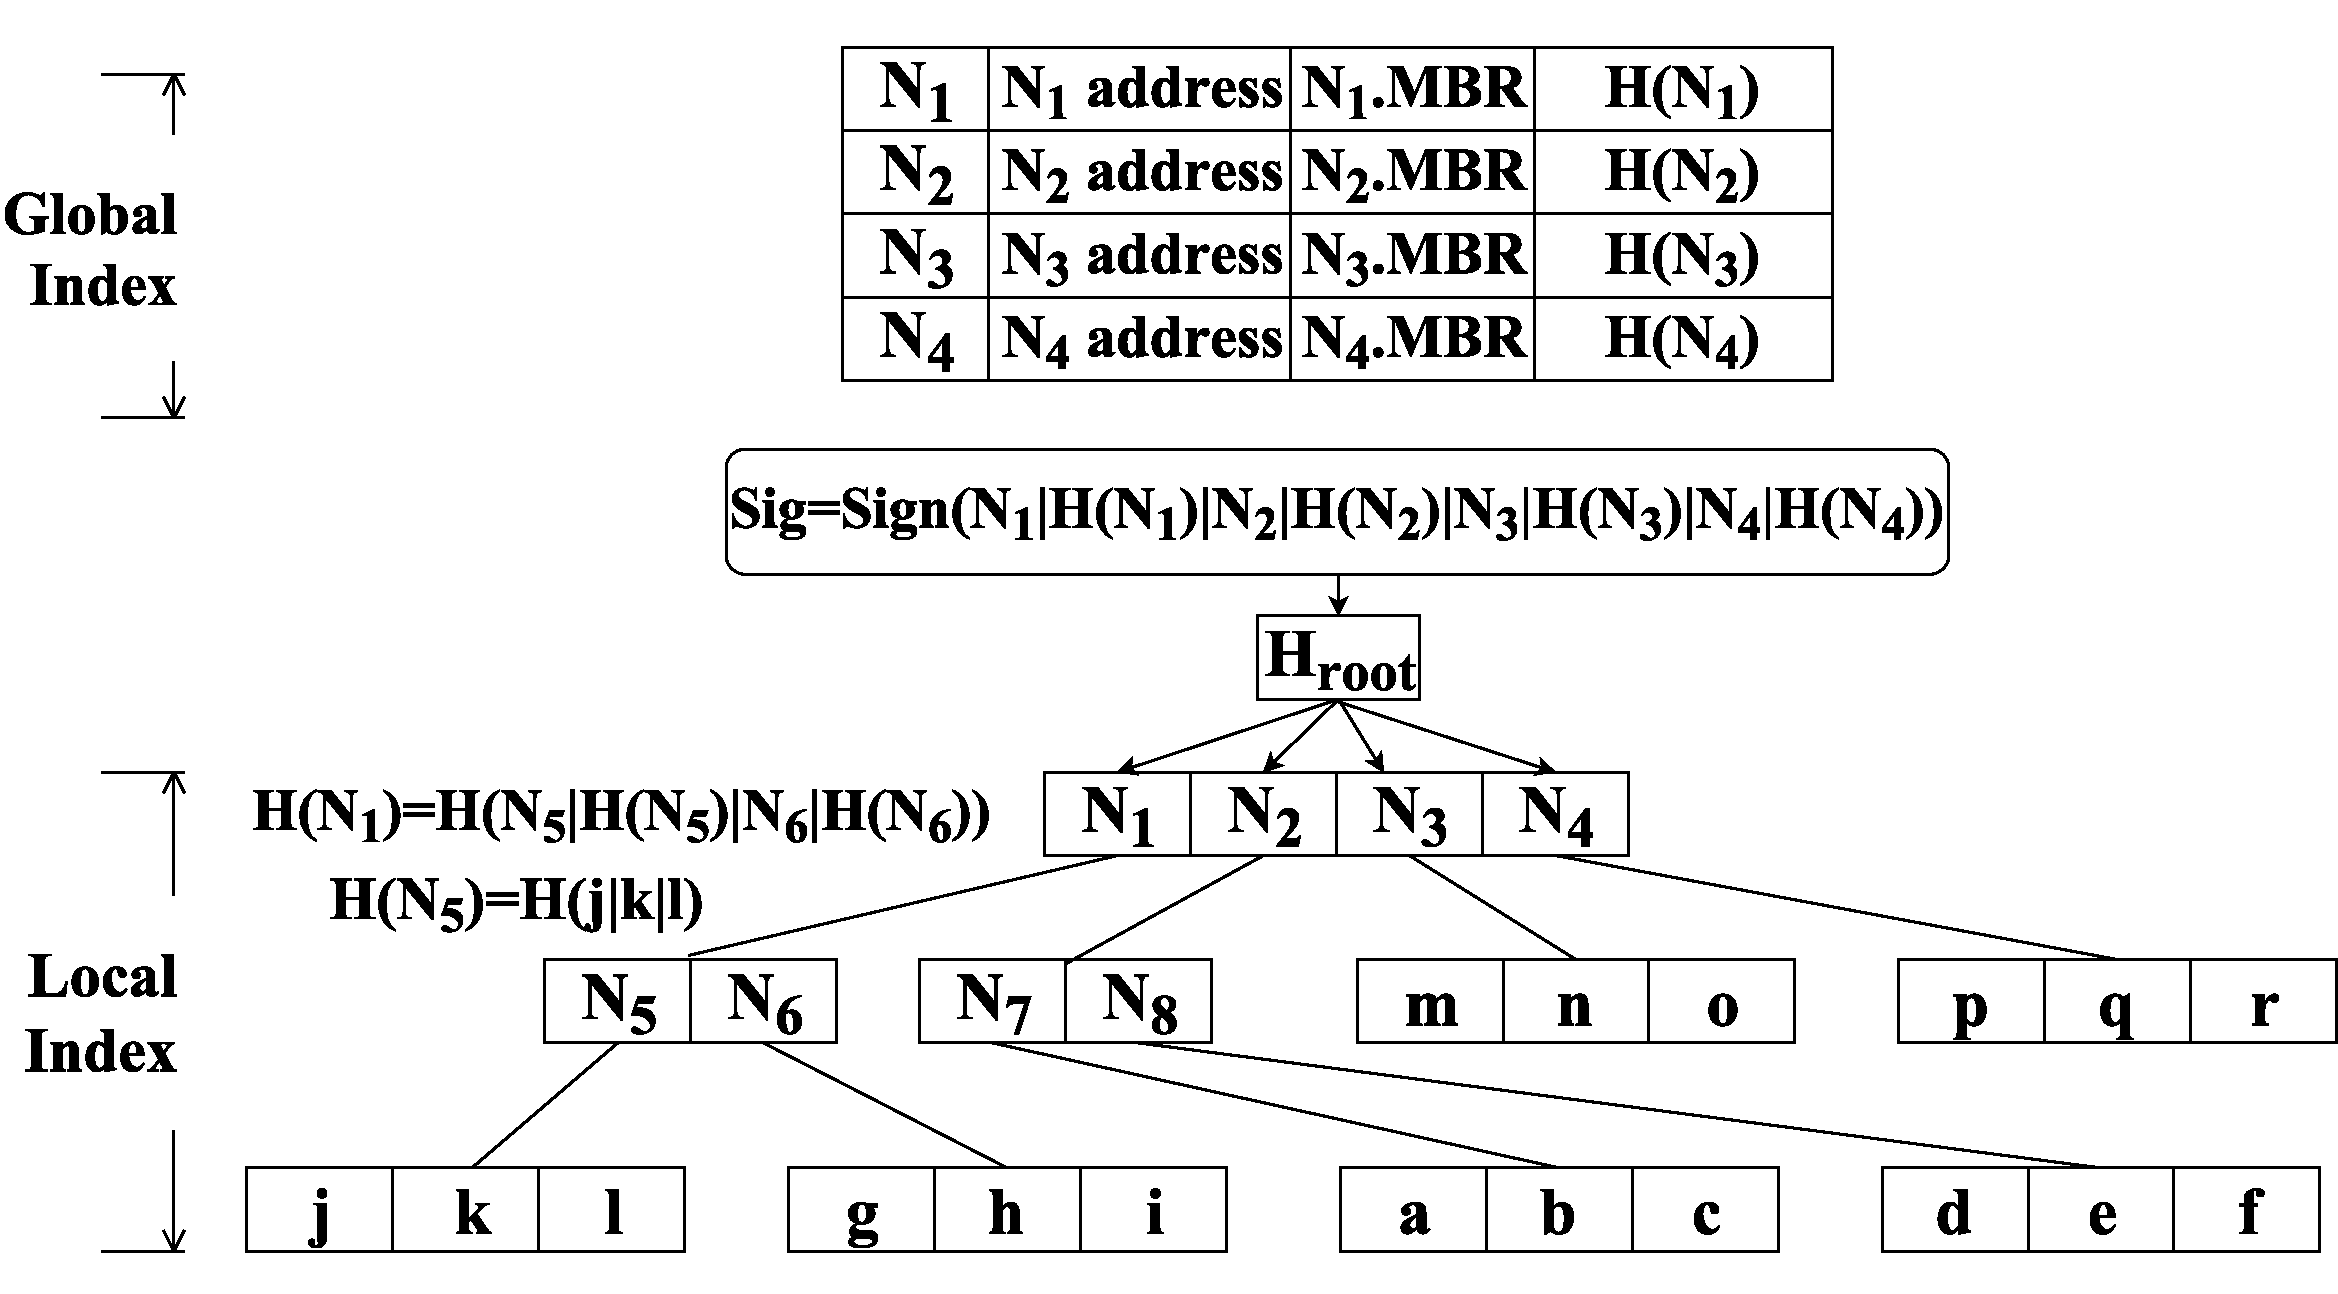
\includegraphics[width=\linewidth]{figs/knn/distributed-mrtree-tree.pdf}
    \caption{Index}\label{fig:knn:distributed-mrtree:tree}
  \end{subfigure}
  \caption{Distributed MR-tree}\label{fig:knn:distributed-mrtree}
\end{figure}

To adapt the MR-tree index structure to the distributed environment, the index structure has two layers: the local index and the global index. The DO first employs the Grid partition or the Sort-Tile-Recursive~\cite{10.1109/ICDE.1997.582015} method to partition the entire dataset into several splits. These methods guarantee that there is no overlap between any two partitions' \emph{minimum bounding rectangles} (MBRs). Thanks to this non-overlapping characteristic, only a few partitions are used to process the kNN query, which saves the computation resources. The local indexes are constructed using the data points in each partition. The global index is then constructed, and it contains each local MR-tree's root MBR and, root hash value, and the pointers towards each local index. After the construction of the index structure, the DO signs the root node of the global index using the private key. Then, the signature and the entire index will be sent to the SP\@. The $Master$ of the SP is responsible for dispatching the local indexes to the $Slaves$ according to the current workload of the distributed system. Since the global index is small, it will be stored in the main memory of all the nodes, which can speed up the kNN query processing. \Cref{fig:knn:distributed-mrtree:data} shows the four partitions using the Grid partition method. \Cref{fig:knn:distributed-mrtree:tree} depicts the entire structure of distributed MR-tree. In each partition, the data points are used to build a local MR-tree. We use $N_{1}$, $N_{2}$, $N_{3}$ and $N_{4}$ to represent the four local indexes. The global index is a directory table and can prune the search space.

\subsection{Authenticating Distributed kNN Query Processing}

For easy illustration, we first give some definitions, which will be used in the authenticating distributed kNN query processing.

\begin{definition}\label{def:knn:def1}
  Given a query point $q$ and a set of local MR-trees $T = \{T_{1}$, $T_{2}$, $\dots$, $T_{n}\}$, $T_{i}$ is a \emph{home index} if $dist(q,T_{i}.MBR) < dist(q,T_{j}.MBR)$ where $i, j\in [1 \dots n]$ and $j \neq i$. Here the $dist(\cdot,\cdot)$ denotes the minimum distance between a point and a rectangle.
\end{definition}

\begin{definition}\label{def:knn:def2}
  Given a query point $q$ and a set of current partial kNN results $\{r_{1}, r_{2}, \dots, r_{k}\}$, a \emph{rcircle} is a circle centered at $q$ with the radius of $dist(q,r_{k})$. Here the $dist(\cdot,\cdot)$ denotes the Euclidean distance.
\end{definition}

\begin{definition}\label{def:knn:def3}
  Given a \emph{rcircle} and a set of local MR-trees $T = \{T_{1}, T_{2}, \dots, T_{n}\}$, $CT$ is a set of \emph{candidate trees} if $CT \subseteq T$ and for each $CT_{i} \in CT$, $CT_{i}.MBR \cap \text{\emph{rcircle}} \neq \emptyset$ and $CT_{i} \neq \text{\emph{home index}}$.
\end{definition}

\begin{definition}\label{def:knn:def4}
  Given a set of slave nodes $Slaves = \{Slave_{1}, \dots, Slave_{n}\}$, a \emph{home slave} $HSlave \in Slaves$ is the slave which stores the \emph{home index}. And a set of \emph{candidate slaves} $CSlaves\subseteq Slaves$ are the set of slaves which stores \emph{candidate trees CT}.
\end{definition}

\begin{definition}\label{def:knn:def5}
  We define the VO computed by \emph{HSlave} is $hVO$; the VO computed by \emph{CSlaves} is $cVO$; the VO of non-processed slaves is $nVO$.
\end{definition}

\begin{definition}\label{def:knn:def6}
  We define the results computed by \emph{HSlave} are in \{$rs_{h}$\}; the results computed by \emph{CSlaves} are in \{$rs_{c}$\}.
\end{definition}

We assume that in the distributed system, queries are executed by the slaves who store the corresponding local indexes. For example, since the $HSlave$ stores the \emph{home index}, the first local kNN query should be sent to the $HSlave$ by the $Master$ and the $HSlave$ will execute the query locally.

\begin{figure}[t]
  \centering
  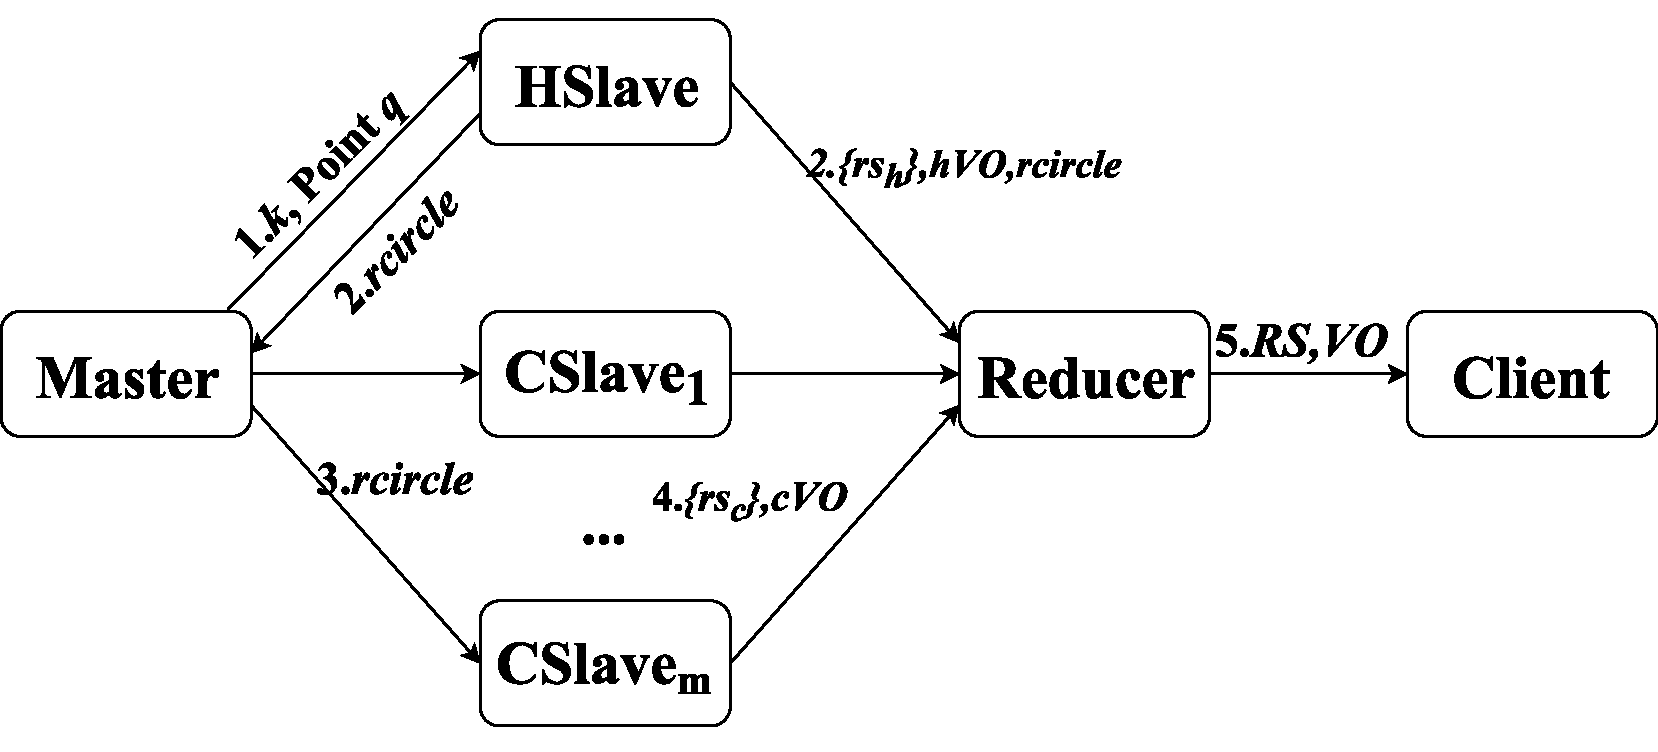
\includegraphics[width=.7\linewidth]{figs/knn/framework.pdf}
  \caption{Framework of Distributed Authenticated kNN Query}\label{fig:knn:frame}
\end{figure}

Our query authentication framework consists of three main procedures:
\begin{inlineenum}
\item the $HSlave$ processes the local authenticated kNN query to compute \{$rs_{h}$\} and $hVO$;
\item $CSlaves$ process additional range queries to compute \{$rs_{c}$\} and the $cVO$;
\item the $Reducer$ finally selects the $k$ nearest results from the partial results and generates the overall VO\@.
\end{inlineenum}
\Cref{fig:knn:frame} depicts the overview of the basic distributed kNN query processing.

The main objective is to use a small amount of partitions to compute the correct kNN results as well as the VO\@. The non-overlapping characteristic of the partition method prunes some local indexes, which saves the computation resources. The $HSlave$ first finds the local kNN results in the \emph{home index} which contains the correct results in a high probability. However, if there are some other points which are closer than the ones in $\{rs_{h}\}$, $CSlaves$ need to process extra range queries to find the correct results. The $rcircle$ is used to check whether $CSlaves$ should process the extra queries. \Cref{alg:knn:master} summarizes the procedure of the $Master$ node and the $Reducer$ node. The procedure of the $HSlave$ and the $CSlave$ is omitted because they simply compute the local queries and send the partial VO and results to the $Reducer$.

\begin{algorithm}[t]
  \caption{Distributed Authenticated kNN Procedure}\label{alg:knn:master}
  \SetKwBlock{MProc}{Master Procedure}{}
  \SetKwBlock{RProc}{Reducer Procedure}{}
  \MProc{%
    \KwIn{$k$, Point $q$}
    \KwOut{kNN request, range query requests}
    Send $kNN$ request to $HSlave$\;
    Receive $rcircle$, decide $CT$ list and $CSlaves$\;
    \If{$CT \neq \emptyset$}{
      Send \emph{range query} with $rcircle$ to the $CSlaves$\;
    }
  }
  \RProc{%
    \KwIn{$rs_{h}$, $hVO$, $rcircle$, $rs_{c}$, $cVO$}
    \KwOut{$RS$, $VO$}
    Receive $rs_{h}$, $hVO$, $rcircle$ from $HSlave$\;
    Compute $CT$ list using $rcircle$ and global index\;
    \eIf{$CT = \emptyset$}{%
      Add $hVO$ and $nVO$ to $VO$\;
      Send $rs_{h}$ and $VO$ to the $Client$\;
      }{%
      Receive \{$rs_{c}$\} and $cVO$ from $CSlaves$\;
      Add $k$ nearest results in $rs_{c}\cup rs_{h}$ to $RS$\;
      Add $hVO$, $cVO$, $nVO$ to $VO$\;
      Send $RS$ and $VO$ to the $Client$\;
    }
  }
\end{algorithm}

After receiving the kNN query from the client, the $Master$ locates the \emph{home index} and sends the kNN query request to the \emph{HSlave}. The $hVO$, $\{rs_{h}\}$ and $rcirlce$ will be computed by $HSlave$ using \Cref{alg:knn:knn} and are sent to the $Reducer$. Also, the $rcirlce$ is sent to the $Master$. Given the $rcircle$, the \emph{candidate trees} and the corresponding $CSlaves$ are identified (\Cref{def:knn:def3} and \Cref{def:knn:def4}) by the $Master$. When the $CT$ list is not empty, the $rcircle$ is sent to the $CSlaves$ by the $Master$. Each of the $CSlaves$ computes the local range query in parallel. The $Reducer$ consolidates $rs_{h}$, $\{rs_{c}\}$, $hVO$, $cVO$, and $nVO$. Then, it selects $k$ nearest results from the union of $\{rs_{h}\}$ and $\{rs_{c}\}$. The final VO list consists of $hVO$, $cVO$, and $nVO$. The $nVO$ can be derived using the global index and the $rcircle$. If a local index's MBR does not intersect with the $rcircle$, the MBR and hash value of the index will be added into $nVO$.

\begin{figure}[t]
  \centering
  \begin{subfigure}[b]{.33\linewidth}
    \centering
    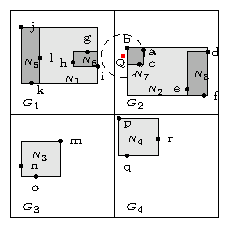
\includegraphics[width=\linewidth]{figs/knn/case1.pdf}
    \caption{Case 1}\label{fig:knn:cases:case1}
  \end{subfigure}~%
  \begin{subfigure}[b]{.33\linewidth}
    \centering
    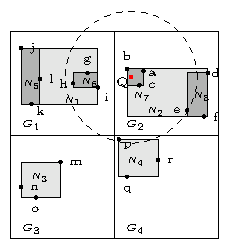
\includegraphics[width=\linewidth]{figs/knn/case2.pdf}
    \caption{Case 2}\label{fig:knn:cases:case2}
  \end{subfigure}~%
  \begin{subfigure}[b]{.313\linewidth}
    \centering
    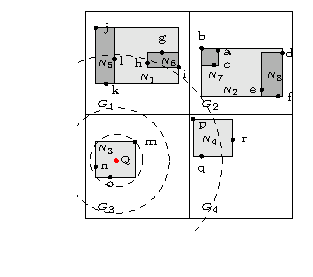
\includegraphics[width=\linewidth]{figs/knn/specialcase.pdf}
    \caption{Special Case}\label{fig:knn:cases:specialcase}
  \end{subfigure}
  \caption{Three Cases of {kNN} Processing}\label{fig:knn:cases}
\end{figure}

\Cref{fig:knn:cases} shows some cases of the distributed kNN processing. In case 1, we assume that $k$ equals $3$ and $Q$ is the query point. According to \Cref{def:knn:def1}, the \emph{home index} is $N_{2}$. Then the $Master$ sends the kNN request to the corresponding \emph{HSlave}. The $\{rs_{h}\}$ includes $\{b, c, a\}$ and the $hVO$ is $\{$[[$a, b, c$], [$N_{8}, H(N_{8})$]]$\}$. Since the $rcircle$ has no intersection with other local tree's MBR, the $CT$ list is empty. The non-processed VO set $nVO$ is \{[$N_{1}$, $H(N_{1})$], [$N_{3}$, $H(N_{3})$], [$N_{4}$, $H(N_{4})$]\}. Finally, the $Reducer$ sends the union of $hVO$ and $nVO$ and the results to the client.

In case 2, we assume that $k$ equals $4$. The query point $Q$ locates in $N_{2}$. The corresponding $HSlave$ computes the $rs_{h}=\{b, c, a, e\}$ and also the $hVO=\{$[[$a, b, c$], [$d, e, f$]]$\}$. The radius of $rcircle$ is the distance between $Q$ and point $e$. Using the global index and $rcircle$, the $Master$ node finds the $CT=\{N_{1}, N_{4}\}$ and sends the range query requests to the $CSlaves$. The two local result sets ${\{rs_{c}\}}_{N_{1}}=\{g, h, i\}$ and ${\{rs_{c}\}}_{N_{4}}=\{p\}$ are computed by each $CSlave$. Meanwhile, $cVO=\{$[[$N_{5}, H(N_{5})$], [$g, h, i$]], [$p, q, r$]$\}$ is computed. The $Reducer$ selects the $4$ nearest result points from the union of partial results and the final result set is $RS=\{b, c, a, i\}$. The local tree $N_{3}$ does not intersect with the $rcircle$, so that [$N_{3}, H(N_{3})$] will be added to the $nVO$. The final VO consists of $hVO$, $cVO$, and $nVO$.

There is a special case of the distributed kNN processing when the number of data points in a partition is less than $k$. A skewed distribution of data points may lead to this case. The previous algorithm cannot compute the correct kNN results. In this case, we double the radius of the $rcircle$ and process the range query iteratively. The $Reducer$ checks the result number and sends the message to the $Master$ if the result number is less than $k$. The $Master$ doubles the $rcircle$'s radius and the new $rcircle$ is sent to the updated $CSlaves$. This process runs iteratively until the result number exceeds $k$. \Cref{fig:knn:cases:specialcase} illustrates the special case. Assume that $k$ is $4$ and $Q$ is the query point. $N_{3}$ is the \emph{home index}. During the third iteration, we find $8$ points and the iteration terminates. Finally, the $Reducer$ selects $4$ nearest points and returns the final $RS$ and $VO$ to the client. In this special case, the VO size is rather large since the radius of $rcircle$ grows exponentially. To avoid this case, in our experiments we use the Sort-Tile-Recursive (STR)~\cite{10.1109/ICDE.1997.582015} partition method to split the dataset. The STR partition splits the near data points in the same partition and each partition has nearly the same number of data points.

\subsection{Client Verification}\label{sec:knn:client-verification}

\begin{algorithm}[t]
  \caption{Client Verification}\label{alg:knn:client-verification}
  \KwIn{$k$, Point $q$, result set $RS$, verification object $VO$}
  \KwOut{Whether the result passes the verification}
  Receive ${root}_{DO}$ and check its signature with respect to DO's public key\;
  Reconstruct MB-tree ${root}$ using $VO$\;
  \lIf{${root}_{DO} \neq {root}$}{\Return{False}}
  Extract data points and MBRs from $VO$ and put them into $rs$, $mbr$ list\;
  Sort $rs$ by distance to $q$\;
  \For{$i=[1:k]$}{%
    \lIf{$RS[i] \neq rs[i]$}{\Return{False}}
  }
  \For{$obj$~\textnormal{\textbf{in}}~$mbr$}{%
    \lIf{$dist(q,RS[k])>dist(q,obj)$}{\Return{False}}
  }
  \Return{True}\;
\end{algorithm}

The client uses the VO to verify the results' soundness and completeness. The soundness is verified first by reconstructing the root hash value of the distributed MR-tree. The root hash value is the hash value of the concatenation of each local tree's MBR and hash value. If the reconstructed hash value matches the root hash signed by the public key of the DO, the soundness is satisfied. The completeness can be verified in the following method. All of the data points and MBRs are extracted from the VO set and the client selects the first $k$ nearest data points and compares them with the $RS$. If they match, it means that no other points are closer than the RS data points. Also, all of the $MBRs$ must be farther than the $k^{th}$ result point. \Cref{alg:knn:client-verification} summarizes the procedure of client's verification.

Take \Cref{fig:knn:cases:case2} as an example. The overall VO consists of $hVO=\{$[[$a, b, c$], [$d, e, f$]]$\}$, $cVO=\{$[[$N_{5}, H(N_{5})$], [$g, h, i$]], [$p, q, r$]$\}$ and $nVO=\{$[$N_{3}, H(N_{3})$]$\}$. The client can recompute $N_{2}$ using $hVO$. $N_{7}$, $N_{8}$ as well as their corresponding hash values are derived by $\{a, b, c\}$ and $\{d, e, f\}$, respectively. $H(N_{7})$ is the hash value of the concatenation of points $a$, $b$, and $c$. Similarly, $H(N_{8})$ can be computed. $N_{2}$ and $H(N_{2})$ are generated by $N_{7}$, $N_{8}$, and their hash values. Points $g$, $h$, and $i$ are used to compute $N_{6}$ and $H(N_{6})$. $N_{1}$ with its hash value can be derived by $N_{5}$, $N_{6}$, and their hash values. $N_{4}$ and $H(N_{4})$ are computed using points $p$, $q$, and $r$ in $cVO$. The $N_{3}$ and $H(N_{3})$ are given in $nVO$. Therefore, the root hash value is computed using four local MR-trees' root hash values and MBRs. After that, the data points and MBRs are extracted from the union of VO\@. The correct results are $\{b, c, a, i\}$ and all of the non-result points will be checked whether they are closer than point $i$. Meanwhile, the MBR of $N_{5}$ and $N_{3}$ are checked whether they are farther from point $i$.

\subsection{Robustness Analysis}

\begin{lemma}\label{lem:knn:l1}
  If there is no need to invoke the range queries ($CT=\emptyset$), the local kNN result $rs_{h}$ will be the final correct results.
\end{lemma}

\begin{proof}
  This can be proved by contradiction. If there is a point $p$ which is one of the correct kNN results but not included in the local kNN result, it is either inside or outside the partition. If it is inside the partition, it should be outside the $rcircle$ since all of the points in the $rcirlce$ are added into $rs_{h}$. There are $k$ points inside the $rcircle$, so $p$ must be at least ${(k+1)}^{th}$ nearest point. This contradicts the assumption that it is one of the correct results. If it is outside the partition, as there is no intersection among the partitions, it must be farther than the current $k^{th}$ result and this contradicts the correct result assumption.
\end{proof}

\begin{lemma}\label{lem:knn:l2}
  All of the correct kNN results must reside in the $rcircle$.
\end{lemma}

\begin{proof}
  This can be proved by contradiction. Suppose there is a correct kNN result $p$ which resides outside the $rcircle$. The radius of $rcircle$ is computed by the distance between the $k^{th}$ current nearest point and the query point. There are at least $k$ data points inside the $rcircle$ because apart from the $k$ local results, there are probably some points in other partitions that are closer than the current $k^{th}$ point. Since $p$ is outside the $rcircle$, it is at least the ${(k+1)}^{th}$ nearest point, which contradicts the assumption.
\end{proof}

\begin{theorem}
  \Cref{alg:knn:master} can produce the correct result set.
\end{theorem}

\begin{proof}
  This can be proved using \Cref{lem:knn:l1} and \Cref{lem:knn:l2}.
\end{proof}

\Cref{alg:knn:client-verification} summarizes the procedure of client verification. The root hash reconstruction guarantees the \emph{soundness} of the results and the distance comparison protects the \emph{completeness}. We now give the following theorem of its correctness of verification.

\begin{theorem}\label{thm:knn:verify}
  \Cref{alg:knn:client-verification} verifies the soundness and completeness of the results and can detect the threats mentioned in \Cref{sec:knn:problem}.
\end{theorem}

\begin{proof}
  If the adversary returns a fictitious point, which is not included in the dataset, the reconstructed root hash must be different from the signed hash value received from the DO because of the collision-resistance characteristic of the hash function. If one data point changes, its corresponding hash value will be different, resulting in the change of the root hash value of MR-tree. Without knowing the secret key, the SP cannot generate a valid signature of the wrong root hash value, which means that the signature is unforgeable. Therefore, the violation of soundness can be detected. If the reconstructed hash value matches the signed one, the incorrect result point must reside in the VO set but farther than the correct results. After the client sorts all the data points in the VO set by distance and gets the first $k$ nearest points, the client can notice the difference between $k$ points extracted from the VO and the points in RS\@. Then the results cannot pass the verification of the completeness.
\end{proof}

\section{Optimization of VO size}\label{sec:knn:opt}

The VO size determines the communication cost and also the client verification time. In this section, we focus on the optimization of the VO size. Intuitively, the $rcircle$ decides the VO size. A larger $rcircle$ makes more nodes to be visited and hence and more data points to be added to the VO\@. Therefore, the objective is to reduce the radius of the $rcircle$. As we can see in \Cref{fig:knn:cases:case2}, the $rcircle$ is much bigger than the circle with the radius of the distance between $Q$ and point $i$. This is because the distance between $Q$ and $e$ is larger than the distance between $Q$ and $i$. In \Cref{alg:knn:master}, the $rcircle$ is decided by the local results in \emph{home index} and will not change during the whole procedure. To compute the minimum $rcircle$, the optimized algorithm adds the sequential computation of the $rcircle$ before the parallel authenticated range query in \Cref{alg:knn:master}.

\begin{algorithm}[t]
  \caption{VO Optimization Algorithm}\label{alg:knn:opt}
  \SetKwBlock{MProc}{Master Procedure}{}
  \MProc{%
    \KwIn{$k$, Point $q$}
    \KwOut{kNN request, range query requests}
    Send $kNN$ request to $HSlave$\;
    Receive $rcircle$\;
    Compute $CT$ list and decide $CSlaves$\;
    \If{$CT \neq \emptyset$}{%
      Sort $CT$ list with minimum distance\;
      \For{$i = [1:|CT|]$}{%
        \lIf{$rcircle$ not intersects $CT[i].MBR$}{\textbf{break}}
        Send $rcircle$ to $CSlave[i]$\;
        Receive $rs_{c}$\;
        $rs_{h} \gets rs_{h} + rs_{c}$\;
        Select $k^{th}$ nearest point $obj$ in $rs_{h}$\;
        Update $rcircle$'s radius with $dist(obj, q)$\;
      }
      Recompute $CSlaves$ using final $rcircle_{f}$\;
      Send $rcircle_{f}$ to $HSlave$ and $CSlaves$\;
    }
  }
\end{algorithm}

\Cref{alg:knn:opt} summarizes the procedure of the $Master$ node. The procedure of slaves is omitted because they simply compute the partial results and VOs. First, the $Master$ sends the kNN request to the $HSlave$ and uses the received $rcircle$ to decide the candidate tree list $CT$ and $CSlaves$. If the $CT$ list is not empty, the $Master$ sequentially updates the $rcircle$. Since the closer local indexes have the kNN results in a higher probability, the $CT$ list is sorted with the minimum distance. In the \emph{for} loop in \Cref{alg:knn:opt}, the $rcircle$ will be sequentially sent to each $CSlave$ and the $rs_{c}$ will be added into $rs_{h}$ to find the current $k^{th}$ nearest point $obj$, which is used to update the $rcircle$. Note that the \emph{for} loop terminates immediately when the updated $rcircle$ does not intersect with the $CT[i].MBR$. This prunes some search space and improves the performance. The $CSlaves$ list is recomputed after the computation of the final $rcircle$. Since the $rcircle$ changes, the $rs_{h}$ and $hVO$ are recomputed. Also, the $Reducer$ should discard the previously received $rs_{h}$ and $hVO$ when it finds that $CT$ list is not empty. The $Master$ sends the $rcircle_{f}$ to the $HSlave$ and the $CSlaves$, which compute the range query and VOs in parallel. The $Reducer$ receives all kinds of results and $VOs$ from the $Slaves$. Then it selects $k$ nearest results and adds them to the $RS$ list. The $nVO$ is also added into the $VO$. Finally, the $RS$ and $VO$ are sent to the $Client$.

\begin{figure}[t]
  \centering
  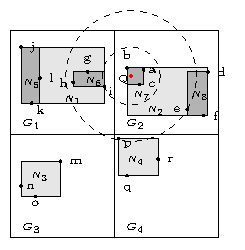
\includegraphics[width=.4\linewidth]{figs/knn/optimize.pdf}
  \caption{Example of optimization of VO size}\label{fig:knn:opt}
\end{figure}

\Cref{fig:knn:opt} shows an example of the VO optimization. We assume that $k=4$ and the query point $Q$ lies in $N_{2}$. The \emph{home index} is $N_{2}$ and the ordered $CT$ list is $\{N_{1}, N_{4}\}$. The outer dashed circle is the initial $rcircle$ computed using the $\{rs_{h}\}$. The $hVO$ is $\{$[[$a, b, c$], [$d, e, f$]]$\}$. Then the range query will be processed on $N_{1}$ first. The result of the range query $rs_{c}$ is $\{g, h, i\}$. The $Master$ next finds the point $i$, which is the $4^{th}$ result in the union of $\{rs_{c}\}$ and $\{rs_{h}\}$. The $rcircle$ will be updated to the smaller dashed circle in \Cref{fig:knn:opt}. Since the updated $rcircle$ does not intersect with the next local index $N_{4}$ in the $CT$ list, the \emph{for} loop terminates. The $CT$ list and the $CSlaves$ are recomputed. The $rcircle_{f}$ will be sent to the $HSlave$ and $CSlave$ storing $N_{2}$ and $N_{1}$, respectively. The $Reducer$ receives $rs_{h} = \{a, b, c\}$, $hVO= $[[$a, b, c$], [$N_{8}, H(N_{8})$]], $rs_{c} = \{i\}$, and $cVO =$[[$N_{5}, H(N_{5})$], [$g, h, i$]]. The final results contain $\{b, c, a, i\}$. The $nVO$ contains [$N_{3}, H(N_{3})$] and [$N_{4}, H(N_{4})$]. The updated $rcircle$ avoids the visit of local index $N_{4}$ and also the subtree $N_{8}$. Therefore the VO size is reduced by this algorithm.

In \Cref{alg:knn:opt}, the $rcircle$ is updated iteratively in the \emph{for} loop. The definition of the $rcircle$ remains to be the same. As such, the correctness of results and VO generation can still be proved using \Cref{lem:knn:l1} and \Cref{lem:knn:l2}.

Obviously, \Cref{alg:knn:opt} spends more time than \Cref{alg:knn:master} in query processing because of the sequential update of $rcircle$. If the $|CT|$ is large, the sequential update consumes too much time. Therefore, we design a hybrid algorithm, in which the $rcircle$ is updated only for $l$ times, where $1\le l \le |CT|$. Here the value $l$ denotes the level of sequential processing. After $l$ sequential queries, we resort to \Cref{alg:knn:master} for parallel processing of distributed authentication. The hybrid algorithm uses less range queries to find the optimized $rcircle$ and it balances the trade-off between the VO size and the query time. Note that if the $|CT|$ equals one, the hybrid algorithm and the optimized algorithm are the same because there is only one update of the $rcircle$.

%
\chapter{Conclusions}\label{chap:conclusions}

In this dissertation, we have tackled three kinds of query authentication problems, namely authentication of aggregate queries over set-valued data, authentication of relational queries with fine-grained access control, and authentication of {kNN} queries in distributed environment. They enables the DO outsourcing the data and query services to an untrusted third party cloud while still maintaining data integrity. Furthermore, they addresses a variety of needs demanded by enterprise customs such as supporting aggregate queries over set-valued data, enforcing fine-grained access control, and conforming distributed environment. Security analysis and performance evaluation show that the proposed solutions and techniques are robust and efficient under a wide range of system settings.

\section{Contributions}

The first contribution of this dissertation is the development of the query authentication algorithms that support aggregate queries over set-valued data. To the best of our knowledge, this is the first work that addresses both integrity and confidentiality for aggregate queries over set-valued data. We propose a privacy-preserving authentication framework and we develop a set of privacy-preserving authentication protocols and algorithms for various aggregate queries. Formal security analysis and cost models for the proposed authentication protocols and algorithms are also given. To further enhance the performance of query authentication algorithms, we propose several optimizations. Finally, we perform extensive performance evaluation on real-world datasets. Empirical results demonstrate the feasibility and robustness of our proposals.

The second contribution of this dissertation is the study of combining query authentication and access control. To the best of our knowledge, this is the first work on query authentication for databases with fine-grained access control. We believe that this is a timely study, as enterprise cloud database systems dictate integrity (query authentication) and authorization (access control) at the same time. We propose a novel ABS-based APP signature as the primitive for ADS, together with a grid-index-based tree structure that can aggregate APP signatures for efficient range and join query authentication. To further improve the query performance, we develop several optimization techniques that are either compatible with the original security model or a relaxed one. Furthermore, we conduct a security analysis and empirical study on the authentication performance with respect to various factors such as query range size and database cardinality.

The third contribution of this dissertation is an investigate authenticated kNN query processing in a distributed environment.We propose distributed MR-tree as an ADS to suit the distributed query processing environment. We develop a basic algorithm and two optimization techniques to efficiently process authenticated kNN queries in a distributed fashion. We also conduct extensive experiments to validate the performance of the proposed techniques in terms of query cost, communication overhead, and verification time.

\section{Possible of Future Work}

As for future work, we plan to extend the proposed privacy-preserving authentication techniques developed in \Cref{chap:aggregate-queries} to more complex aggregate queries such as median and percentile. We also plan to leverage GPGPU technologies to accelerate the computation of accumulative values during query processing at the SP\@.

For the study of enforcing access control, we plan to extend the proposed techniques in \Cref{chap:access-control} to support more complex queries, such as aggregation. We also plan to study more challenging fine-grained query authentication problems for multi-source data in a distributed environment.

Finally, we plan to design a distributed spatial query authentication system to support more spatial queries and efficient data updates based on what we learn in \Cref{chap:knn}.
%
\appendix%
\chapter{Proof of \texorpdfstring{\cref*{thm:aggregate-queries:sec}}{Theorem~\ref{thm:aggregate-queries:sec}}}%
\label{app:aggregate-queries}

We start by proving the security of the privacy-preserving authentication protocols on multiset operations. Note that the proofs of $sub(\cdot, \cdot)$ and $empty(\cdot)$ are similar to those on set operations in~\cite{10.1007/978-3-642-22792-9_6} and are hence omitted.

\section{Security of $sum(\cdot)$ Operation}

\begin{lemma}[Security of $sum(\cdot)$ operation]\label{lem:aggregate-queries:sum}
  Under the bilinear $q$-strong Diffie-Hellman assumption, if the accumulative value returned by $sum(\{X_1,\dots,X_n\})$ passes the client's verification, then the probability of $sum(\{X_1,\dots,X_n\}) \neq acc(\uplus_{i=1}^n X_i)$ is negligible for any PPT adversary.
\end{lemma}

\begin{proof}
  First, we prove that this lemma holds for $n=2$ by contradiction. Support there is a PPT algorithm that computs such a multiset $S = \{y_1, \dots, y_{\ell}\}$, whereas $y_j \notin X_1 \uplus X_2$ for some $1 \le j \le \ell$. This means that
  \begin{align*}
    e(acc(X_1), acc(X_2)) &= e(g^{\prod_{y \in S} (y+s)}, g) \Rightarrow \\
    {e(g, g)}^{\prod_{x \in X_1 \uplus X_2} (x+s) } &= {e(g, g)}^{\prod_{y \in S} (y+s)}
  \end{align*}
  Note that $(y_j + s)  \nmid \prod_{x \in X_1 \uplus X_2} (x+s)$. Therefore, there exists a polynomial $Q(s)$ (computable in polynomial time) of degree $n-1$ and constant $\lambda \neq 0$, such that $\prod_{x \in X_1 \uplus X_2} (x+s) = Q(s)(y_j + s) + \lambda$. Thus, we have
  \begin{align*}
& {e(g, g)}^{(y_j + s)\prod_{1 \le i \neq j \le \ell} (y_i+s)} = {e(g,g)}^{Q(s)(y_j + s) + \lambda} \Rightarrow \\
& {e(g, g)}^{1/(y_j + s)} = {\left[ {e(g,g)}^{\prod_{1 \le i \neq j \le \ell} (y_i+s)} {e(g,g)}^{-Q(s)} \right]}^{\lambda^{-1}}.
  \end{align*}
  Thus, this algorithm can break the bilinear $q$-strong Diffie-Hellman assumption. This proves that our lemma holds for $n=2$.

  Supposing our lemma is true for any $n=k$, where $k\ge 2$, in the following we prove it is also true for $n=k+1$. Let $\varepsilon_k$ denote the event that \textsf{Adv} returns incorrect accumulative value $sum(\uplus_{i=1}^{k} X_i)$ and passes the client's verification. By law of probability, we have:
  \begin{align*}
    \Pr[\varepsilon_{k+1}] &=  \Pr[\varepsilon_{k}]\Pr[\varepsilon_{k+1} | \varepsilon_{k}] +
    \Pr[\varepsilon_{k}']\Pr[\varepsilon_{k+1} | \varepsilon_{k}']\\
                           &\leq \Pr[\varepsilon_{k}] + \Pr[\varepsilon_{k+1}|\varepsilon_{k}'] \\
                           &= \Pr[\varepsilon_{k}] + \Pr[\varepsilon_{2}],
  \end{align*}
  where $\varepsilon'$ denotes the complement of an event. Finally, we have:
  \begin{align*}
    \Pr[\varepsilon_n] \leq (n-1) \Pr[\varepsilon_2]
  \end{align*}
  Since $\Pr[\varepsilon_2]$ is negligible according to our proof for $n=2$, we can conclude that $\Pr[\varepsilon_{n}]$ is negligible as $p\gg n$ in a cyclic multiplicative group $\mathbb{G}$. Hence, this lemma is proved.
\end{proof}

\section{Security of $union(\cdot)$ Operation}

\begin{lemma}[Security of $union(\cdot)$ operation]\label{lem:aggregate-queries:union}
  Under the bilinear $q$-strong Diffie-Hellman assumption, if the accumulative value returned by $union(\{X_1,\dots,X_n\})$ passes the client's verification, then the probability of $union(\{X_1,\dots,X_n\}) \neq acc(\cup_{i=1}^n X_i)$ is negligible for any PPT adversary.
\end{lemma}
\begin{proof}
  Let $U = \cup_{i=1}^n X_i$. The $union(\cdot)$ protocol consists of three modules
  \begin{inlineenum}
  \item $sub(\widehat{X}_1, U)$, $sub(\widehat{X}_2, U)$, $\dots$, $sub(\widehat{X}_n, U)$;%
    \label{enum:aggregate-queries:union-proof:mod1}
  \item $empty(\{U-\widehat{X}_1, U-\widehat{X}_2, \dots, U -\widehat{X}_n\})$; and%
    \label{enum:aggregate-queries:union-proof:mod2}
  \item SP sends the ECRH hash value ${h_e(U)}^*$ for $U$.%
    \label{enum:aggregate-queries:union-proof:mod3}
  \end{inlineenum}
  Due to the composition property and the security of~\ref{enum:aggregate-queries:union-proof:mod1} and~\ref{enum:aggregate-queries:union-proof:mod2}, we only need to prove the security of~\ref{enum:aggregate-queries:union-proof:mod3}, that is, ${acc(U)}^*$ cannot be forged if ${h_e(U)}^*$ passes the client's verification. Denote $acc^{-1}({acc(U)}^*)$ as the set who has accumulator value ${acc(U)}^*$.

  First, we prove $acc^{-1}({acc(U)}^*)\subseteq U$, i.e., the returned value ${acc(U)}^*=g^{{P(U)}^*}$=$g^{P(U) \cdot Q_U(s)}$, where $Q_U(s)$ is some polynomial. We prove this by contradiction.
  We assume there exists an element $x_j \in \widehat{X}_i$ such that $(x_j + s) \nmid {P(U)}^*$, i.e., ${P(U)}^* = (x_i + s) \cdot Q_i(s) + \lambda_i$, where $Q_i(s)$ is some polynomial and $\lambda_i$ is a constant value. During the execution of protocol $sub(\widehat{X}_i, U)$, by expanding $e(acc(\widehat{X}_i), W_i^*) = e({acc(U)}^*, g)$, the adversary can get:
  \begin{align*}
    e(g^{\prod_{k=1}^{|\widehat{X}_i|}(x_k+s) }, W_i^*)  = {e(g, g)}^{(x_j+s) \cdot Q_i(s) + \lambda_i}.
  \end{align*}
  By dividing $(x_j+s)$ on the exponents of both sides, the adversary can get:
  \begin{align*}
    {e(g, W_i^*)}^{\prod_{k=1}^{j-1}{(x_k+s)} \cdot \prod_{k=j+1}^{|\widehat{X}_i|}{(x_k+s)}} = {e (g, g)}^{Q_i(s) + \lambda_i/(x_j+s)}.
  \end{align*}
  Finally, the adversary can get:
  \begin{align}
&{e(g, g)}^{1/(x_j + s)}  \nonumber \\
    = &{({e(g, W_i^*)}^{\prod_{k=1}^{j-1}(x_k+s) \cdot \prod_{k=j+1}^{|\widehat{X}_i|}{(x_k+s)}} \cdot {e(g, g)}^{-Q_i(s)})}^{1/\lambda_i},\nonumber
  \end{align}
  which violates the bilinear $q$-strong Diffie-Hellman assumption mention in \cref{sec:aggregate-queries:prelim}. Hence, by contradiction, ${P(U)}^*$ must be in the form of $P(U) \cdot Q_U(s)$.

  Next, we prove $U \subseteq acc^{-1}({acc(U)}^*)$, i.e., $Q_U(s)$ can only be a constant value. We prove this by contradiction. For each set $\widehat{X}_i$, ${acc(U - \widehat{X}_i)}^* = g^{P(U-\widehat{X}_i) \cdot Q_U(s)}$. During the execution of $empty(\cdot)$, by expanding $\prod_{i=1}^n e({acc(U-\widehat{X}_i)}^*, F_i^*)=e(g, g)$, the adversary can get:
  \begin{align*}
    \prod_{i=1}^n e(g^{P(U-\widehat{X}_i)}, g^{Q_i(s)}) = e(g, g),
  \end{align*}
  and then
  \begin{align*}
    {e(g,g)}^{Q_U(s)(\prod_{i=1}^n P(U-\widehat{X}_i)\cdot Q_i(s))}=e(g,g).
  \end{align*}
  Finally, the adversary can get:
  \begin{align*}
    {e(g, g)}^{1/Q_U(s)} = {e(g, g)}^{P(U-\widehat{X}_i \cdot Q_i(s))}.
  \end{align*}
  Since $Q_U(s)$ is a polynomial whose order is larger than $1$, the adversary violates the bilinear $q$-strong Diffie-Hellman assumption. Thus, by contradiction, $Q_U(s)$ must be a constant value.

  By the above two arguments, we prove that the accumulative value ${acc(U)}^*$ cannot be forged if it passes the client's verification.
\end{proof}

\section{Security of $times(\cdot, \cdot)$ Operation}

\begin{lemma}[Security of $times(\cdot,\cdot)$ operation]\label{lem:aggregate-queries:times}
  Under the bilinear $q$-strong Diffie-Hellman assumption, if the accumulative value returned by $times(X,t)$ passes the client's verification, then the probability of $times(X,t) \neq acc(\uplus_{i=1}^t X)$ is negligible for any PPT adversary.
\end{lemma}
\begin{proof}
  The $times(\cdot, \cdot)$ operation relies only on the $sum(\cdot)$ operation, and therefore the proof is similar to that of \cref{lem:aggregate-queries:sum}.
\end{proof}

\section{Security of PA$^2$ Algorithms}

Following the above lemmas, we now show that the query results returned by the PA$^2$ algorithms cannot be forged.
\aggregatesecuritytheorem*

\begin{proof}
  According to the lemmas on the security of operations $sub(\cdot,\cdot)$, $empty(\cdot)$, $sum(\cdot)$, $union(\cdot)$, $times(\cdot,\cdot)$, the theorem is trivially true due to the composition property.
\end{proof}

%
\chapter{Proof of \texorpdfstring{\Cref*{thm:access-control:abs-sec}}{Theorem~\ref{thm:access-control:abs-sec}}}%
\label{app:access-control-abs-sec}

\abssecuritytheorem*

The theorem is proved by showing our ABS scheme satisfies each security property.

\section{Proof of Perfect Privacy}

\begin{lemma}\label{lemma:access-control:abs-privacy}
  Our scheme has perfect privacy according to \Cref{def:access-control:abs-privacy}.
\end{lemma}

\begin{proof}
  The first requirement of \Cref{def:access-control:abs-privacy} is trivial considering the scheme is derived from~\cite{10.1007/978-3-642-19074-2_24}. It is also easy to verify that the distributions of the output signatures from \textsf{ABS.Sign} and \textsf{ABS.Relax} are identical owing to the re-randomization step in \textsf{ABS.Relax}, which proves the second requirement.
\end{proof}

\section{Proof of Unforgeability}

\begin{lemma}\label{lemma:access-control:abs-unf}
  Our scheme is unforgeable according to \Cref{def:access-control:abs-unf} in the generic group model.
\end{lemma}

\newcommand{\Lin}{\textsf{Lin}}
\newcommand{\Hom}{\textsf{Hom}}

\begin{proof}
  The generic group model is designed to model the behavior of any algorithm that does not exploit the algebraic structure of the underlying groups. In other words, the lemma guarantees that our proposed scheme is unforgeable against any generic attacker, i.e., the attacker that does not exploit the underlying group structures. We remark that the scheme in~\cite{10.1007/978-3-642-19074-2_24} is also analyzed in this setting.

  The idea of the generic group model is briefly reviewed here. Let $p$ be a prime which represents the group order. A generic group $\mathbb{G}_i$ can be represented as the set $\{\xi_i(x)| x\in\mathbb{Z}_p\}$. The group operations are modeled by two oracles, namely, $\mathcal{O}_1, \mathcal{O}_2$. Specifically, on input two group elements $\xi_i(a), \xi_i(b)$, oracle $\mathcal{O}_i$ returns $\xi_i(a+b)$ and $\xi_i(a-b)$ respectively for multiplication and division. To model the bilinear pairing, another oracle $\mathcal{O}_E$ is defined. On input elements $\xi_1(a)$, $\xi_1(b)$, $\mathcal{O}_E$ returns $\xi_2(ab)$. Given $\xi_i(x)$ and scalar $s$, it is possible to obtain $\xi_i(sx)$ (via $O(\log s)$ calls to oracle $\mathcal{O}_i$).

  Since it only benefits the attacker, we assume the groups $\mathbb{G}$ and $\mathbb{H}$ are the same. The groups $\mathbb{G}$, $\mathbb{G}_T$ of the scheme are modeled as generic groups $\mathbb{G}_1$ and $\mathbb{G}_2$, respectively. The attacker works with the group elements and can only compute group operations by interacting with oracles $\mathcal{O}_i$ and $\mathcal{O}_E$. As the encoding functions $\xi_i$ are modeled as random functions, nothing about the element except equality can be inferred. The security proof is completed by showing that given the encodings of the public key and the signatures from the signing oracle, it is infeasible to output the encodings needed to satisfy the verification equation for the forgery with a bounded number of queries to oracles $\mathcal{O}_i$ and $\mathcal{O}_E$.

  We first define how signature queries are answered. For span program $\mathbf{M}\in \mathbb{Z}_p^{\ell \times t}$ with row labeling function $u$, pick random $\tau, y, s_1, \dots, s_\ell$, compute $p_j$ for $j=1$ to $t$, as follows:
  \begin{align*}
    p_j = \frac{1}{c + \hash}\big(\sum_{i=1}^\ell s_i (a+u(i)b)\mathbf{M}_{ij} - yz_j\big),
  \end{align*}
  where $(z_1, \dots, z_\ell) = (1, 0, \dots, 0)$ and $\hash = H(\tau$, $m)$.

  The signature is parsed as $\sigma=(\tau, g^y, g^{y/a_0}, g^{s_1}, \dots, g^{s_\ell}, h^{p_1}, \dots, h^{p_t})$. It is easy to show that the signature generated is of the same distribution as that of a signature created using the sign algorithm.

  The adversary is given $\xi_1(1), \xi_1(\Delta_0), \xi(a_0), \xi_1(\Delta)$, $\xi_1(a\Delta)$, $\xi_1(b\Delta)$, $\xi_1(c)$ as the public parameters. They represent group elements $(g$, $h_0$, $A_0$, $h$, $A$, $B$, $C)$, i.e., $mvk$, of the scheme.

  Let $Q$ be the number of signature queries made by the adversary, and $\ell_q, t_q$ be the length and width of the associated span program for the $q$-th query. In the $q$-th query, the adversary is given $\tau^{(q)}$ and the encodings of the following values: ${\{s_i^{(q)}\}}_{i=1}^{\ell_q}, {\{p_j^{(q)}\}}_{j=1}^{t_q}$, $w^{(q)}$, $y^{(q)}$, satisfying the conditions that $y^{(q)} \neq 1$, $w^{(q)} = y^{(q)}/a_0$ and for $j=1$ to $t_q$:
  \begin{align*}
    y^{(q)} z_j \Delta + (c + \hash^{(q)}) p^{(q)}_j = \sum_{i=1}^{\ell_q} s^{(q)}_i \mathbf{M}^{(q)}_{ij}(a+u^{(q)}(i)b)\Delta,
  \end{align*}
  where $\hash^{(q)}=H(\tau^{(q)}, m^{(q)})$ and $(z_1, \dots, z_{t_q}) = (1, 0, \dots, 0)$.

  Finally, the adversary outputs a forgery $\sigma^{\ast}:=(\tau^\ast$, $\xi_1(y^*)$, $\xi_1(w^\ast)$, ${\{\xi_1(s^{\ast}_i)\}}_{i=1}^{\ell^{\ast}}$, ${\{\xi_1(p^{\ast}_j)\}}_{j=1}^{t^\ast})$ on message $m^{\ast}$ with span program $\mathbf{M}\in\mathbb{Z}_p^{\ell^\ast \times t^\ast}$ and labeling function $u^\ast$.

  Denote by $\hash^\ast$ the value $H(\xi_1(y^*)$, $\xi_1(w^\ast)$, $\tau^\ast$, $m^\ast)$. To be a valid forgery, $y^\ast \neq 0$, $w^\ast = y^\ast/a_0$ and for $j=1$ to $t^\ast$, the following equation holds:
  \begin{align*}
    y^\ast z_j \Delta + (c + \hash^\ast)p^\ast_j = \sum_{i=1}^{\ell^\ast} s^\ast_i \mathbf{M}^\ast_{ij}(a+u^\ast(i)b)\Delta.
  \end{align*}

  For notational convenience, let $\Lin(S)$ denote the sets of functions that are linear in the terms in set $S$. Let $\Hom(S)$ be the subset of $\Lin(S)$ of homogeneous functions whose constant coefficient is zero. In the generic group model, a valid encoding can only be received from the oracles. Specifically, all encodings presented by the adversary in the generic group $\mathbb{G}_1$ must be linear combinations of the previously obtained element in $\mathbb{G}_1$. That is, $\sigma^\ast \setminus \{\tau^\ast\}  \subset \Lin(\Gamma)$, where $\Gamma$ is:
  \begin{align*}
  \{1, a_0, \Delta_0, \Delta, a\Delta, b\Delta\} \cup {\{{\{s_i^{(q)}\}}_{i=1}^{\ell_q}, {\{p_j^{(q)}\}}_{j=1}^{t_q}, w^{(q)}, y^{(q)}\}\}}_{q=1}^Q.
\end{align*}

The remaining part of the proof is to show that $\sigma^\ast\setminus\{\tau^\ast\}$ is not a subset of $\Lin(\Gamma)$ when we view the terms as functions in the random variables used in the security game. To complete the proof, we consider two cases.

\noindent\underline{Case 1: $(\tau^\ast, m^\ast) \neq (\tau^{(q)}, m^{(q)})$ for all $q$}. Firstly, $y^\ast =w^\ast a_0$. Thus,
\begin{align*}
  y^\ast \in \Hom(\{\Delta_0a_0, y^{(1)}, \dots, y^{(Q)}\}).
\end{align*}
Next, it can be seen that $\Delta | p_j^\ast$. Thus,
\begin{align*}
  p_j^\ast \in \Hom( \{\Delta, \Delta a, \Delta b\} \cup \{ {\{p_1^{(q)}, \dots, p_{t_q}^{(q)}  \}}_{q=1}^Q\} ).
\end{align*}

Since $\exists j$ s.t. $z_j \neq 0$, and given the form of $p_j^\ast$,  it can be seen that $y^\ast$ cannot contain a term from $\Delta_0 a_0$. Thus,
\begin{align*}
  y^\ast \in \Hom(\{y^{(1)}, \dots, y^{(Q)}\}).
\end{align*}

Next, we argue that $p_j^\ast$ cannot contain a single term $\Delta$. For if it is the case, the left-hand side contributes monomials $\hash^\ast\Delta$ (since $y^\ast$ is homogeneous and has no constant term). On the other hand, the right-hand side cannot contribute monomials in $\Delta$ (everything in the right-hand side has either $a$ or $b$). Thus,
\begin{align*}
  p_j^\ast \in \Hom( \{\Delta a, \Delta b\} \cup \{ {\{p_1^{(q)}, \dots, p_{t_q}^{(q)}  \}}_{q=1}^Q\} ).
\end{align*}

Now, $p_j^\ast$ cannot contain a $p_n^{(q)}$ term for any $n, q$. Otherwise, it will produce a term with $\frac{c+\hash^\ast}{c+\hash^{(q)}}$ on the left and no setting of $y^\ast$, $s_i^\ast$ can come up with this rational term. In other words,
\begin{align*}
  p_j^\ast \in \Hom( \{\Delta a, \Delta b\}).
\end{align*}

Finally, we arrive at a contradiction since no combination of $(c+\hash^\ast)p_j^\ast$ and $\sum_{i=1}^{\ell^\ast} s^\ast_i \mathbf{M}^\ast_{ij}(a+u^\ast(i)b)\Delta$ could contribute to a term of the form $\Delta y^\ast$ for some $y\in \Hom(\{y^{(1)}, \dots, y^{(Q)}\})$.

\noindent\underline{Case 2: $(\tau^\ast, m^\ast) = (\tau^{(k)}, m^{(k)})$ for some $k$}. Following the analysis above, the following constraints can be reached:
\begin{gather*}
  y^\ast \in \Hom(\{y^{(1)}, \dots, y^{(Q)}\}), \\
  p_j^\ast \in \Hom( \{\Delta a, \Delta b\} \cup \{ {\{p_1^{(q)}, \dots, p_{t_q}^{(q)}  \}}_{q=1}^Q\} ).
\end{gather*}

Since $\tau^{(q)}$ is randomly chosen for each signature query, $\tau^{(k)} \neq \tau^{(q)}$ when $k\neq q$. Since $hash$ is collision-resistant, it means $\hash^\ast \neq \hash^{(q)}$ for all $q\neq k$. Thus, $p_j^\ast$ cannot contain a term from $p_n^{(q)}$ when $q\neq k$. Otherwise, there will be a term $\frac{c+\hash^\ast}{c+\hash^{(q)}}$ on the left and no setting of $y^\ast$, $s_i^\ast$ can come up with this rational term. Thus,
\begin{align*}
  p_j^\ast \in \Hom( \{\Delta a, \Delta b, p_1^{(k)}, \dots, p_{t_k}^{(k)}\} ).
\end{align*}

Next, $y^\ast$ cannot contain a term from $y^{(q)}$ for $q\neq k$ since all terms on the right-hand side contain either $a$ or $b$ and that $(c+\hash^\ast)p_j^\ast$ can only provide a term to cancel $y^{(k)}$. Thus,
\begin{align*}
  y^\ast \in \Hom(y^{(k)}).
\end{align*}

In this case, $m^\ast = m^{(k)}$ and thus the adversary wins if and only if $\Upsilon^\ast$ represents a more restricted policy compared with $\Upsilon^{(k)}$. Assume the DNF representation of policy $\Upsilon^{(k)}$ is $\mathcal{P}:=\vee_{x=1}^{n}(\mathcal{P}_x)$, where each $P_x$ is of the form $(\wedge_{y=1}^{n_x} (a_{xy}))$. In general, a more restricted policy can be formed by removing one clause from $\mathcal{P}$ or adding more attributes in one of $\mathcal{P}_x$.

In our threat model, the forgery must be of the form $(\lor_{a \in \mathcal{A}'} a)$ for some $\mathcal{A'} \subset \mathbb{A}$, where $\mathbb{A}$ represents the attribute universe. A successful forgery means that at least one clause, $\mathcal{P}_x$, is removed and that all attributes in $\mathcal{P}_x$ does not appear in $\mathcal{A}'$. The corresponding span program is $\mathbf{M} \in \mathbb{Z}_p^{|\mathcal{A}'| \times 1}$ and the labeling function maps each row to one attribute in $\mathcal{A}'$.

It means that the forgery in this case satisfies $t^\ast =1$, and that
\begin{align*}
  y^\ast z  \Delta + (c + \hash^\ast)p^\ast = \sum_{i=1}^{\ell^\ast} s^\ast_i (a+u^\ast(i)b)\Delta.
\end{align*}
Assume $\mathcal{P}_x$ is the clause that has been removed. We use $\bar{\mathcal{A}}$ to denote the attributes of $\mathcal{P}_x$. Thus, $u^\ast(i) \notin \bar{\mathcal{A}}$. However, each $p_{j}^{(k)}$ has at least one term with $a + u^{(k)}(i)b$ with $u^{(k)}(i) \in \bar{\mathcal{A}}$. WLOG, assume $\bar{\mathcal{A}}:=\{1,2, \dots, x\}$ and $\mathcal{P}_x$ is the first clause. Since $\mathcal{P}_x$ is a conjunctive clause, $p^{(k)}_1$ contains the term $(a+b)$, $p^{(k)}_2$ contains $(a+b)$ and $(a+2b)$, $p^{(k)}_3$ contains $(a+b)$ and $(a+3b)$, etc. If $p^\ast$ contains any of these $p^{(k)}_{j}$, there will be a term $(a+ub)$, $u\in\bar{\mathcal{A}}$, which appears on the left-hand side but not the right-hand side (note that $y^{\ast} = y^{(k)}$ and thus $y^\ast z \Delta$ cannot be used to cancel this $(a+ub)$ term. Further, note that linear combinations of $p^{(k)}_j$ cannot cancel all terms in the form of $(a+bu)$ for some $u \in \bar{\mathcal{A}}$). Thus,
\begin{align*}
  p^\ast \in \Hom( \{\Delta a, \Delta b\} ).
\end{align*}
\end{proof}

\chapter{Proof of \texorpdfstring{\Cref*{thm:access-control:sec}}{Theorem~\ref{thm:access-control:sec}}}%
\label{app:access-control-sec}

\querysecuritytheorem*

This theorem is proved by showing that our proposed query authentication algorithms satisfy each security property.

\section{Proof of Unforgeability}

\begin{lemma}\label{lemma:access-control:query-secure}
  Our proposed query authentication algorithms are unforgeable according to \Cref{def:access-control:query-secure}.
\end{lemma}

\begin{proof}
  We prove this lemma by contradiction.

  \noindent\underline{Case 1:} The result set $RS$ contains a data record $\langle o^*, v^*, \Upsilon^*\rangle$, such that $\langle o^*, v^*, \Upsilon^*\rangle \neq \langle o_i, v_i, \Upsilon_i\rangle$, $\forall i$.

  Recall that in the result verification procedure, the verifier will run \textsf{ABS.Verify}$(mvk$, $H(o^*)|H(v^*)$, $\Upsilon^*$, $\sigma^*)$. Since it passes the verification and $\sigma^*$ can only be generated by the adversary, this means that the adversary is able to forge an ABS signature $\sigma^*$, which contradicts to \Cref{thm:access-control:abs-sec}.

  \noindent\underline{Case 2:} The result set $RS$ contains a data record $\langle o^*, v^*, \Upsilon^*\rangle$, such that $o^*$ does not satisfy the query $q$ or $\Upsilon^*(\mathcal{A}) = 0$.

  It is trivial to see that such a case is impossible, as the verifier will check whether or not $o^*$ satisfies the query $q$ and $\Upsilon^*(\mathcal{A}) = 1$ during the result verification procedure.

  \noindent\underline{Case 3:} There exists a data record $\langle o_j, v_j, \Upsilon_j\rangle$ not in $RS$, such that $j \in \{i\}$, $o_j$ satisfies the query $q$, and $\Upsilon_j(\mathcal{A})= 1$.

  There are two possible subcases. The first subcase is that the index key of the missing record $j$ is not returned as part of the VO\@. This is impossible as the verifier will check whether or not the union of the indexing space for each entry in the VO covers the query range of $q$. The second subcase is that the index key of the missing record $j$ is returned as part of the VO\@. In this case, the record $j$ must fall in the space of an APS signature in the VO\@. Note that this APS signature can only be generated by the adversary, given its corresponding APP signature whose predicate is a more restricted policy compared with $\lor_{a \in \mathbb{A}\backslash\mathcal{A}} a$.
  This means that the adversary is able to forge an ABS signature,
  which contradicts to \Cref{thm:access-control:abs-sec}.
\end{proof}

\section{Proof of Zero-Knowledge}

\begin{lemma}\label{lemma:access-control:query-zero-knowledge}
  Our proposed query authentication algorithms are zero-knowledge according to \Cref{def:access-control:query-zero-knowledge}.
\end{lemma}

\begin{proof}
  It is easy to see that the messages output to the adversary from the ideal game will have the same distribution as those from the real game due to the following reasons:
  \begin{inlineenum}
  \item all the messages generated by the simulator are generated using the same algorithms as those by the real challenger;
  \item all ABS signatures achieve the prefect privacy (according to \Cref{thm:access-control:abs-sec}); and
  \item the AP$^2$G-tree structure generated by the simulator is identical to the one by the real challenger.
  \end{inlineenum}
\end{proof}
%

\backmatter%

\printbibliography[heading=bibintoc]%
\publications{publications.bib}%
\chapter[Curriculum Vitae]{CURRICULUM VITAE}

Academic qualification of the thesis author, Mr.~XU Cheng:

\begin{itemize}
  \item Received the degree of Bachelor of Engineering from Huazhong University of Science and Technology, June 2014.
\end{itemize}

\vspace{15ex}%
\begin{flushright}
  \makeatletter%
  \@date%
  \makeatother%
\end{flushright}
%

\end{document}
